
\RequirePackage[l2tabu, orthodox,danish]{nag}

%%%% Tekst, billeder og sprog %%%%
\documentclass[12pt]{article} 
\usepackage[danish]{babel}
\usepackage[utf8]{inputenc}
%%Billeder%%
\usepackage{graphicx}
\usepackage{float}
\usepackage{microtype}
\usepackage[a4paper,margin=1in,footskip=0.4in,heightrounded]{geometry}
\usepackage{lastpage}
\usepackage{setspace}
\usepackage[explicit]{titlesec}
\usepackage{textcomp}
\usepackage{siunitx}
\usepackage{fancyhdr}
\pagestyle{fancy}
\fancyhf{}
\rhead{\today} 
\lhead{Simon Rumle Tarnow, Daniel Muff Laporte \\Christoffer Irvall Rasmussen, D og P TK1} 
\renewcommand\thesection{\arabic{section}}
% \renewcommand\thesubsection{\thesection.\alph{subsection}}
\rfoot{Side \thepage \hspace{1pt} af \pageref{LastPage}}
\renewcommand{\headrulewidth}{0.1pt}

% %%%% Tabeller  %%%% %
\usepackage[normalem]{ulem}
\useunder{\uline}{\ul}{}



%%%% Referencer %%%%
\usepackage{csquotes}
\usepackage[
backend=biber,
% natbib=true,
style=numeric, 
dateabbrev = false, 
urldate = long, 
date = long
% sorting = anyt
]{biblatex}
\usepackage[colorlinks=false, pdfborder={0 0 0}]{hyperref}
\usepackage[danish]{cleveref}
\usepackage{xpatch}
\addbibresource{files/references/references.bib}
\usepackage{pdfpages}
\usepackage{autonum}
%%%% Math %%%%%
\usepackage{amsmath}
\usepackage{siunitx}
%\def\align@preamble{%
%   &\hfil
%    \setboxz@h{\@lign$\m@th\displaystyle{##}$}%
%    \ifnum\row@>\@ne
%    \ifdim\ht\z@>\ht\strutbox@
%    \dimen@\ht\z@
%    \advance\dimen@\minalignvsep
%    \ht\strutbox\dimen@
%    \fi\fi
%    \strut@
%    \ifmeasuring@\savefieldlength@\fi
%    \set@field
%    \tabskip\z@skip
%   &\setboxz@h{\@lign$\m@th\displaystyle{{}##}$}%
%    \ifnum\row@>\@ne
%    \ifdim\ht\z@>\ht\strutbox@
%    \dimen@\ht\z@
%    \advance\dimen@\minalignvsep
%    \ht\strutbox@\dimen@
%    \fi\fi
%    \strut@
%    \ifmeasuring@\savefieldlength@\fi
%    \set@field
%    \hfil
%    \tabskip\alignsep@
%    }
\sisetup{exponent-product = \cdot, output-product = \cdot}











%Rumleboi code-----------------------------------------------------------------------------------------------------------------------
% \usepackage{listings}
% \usepackage{color}
% \usepackage{hyperref}
% \renewcommand{\lstlistingname}{Kode}

% \definecolor{red}{rgb}{1,0,0}
% \definecolor{green}{rgb}{0,0.7,0}
% \definecolor{blue}{rgb}{0,0,1}
% \definecolor{background}{rgb}{0.9,0.9,0.9}
% \definecolor{basic}{rgb}{0.3,0.2,0}


% \lstset { %
%     language=JAVA,
%     backgroundcolor=\color{background}, % set backgroundcolor
%     frame=tb, % draw a frame at the top and bottom of the code block
%     tabsize=3, % tab space width
%     showstringspaces=false, % don't mark spaces in strings
%     numbers=left, % display line numbers on the left
%     commentstyle=\color{green}, % comment color
%     keywordstyle=\color{blue}, % keyword color
%     stringstyle=\color{red}, % string color
%     identifierstyle=\color{basic},
%     basicstyle=\color{basic},
%     escapechar=`,
%     linewidth=15cm,
%     literate=%
%     {æ}{{\ae}}1
% 	{å}{{\aa}}1
% 	{ø}{{\o}}1
%     {Æ}{{\AE}}1
% 	{Å}{{\AA}}1
% 	{Ø}{{\O}}1
% }

%Rumeleboi code end ----------------------------------------------------------------------------------------------------------------

% JAVA KODE DISPLAY
\usepackage{listings}
\usepackage{color}
\usepackage{hyperref}
% \renewcommand{\lstlistingname}{kode}

\definecolor{dkgreen}{rgb}{0,0.6,0}
\definecolor{gray}{rgb}{0.5,0.5,0.5}
\definecolor{mauve}{rgb}{0.58,0,0.82}
\definecolor{antiquewhite}{rgb}{0.98, 0.92, 0.84}

\lstset{frame=tb,
  language=C,
  aboveskip=3mm,
  belowskip=3mm,
  showstringspaces=false,
  columns=flexible,
  basicstyle={\small\ttfamily},
  numbers=none,
  numberstyle=\tiny\color{gray},
  keywordstyle=\color{blue},
  commentstyle=\color{dkgreen},
  stringstyle=\color{mauve},
  breaklines=true,
  breakatwhitespace=true,
  extendedchars=\true,
  inputencoding=ansinew,
  tabsize=3,
  numbers=left,
  backgroundcolor=\color{antiquewhite},
  literate=%
      {æ}{{\ae}}1
    {å}{{\aa}}1
    {ø}{{\o}}1
    {Æ}{{\AE}}1
    {Å}{{\AA}}1
    {Ø}{{\O}}1
}
% \setcounter{secnumdepth}{0} % sections are level 1
\renewcommand{\contentsname}{Indholdsfortegnelse}
\renewcommand\refname{Litteraturliste}





\usepackage{syntonly}
%\syntaxonly

% -- TODO NOTES
% Outcomment the above one and comment the lower one to see comments in pdf. The other way around if we want to have no comments in pdf
\usepackage{todonotes}
% \newcommand{\todo}[1]{}

\graphicspath{{files/chapters/}}


\begin{document}
%%%%%%% INTRODUCERENDE AFSNIT %%%%%%%%
\title{Angry Birds in Real Life or how I stopped worrying and love the 555-timer}
\author{Eksamensprojekt  \\ Fag: Teknik A Design og Produktion \\ Klasse: Design og produktion TK 1 \\ Udarbejdet af: Simon Tarnow, Daniel Laporte og Christoffer Rasmussen}
\maketitle
\begin{center}
 	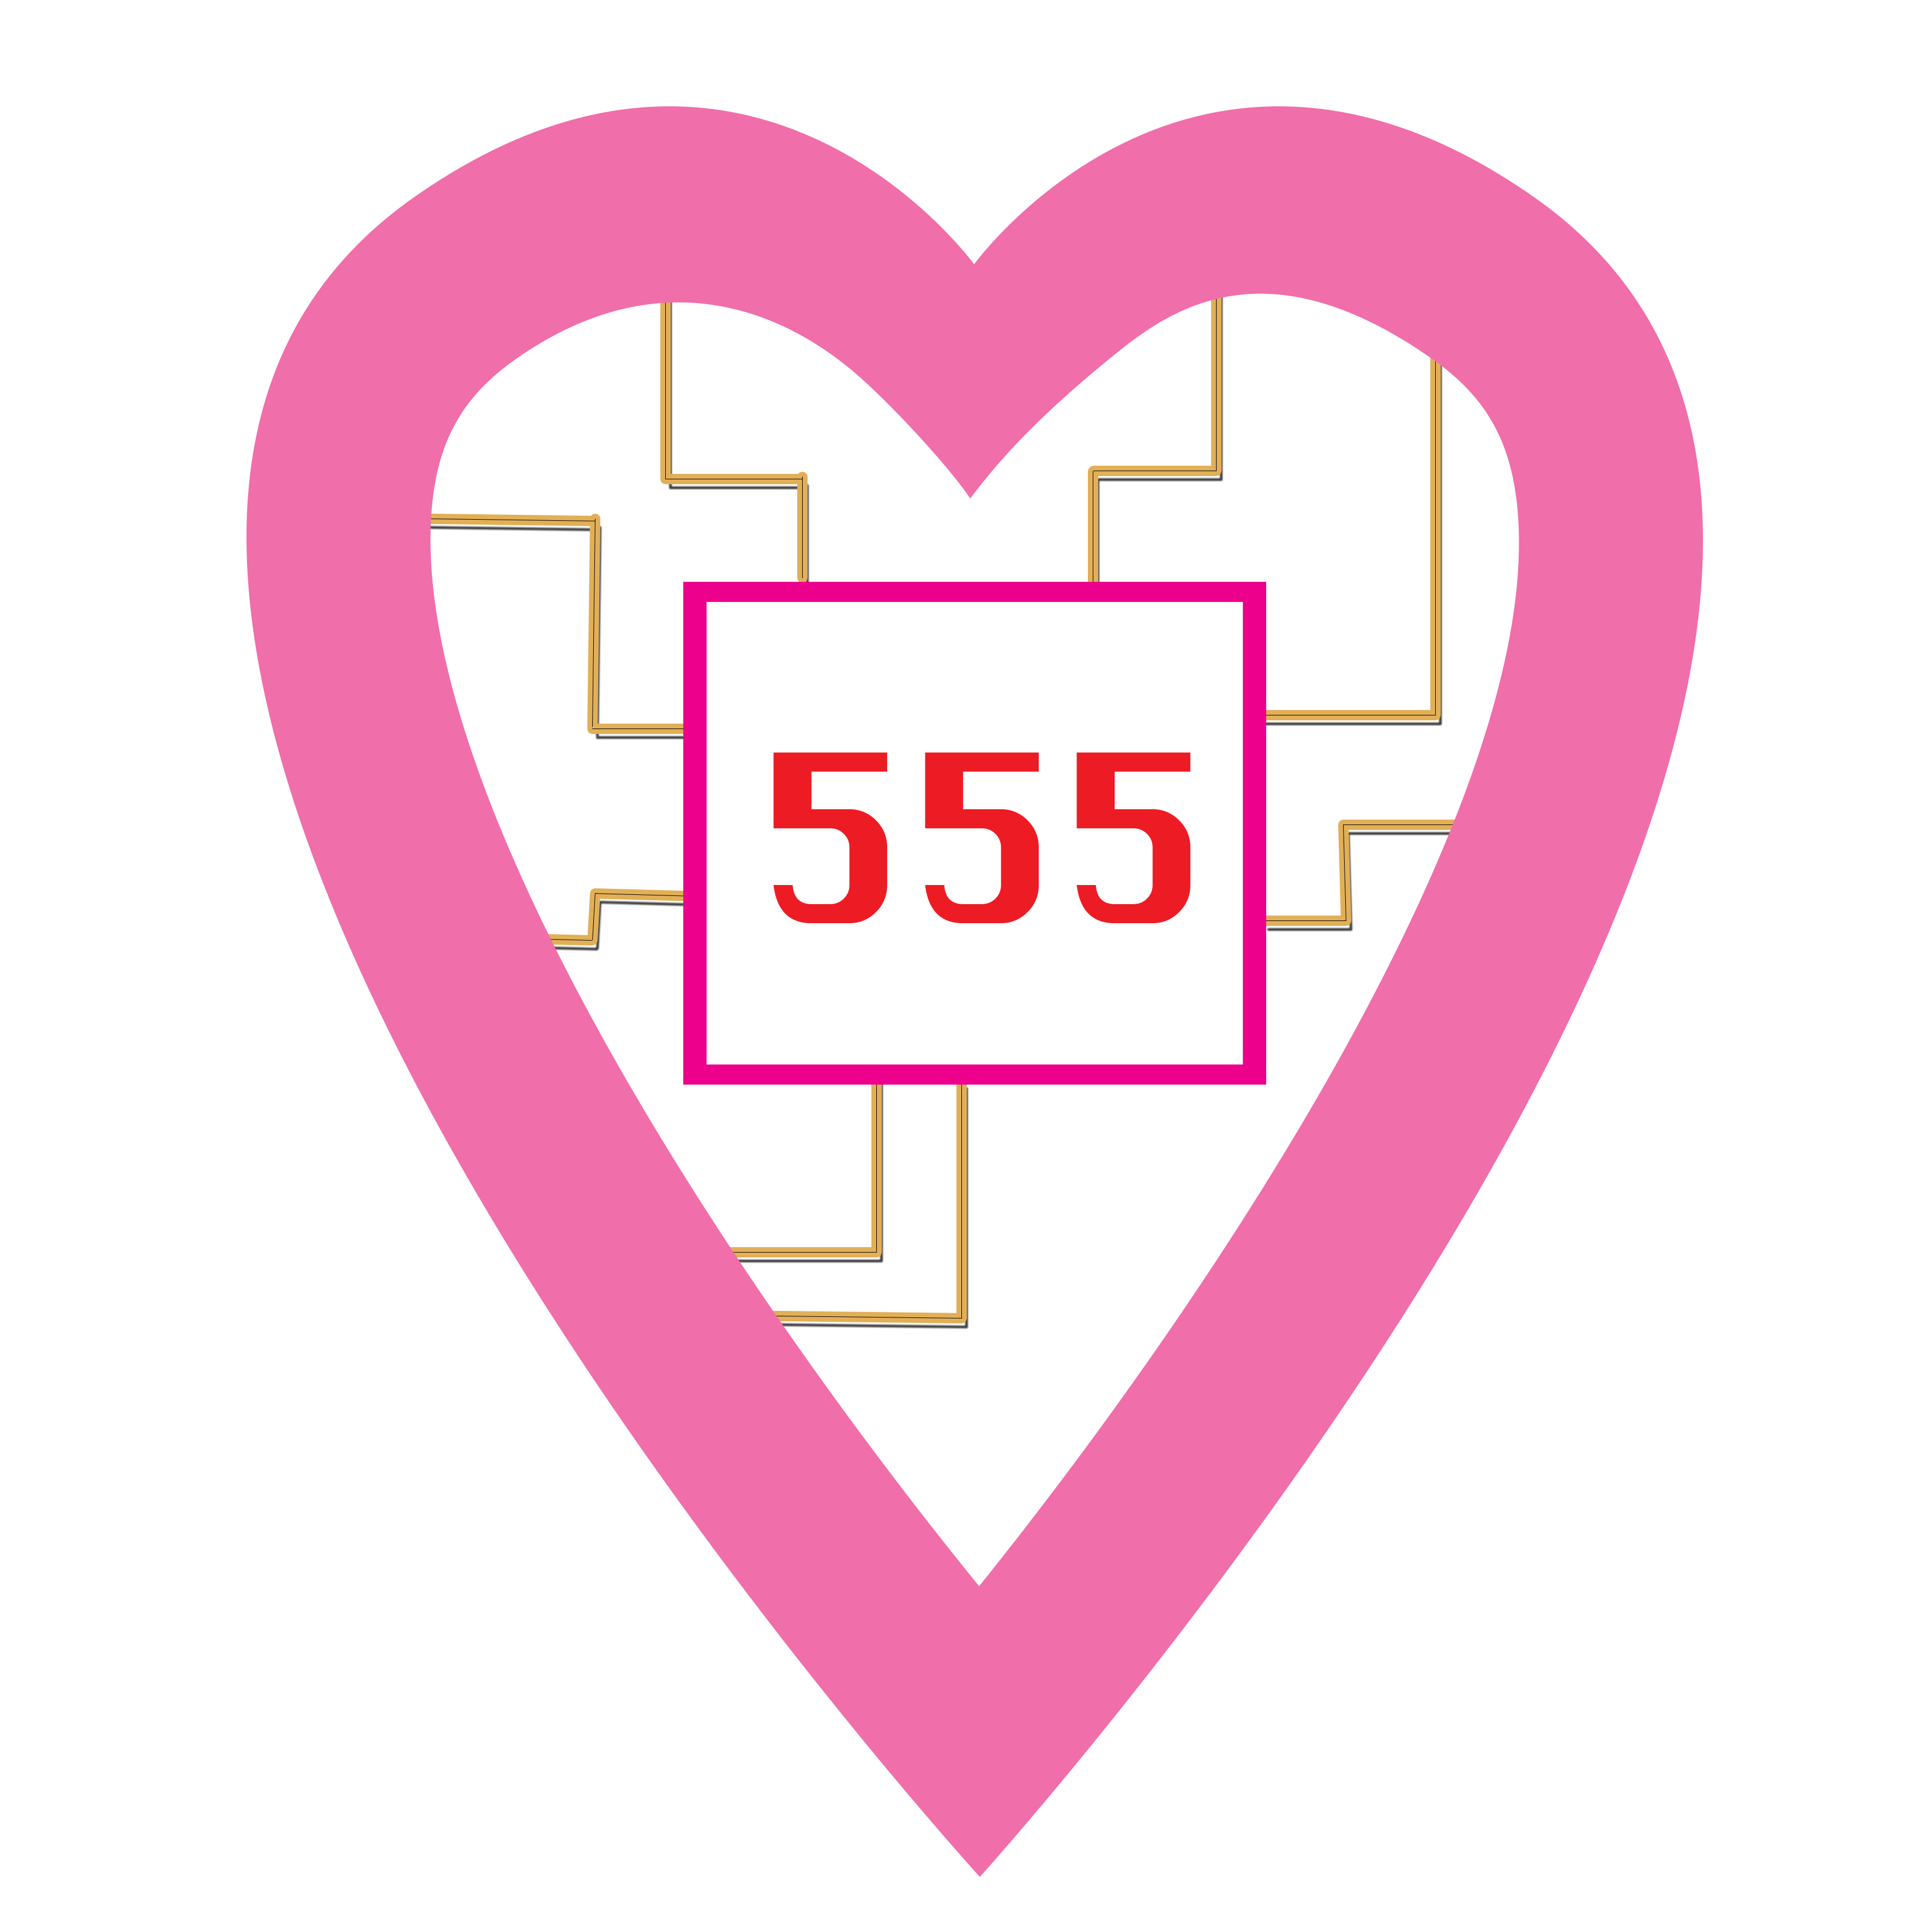
\includegraphics[height=10cm]{figures/titlepicheart.png}
 \end{center}
 \newpage 
\tableofcontents
\newpage

% Angry Birds In Real Life: Et legetøj


% Forside

% \begin{titlepage}
%     \centering
%     % \includegraphics[width=0.15\textwidth]{example-image-1x1}\par\vspace{1cm}
%     {\scshape\LARGE H. C. Ørsted Gymnasiet, Lyngby \par}
%     \vspace{1cm}
%     {\scshape\Large Forløb: Digitalt måleinstrument\par}
%     \vspace{1.5cm}
%     {\huge\bfseries \par}
%     \vspace{2cm}
%     {\Large\itshape Simon Rumle, Daniel Laporte og Christoffer Rasmussen\par}
%     \vfill
%     \par
%      \textsc{Klasse: TK 1, Fag: Teknik-Design og produktion}

%     \vfill

% % Bottom of the page
%     {\large \today\par}
% \end{titlepage}
\onehalfspacing %For at gøre indholdsfortegnelsen mere kompakt.
\section{Læsevejledning}
\todo{skriv om hvordan bilag og afsnit er nummereret og hvordan kilder er angivet}
\section{Projektbeskrivelse}
 
\subsection{Problemanalyse}
% Finder beviser for at angry birds ikke er godt for børn.
% 
% 
% 
I det moderne samfund bliver TV og iPads mere og mere inddraget i børns opvækst. Ifølge en undersøgelse af Northwestern University - Center of Human Development\footnote{Northern University; Parenting in the Age of Digital Technology - A national survey; revised 2014}, er 27\% af alle amerikanske familier
% side 8
 \emph{media-centric}, hvilket betyder at disse familier benytter en stor del af deres tid foran en digital skærm af en eller anden form, dette indebærer også deres børn. 

På trods af denne gængse tendens for IT-brug, udviser forældre en generel nervøsitet vedrørende konsekvenserne af børn (under 8 år) forbrug af digitale medier, herunder specielt computerspil. Ifølge undersøgelsen af Northwestern University, er forældre mest af alt nervøse om børns fysiske helbred og sociale evner som konsekvens af meget brug af computerspil på iPads og smart phones.
% side 6 
Selvom videnskaben om konsekvenserne af forbrug af computerspil stadig er ret tvivlsomt og på et tidligt forskningsstadie, er det en relevant problemstilling.

\subsection{Problemformulering}
\emph{Det er et samfundsmæssigt problem at børn har svære ved at socialiserer sig pga. de bruger for lang tid på smartphone apps.}


\subsection{Projektafgrænsning}
For at specificerer en løsning til denne problemstilling tages der udgangspunkt i videospillet Angry Birds af Rovio Entertainment. Ifølge Michael Chorost beskrevet i Psychology today\footnote{Chorost, Michael How I kicked my addiction to the iPhone game Angry Birds; \url{https://www.psychologytoday.com/blog/world-wide-mind/201101/how-i-kicked-my-addiction-the-iphone-game-angry-birds}; 2011}
er der 4 overordnede grunde til at Angry Birds er let at blive afhængig af:
\begin{itemize}
	\item Det er simpelt, ingen "learning curve".
	\item Det er en primitiv nydelse i at destruerer ting.
	\item Selve fysikken i spillet virker realistisk og forudsigeligt.
	\item Det er sjovt. Dyrene i spillet laver backflips og siger sjove lyde.
\end{itemize}

Vi har således tænkt os at udforme en fysisk udgave af et Angry Birds lignende spil, hvor børn kan interagerer socialt ved at spille mod hinanden i stedet for at sidde foran deres iPad. For at omgå copyright kalder vi vores produkt \emph{Moody Feathercreatures}.

Vi har opstillet et overordnet blokdiagram for hvordan vi har tænkt os at efterligne spillet. Se \Cref{fig:blok}.

Vi har valgt at lave et produkt der kan skyde nogle paptårne fra hinanden. Den skal også kunne justerer hastigheden på projektilet afhængigt af projektilets farve (ligesom farverne på fuglene i Angry Birds) og man skal kunne bruge en form for controller til at justere kanonens vinkel i forhold til vandret. Se \Cref{fig:skitse}.

\begin{figure}
	\centering
    \includegraphics[width=13cm]{figures/2_1projektbeskrivelse/blok.png}
	\caption{Blokdiagram af overordnet løsning. Input blokke(røde), Output blokke (gule), Kredse (grønne)}
	\label{fig:blok}
\end{figure}

\begin{figure}
	\centering
    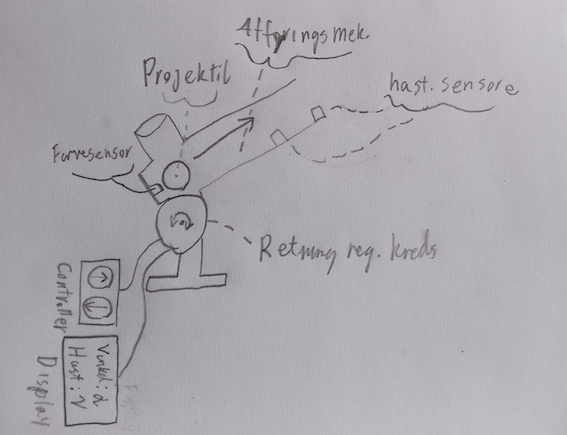
\includegraphics[width=13cm]{figures/2_1projektbeskrivelse/skitse.jpg}
	\caption{En overordnet skitse af produktet}
	\label{fig:skitse}
\end{figure}



Som man kan se på \Cref{fig:blok} er blokkende inddelt således:
\begin{itemize}
	\item Input blokke
	\begin{itemize}
		\item Ladningssensor
		\begin{itemize}
			\item Denne del skal kunne se på farven af et indsat projektil og derfra sende det til arduinoen.
		\end{itemize}
		\item Controller
		\begin{itemize}
			\item Til at bestemme retningen på selve "kanonen".
		\end{itemize}
		\item Hastighedsmåler
		\begin{itemize}
			\item For at kunne måle hastigheden ved udgangen af "kanonen".
		\end{itemize}
	\end{itemize}
	\item Output blokke
	\begin{itemize}
		\item Display
		\begin{itemize}
			\item Til at vise point og hastighed af projektilet. Muligvis andet.
		\end{itemize}
	\end{itemize}
	\item Kredse
	\begin{itemize}
		\item Hastighedsregulerende kreds
		\begin{itemize}
			\item Benyttes til at regulerer hastigheden af projektet afhængigt af dens farve.
		\end{itemize}
		\item Retningsregulerende kreds
		\begin{itemize}
			\item Benyttes til at bestemme retningen alt efter inputtet fra controlleren.
		\end{itemize}
	\end{itemize}
\end{itemize}



\subsection{Overordnede produktkrav}
Da vores produkt er beregnet til børn og unge, skal produktet være sikkert at bruge for børn og unge. Dette betyder at vores "kanon" ikke må skyde hårdt nok, til at volde skade på børn og unge. Derudover skal projektilet "kanonen" skyder, ikke være skarpt eller meget hårdt, da der er risiko for at børnene, ved en fejltagelse, skyder på hinanden. "Kanonen" og projektilet skal være i stand til at vælte papboksene ned. Vi skal sikre os as vores "kanon" og projektil ikke er i strid med den danske våbenlov, og eventuelt udenlandske våbenlove.
Vores produkt skal altså opfylde følgende overordnede produktrav:
\begin{itemize}
\item Sikkert at bruge for børn.
\item Projektilerne skal ikke have en farlig form.
\item Produktet skal skyde hårdt nok til at vælte små papbokse.
\item Produktet skal ikke være i strid med våbenloven.
\end{itemize}



\subsection{Tidsplan for projektet}
\begin{figure}[H]
	\centering
    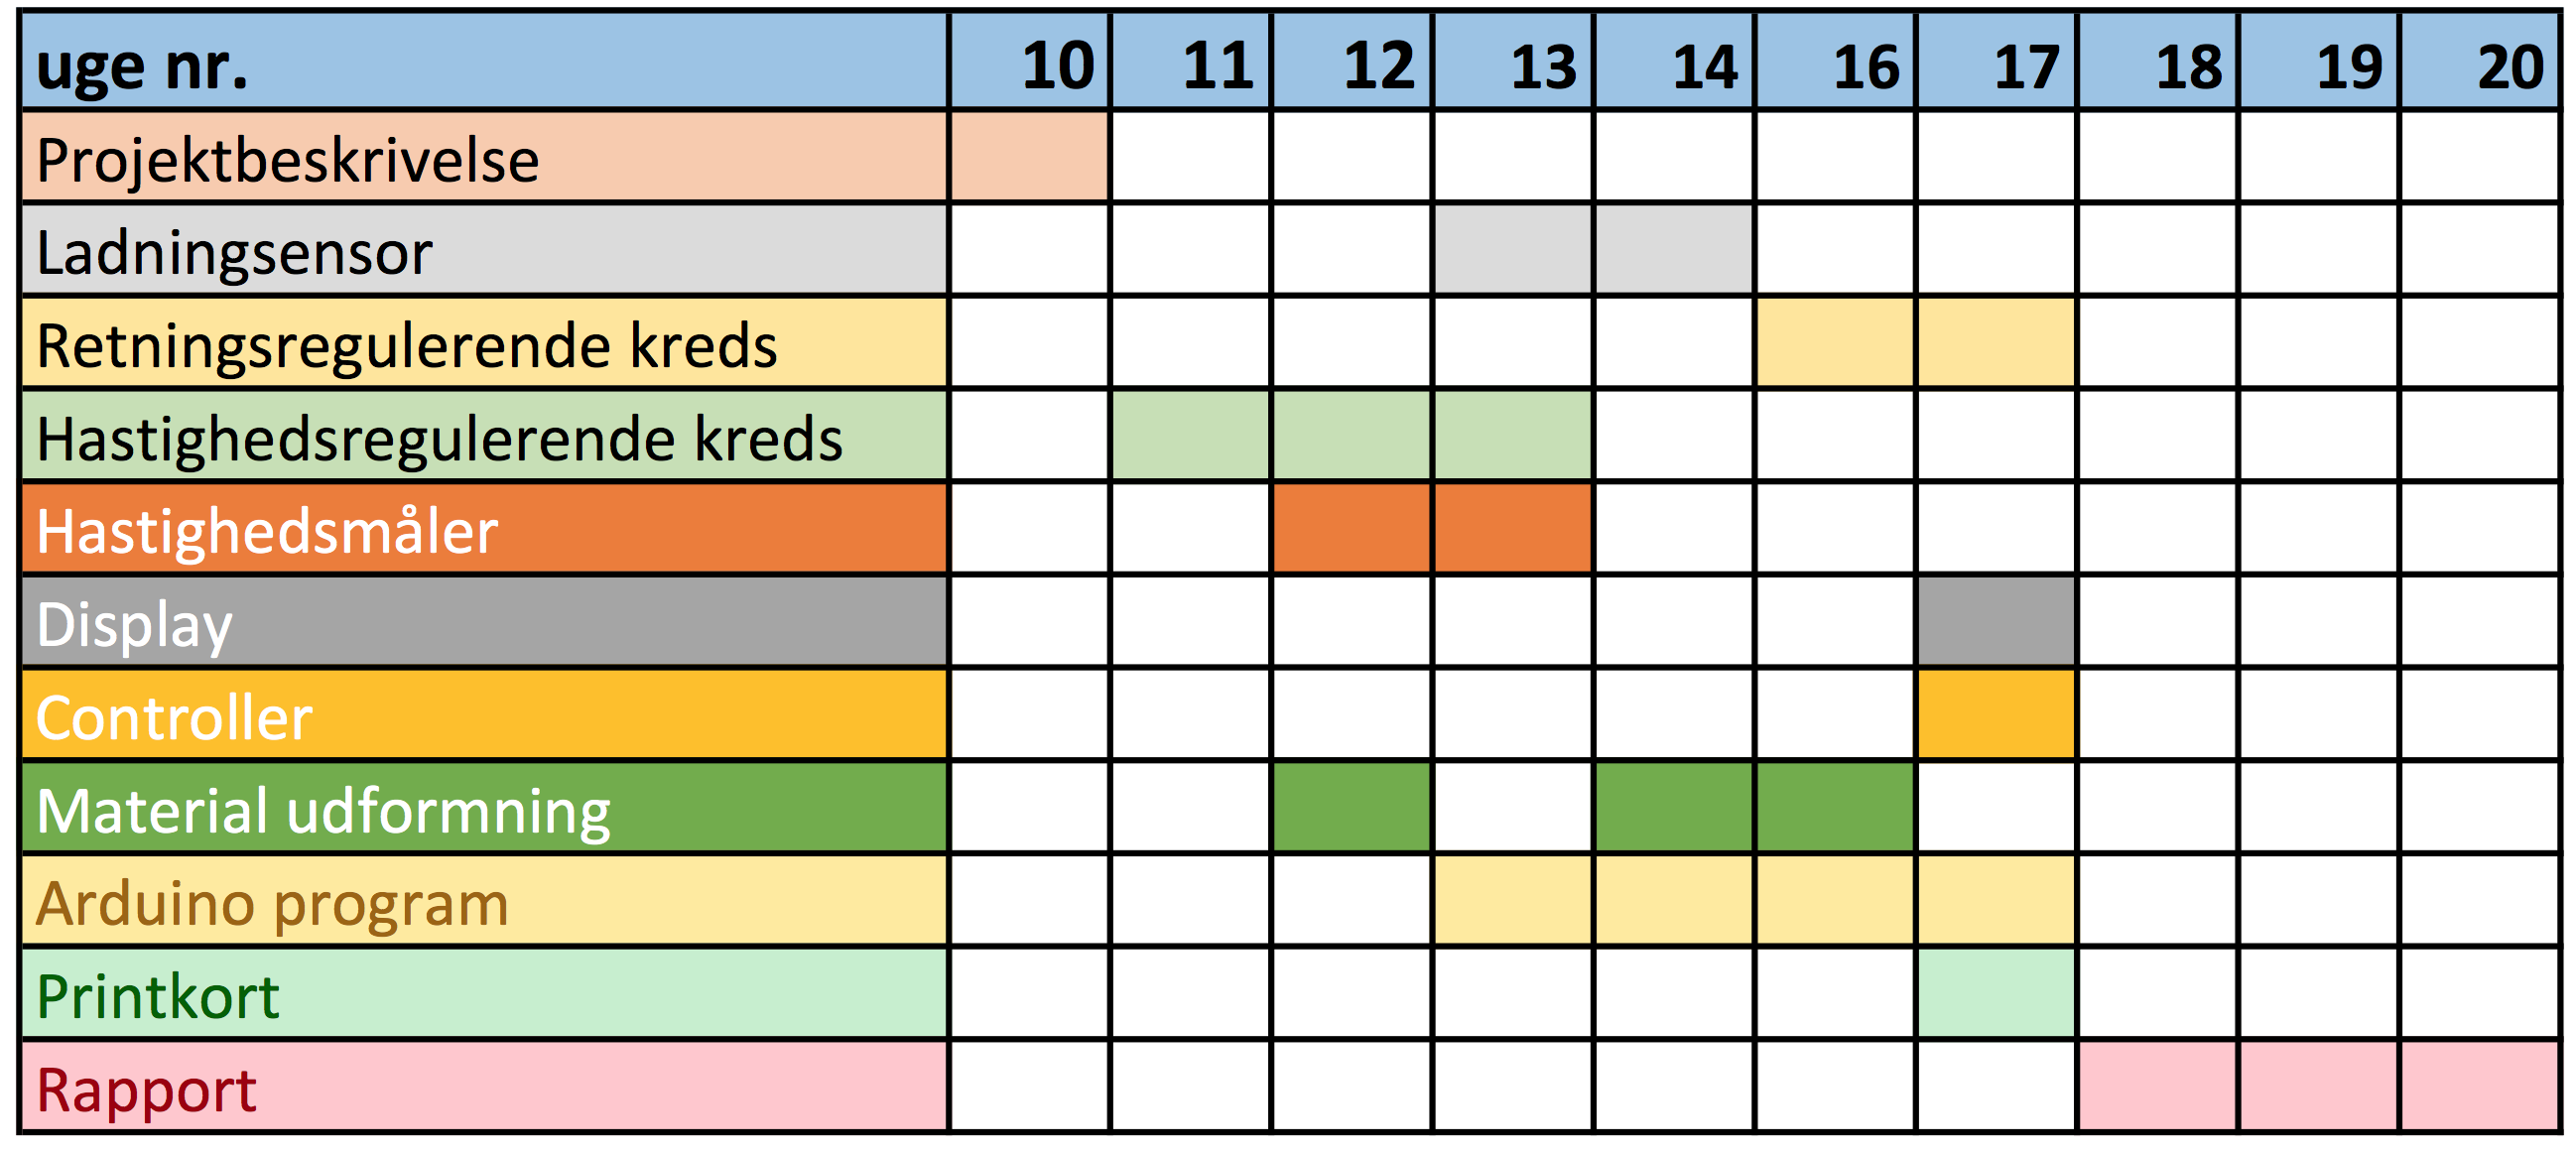
\includegraphics[width=15cm]{figures/2_1projektbeskrivelse/tidsplan.png}
	\caption{Tidsplan}
	\label{fig:tidsplan}
\end{figure}



\input{files/chapters/2_2kravspecifakation}
\section{Overordnet løsningsforslag}

Vi har gennem vores idegenerering kommet frem til to overordnet løsningsforslag. Vi kom frem til at den mest kompliceret dele af kredsen som er vigtigst at designe, og have på plads fra begyndelsen er affyringsmekanismen.
% Mesk kompliceret? Bedre formulering
Heraf har vi kommet frem til to typer afføringsmekanismer: \emph{Gauss-kanon} og \emph{Elastik-kanon}.
Som overordnet løsning til hastighedssensoren har vi tænkt os at se på om vi kan udforme et pass band filter og IR lyd til at sanse hvornår bolden kommer forbi.

\subsection{Gauss-kanon}
Her har vi tænkt os at benytte princippet om magnetfelter i spoler til at drive et projektil fremad. Heraf kan vi ved at variere i den tilførte strømstyrke og spænding for at ændre magnetfeltet.
Ud fra vores brainstorm har vi to måder at udforme sådan en affyringsmekanisme: Magnetisk løb og Magnetisk aftrækker
\subsubsection{Magnetisk løb}
\begin{figure}[H]
	\centering
    \frame{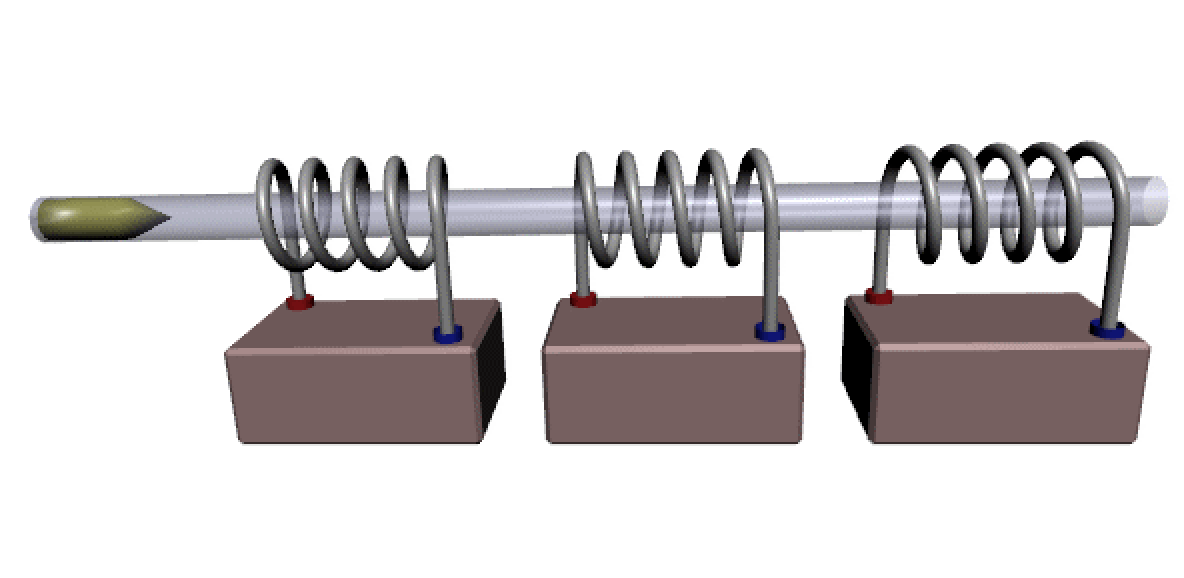
\includegraphics[width=10cm]{figures/2_3overordnetvalg/loeb.png}}
	\caption{Et billede af en gausskanon, hvor projektilet bliver accelereret af tre spoler. Kilde: \cite{WikiGaussCanon}}
	\label{fig:loeb}
\end{figure}
For en enkelt spole, kan et projektils udgangshastighed modelleres udtrykket udformet af PhD i anvendt matematik Don Pettibone (se \cite{gaussRifleModel}).
% Model
\[
	v_{slut} = \frac{\mu_0 \cdot N_0 \cdot I_0}{2 \cdot r_0} \cdot \sqrt{\frac{2 \cdot \mu_r - 1}{\rho \cdot \mu_0}}
\]
\begin{itemize}
	\item $v_{slut}$: Sluthastigheden ved enden af spolen for projektilet $[\frac{\si{m}}{\si{s}}]$
	\item $\mu_0$ : Vakuumpermeabiliteten ($\mu_0 = \SI{1.257d-6}{\frac{T \cdot m}{A}}$).
	\item $I_0$ : Strømstyrke $[A]$.
	\item  $\mu_r$: Relativ permeabilitet af projektilets materiale.
	\item $r_0$: Radius af spolen $\si{[m]}$.
	\item $N_0$: Antallet af vendinger for spolen.
\end{itemize}

Dog er modellen meget optimistisk og i et reelt eksempel (se \cite{HighEffectExample}) udført af elektro-inginøren Mehdi Sadaghdar så vurderer vi at vi kan let komme til at arbejde med effekter på omtrent:
\[
	P \approx \SI{2000}{W}
\]
Måder vi kan holde os fra så store effekter er at benytte jernkerne, for at øge den relative permeabilitet og magneter. Dette er svært at implementere i en Magnetisk løb løsning, idet spoler med jernkerne sjældent har et hul et projektil kan passere. Det er dog lettere at få implementeret i Magnetisk aftrækker løsningen.

En anden måde at få implementeret Magnetisk løb løsningen ved brug af lavere effekter er at benytte et par (knap så lange) solenoider, for at danne en længere spole, således benytte en kombination af sensorer og transistorer til at slukke for den tidligere spole og tænde den næste for at sikre sig at den bliver ved med at accelerer undervejs.

\subsubsection{Magnetisk aftrækker}
Den Magnetiske aftrækker fungerer ved at placerer en magnet tæt ved en slukket spole. Hvis magneten berøre spolens ende der har en tilsvarende ladning vil de afstøde hinanden og således affyre projektet. Se \Cref{fig:MagShooter}.
\begin{figure}[H]
	\centering
    \frame{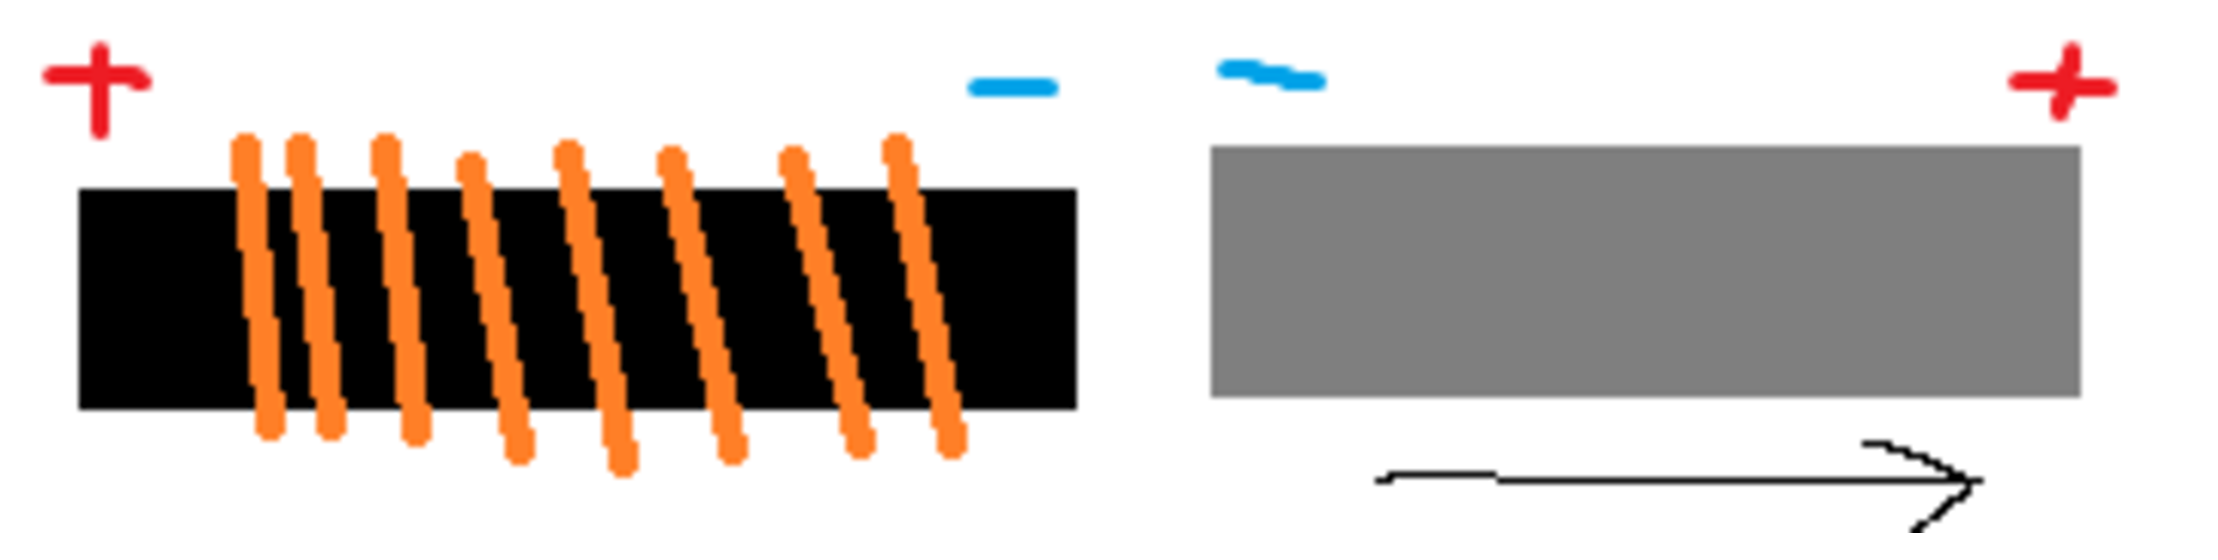
\includegraphics[width=10cm]{figures/2_3overordnetvalg/MagShooter.png}}
	\caption{Et billede af en spole på venstre side, der benyttes til at affyre et magnetisk projektil på højre side.}
	\label{fig:MagShooter}
\end{figure}

Denne løsning er dog svære at matematisk modellere, men med sikkerhed må det gælde at (se \cite{Orbit2009} - side 129), hvis der benyttes jernkerne
\[
	B = \mu_r \cdot \mu_0 \cdot \frac{N_0 \cdot I_0}{l}
\] 
Hvor $B$ er magnetfeltstyrken $[\si{T}]$ og $l$ er længden af spolen $[\si{m}]$. Her fremgår det at hvis $\mu_r$ bliver meget høj (hvilket den kan blive med jernkerne), vil magnetfeltet stige proportionalt. Med passende legeringer kan man få en relativ permeabilitet på op til \num{15000}.


Ulempen ved denne løsning er dog at der nok skal være ret så høj en effekt der skal sendes gennem spolen indenfor et kort tidsrum for at få det til at virke.

\subsection{Elastik-kanon}
Denne løsning bliver vores produkt udformet som en slangebøsse med variabel styrke. Således bliver den variable: hvor langt væk elastikken trækkes væk fra hviletilstand.
En model for dette princip kan simpel konstrueres ud fra energiomdannelse fra potentiel energi i Hooks lov til kinetisk energi.
\begin{align}
-k \cdot x &=\frac{1}{2} \cdot m \cdot v^2 \\
 \iff v	&= \sqrt{\frac{-2 \cdot k \cdot x}{m}} 
\end{align}
\begin{itemize}
	\item $k$: Fjederkonstanten for benyttet elastik $\si{[\frac{N}{m}]}$
	\item $m$: Massen af projektilet $\si{[kg]}$
	\item $v$: Udgangshastigheden af projektilet $\si{[\frac{m}{s}]}$
	\item $x$: Afstand fra hviletilstand $\si{[m]}$
\end{itemize}

Vores implementering af en elastik-baseret løsning er at vi benytter os af en snor der er forbundet til elastikken og et hjul, hvor hjulet drejes af en motor (se \Cref{fig:elasticshooter}). For at sikre os at projektilet bliver affyret benytter vi gear, så når optrækning-mekanisme trækker snoren er hjulet i gear, hvorimod når vi skal affyre projektilet sættes den i frigear. Dette kan gøres ved at lade en motor være den der trækker snoren op, og en anden motor være den der ændrer gear.
\begin{figure}[H] 
	\centering
    \frame{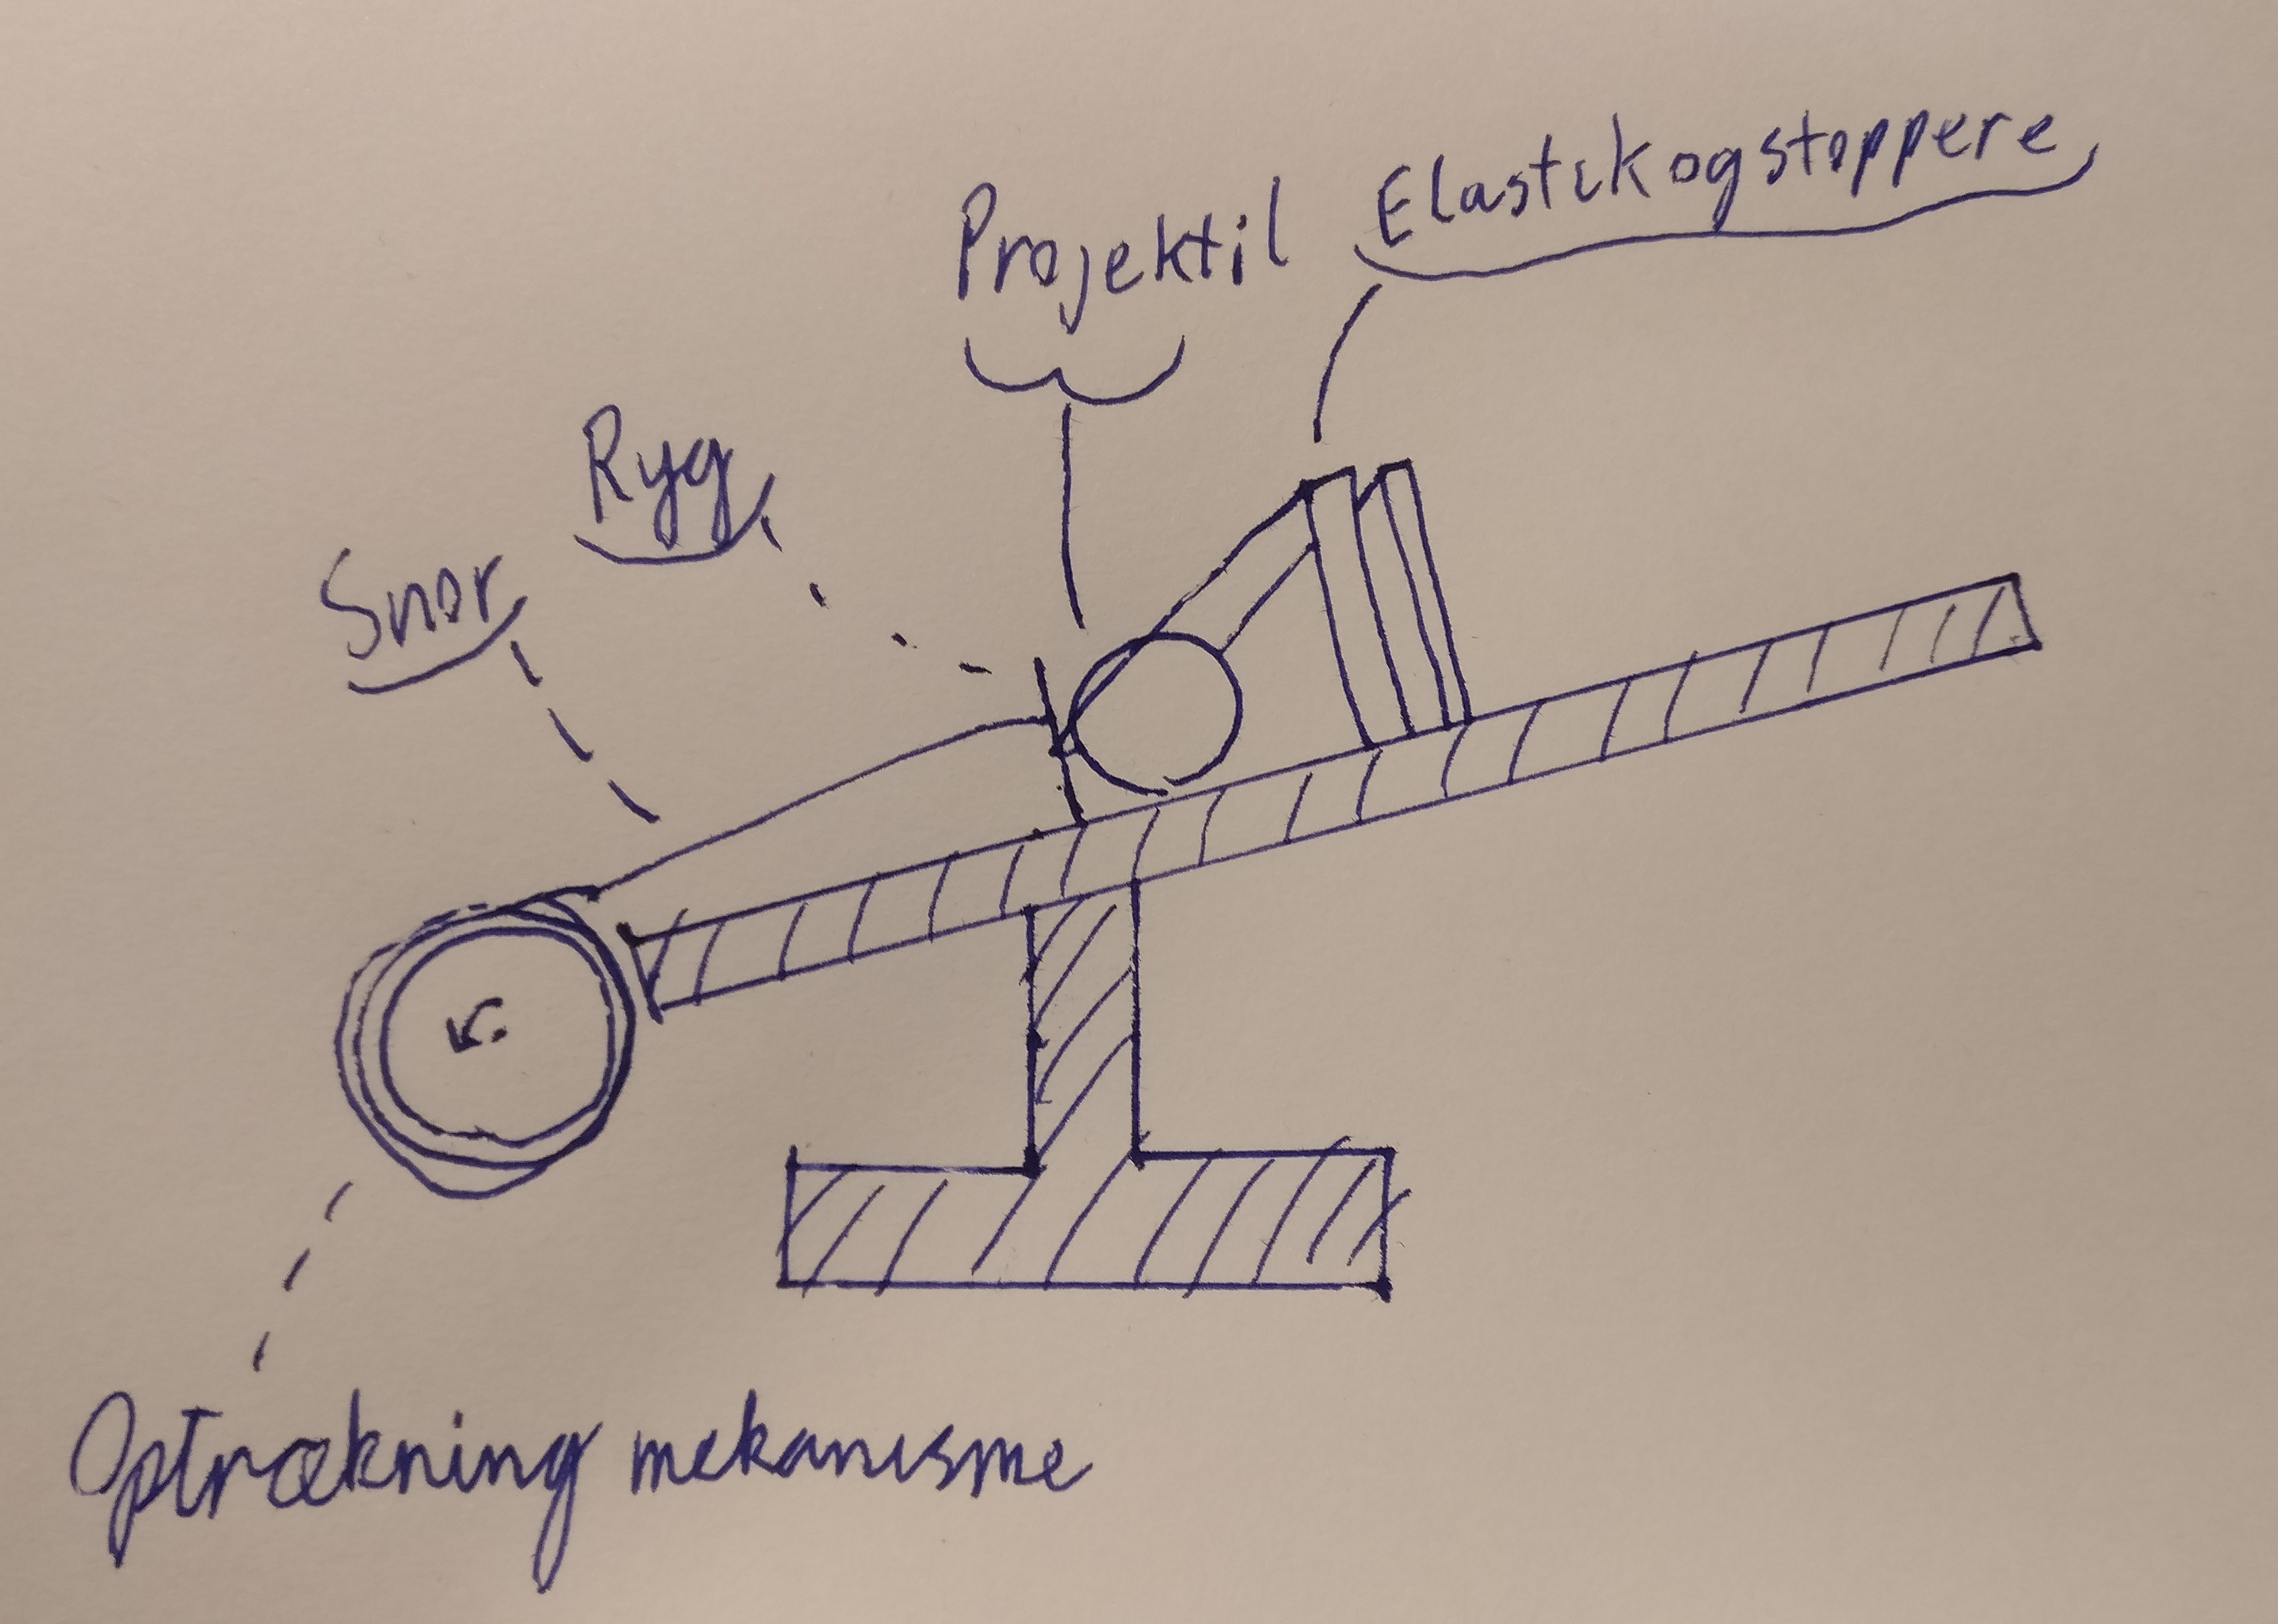
\includegraphics[width=13cm]{figures/2_3overordnetvalg/ElasticShooter.jpg}}
	\caption{Affyringsmekanisme for en Elastik-kanon, der er ikke fokus på andre blokke beskrevet i projektbeskrivelse.}
	\label{fig:elasticshooter}
\end{figure}


\subsection{Valg af overordnet løsning}
Vi har valgt at udarbejde en Elastik-kanon, idet vi synes hvor får en del EL-problemer at se til i forhold til hastighedssensoren. Samt hvis vi skulle udarbejde en Gauss-kanon, ville vi bruge lang tid på at teste for vakuumpermeabilitet og benytte høje strømstyrker, hvilket i sig selv kunne give en del problemer, da vi ikke ved meget om at arbejde med høje strømstyrker. Samt ville man kunne argumentere for at så høje strømstyrker som benyttes i forbindelse med en Gauss-kanon kan muligvis være for farligt til et børnelejetøj.



%%%%%%%BLOKKE MEGET VIGTIGT%%%%%%%%
\section{Samlet kredsløb}
Vores kredsløb er delt op i mange forskellige delkredsløb som er med til at styre vores kanon. Her har vi 3 motorer til at styre fysiske bevælgelser. Hertil har vi en farve sensor og infrarøde sensorer til at læse projetilets hastighed og farve. Her bruges arduinoen til at kordinere disse delkomponenter.

\todo{insæt billede af det fulde kredsløb}

\subsection{hastighedsmåler}
Her er der brugt en 555-timer til at lave en puls, som sendes til modtager delen som så forstærker signalet og og der bliver brugt en peak detector far at få et stabilt signal der så kan sendes til arduinoen.
 \subsection{farve sensor}
Denne del fungere ved at der er 3 lysdioder. en rød, en grøn og en blå. ardinoen giver et signal om hvilken diode der skal være tændt hvorved at en phototransistor opfanger det lys der bliver reflekteret dette give så forskællige værdier i forhold til hvilken farve der reflekterende objekt har. dette signal bliver sendt tilbage til arduinoens analog input.
\subsection{controller}
Inputet er bare et par knapper som går direkte ind i arduinoens digitale porte.
På samme måde bliver displayet også for det meste tilkoplet direkte til arduinoen odover en enkelt 10k potentiometer som bruges.
\subsection{moterkontrol}

Vi har to forskellige motere til at styre vores kanon. en til at dreje den op og ned og 2 til at styre dens skyde mekanisme. Den ene bliver brugt til at hive i elestikken mens den anden er en trigger som holder tandhjulene sammen som giver mulighed for at motoren elastikken bevæger sig frit for motoren.

\section{Retningsregulerende kreds}
\begin{figure}[H]	
	\centering
    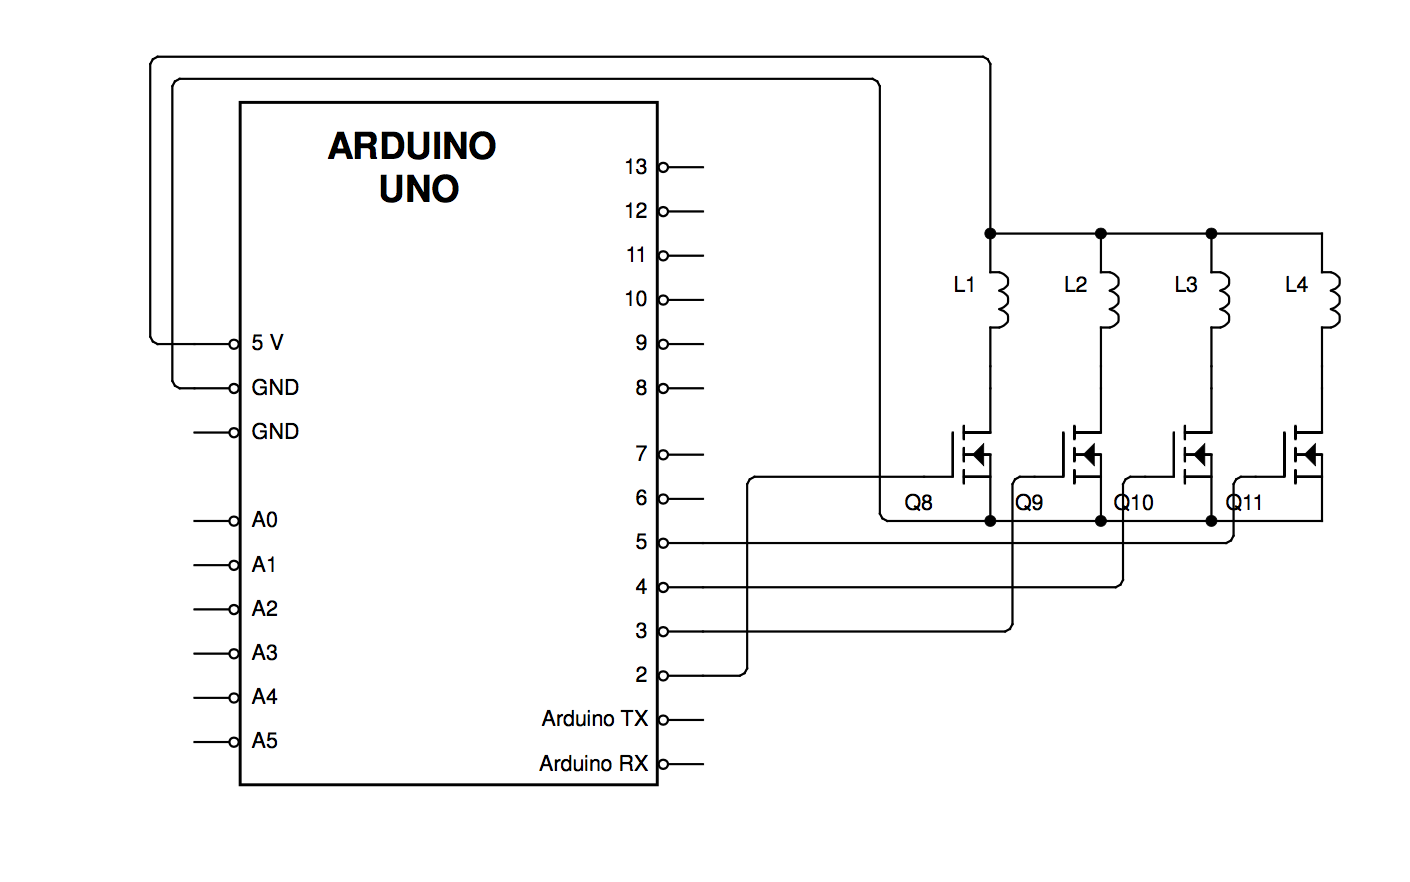
\includegraphics[width=13cm]{figures/CIRCUITS/steppermotorFinal.png}
	\caption{Et billede af kredsløbet for den retningsregulerende kreds.}
	\label{kreds:retning}
\end{figure}
I vores retningsregulerende kreds, har vi valgt at benytte en stepper motor, til at styre hvilken vinkel bolden skydes ud i. Her der bliver der brugt en ekstern strømforsyning på $\SI{5}{V}$, så der kan løbe nok strøm igennem spolerne i stepper motoren. For at bruge den eksterne strømforsyning bruger vi MOSFETs som digitale switches.
\todo{lav kredsen om igen, således at dioden over mosfettet er med, se MOSFET}
\subsection{Komponenter}
\subsubsection{N-Channel power MOSFET - F12N10L}
\begin{figure}[H]
	\centering
    \frame{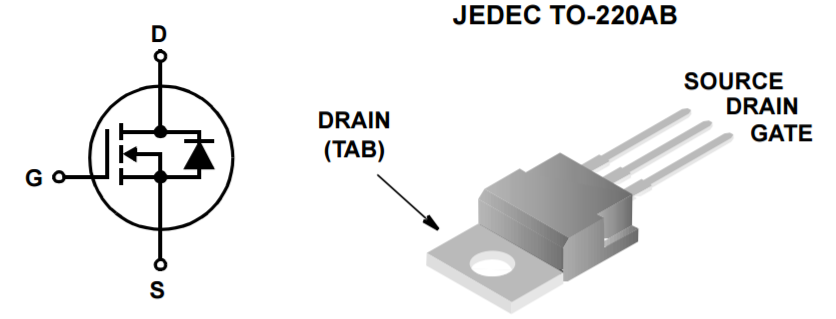
\includegraphics[width=10cm]{figures/komponenter/F12N10L.png}}
	\caption{Pindiagram og symbol af F12N10L. Kilde:\cite{kompMOSFET}}
	\label{fig:kompMOSFET}
\end{figure}
På \Cref{fig:kompMOSFET} er der et symbol og pindiagram over MOSFET komponenten.
Denne MOSFET er bygget til $\SI{5}{V}$ logik, samt har det en lav rise og fall time på et par hundrede nanosekunder og således vil det fungerer fint for en steppermotor. Databladet vi har benyttet kan findes i kilde \cite{kompMOSFET}. 
\todo{skriv om spændingsreguleret - derfor er det godt med arduino}

\subsubsection{Stepper motor - RS191-8328}
\begin{figure}[H]
	\centering
    \frame{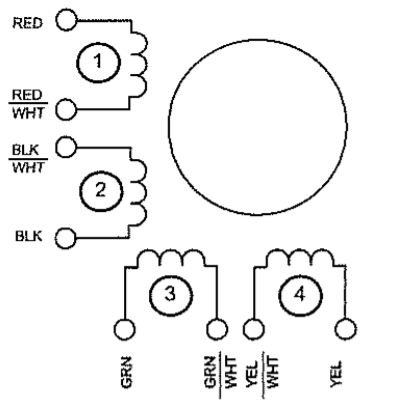
\includegraphics[width=10cm]{figures/komponenter/RS191-8328.png}}
	\caption{Diagram af RS191-8328. Kilde: \cite{kompstepmotor}}
	    \label{fig:kompstepper}
\end{figure}

\todo{Har brug for noget tekst under billedet}

\subsubsection{Arduino}
Se afsnit \ref{sec:arduino}.

\subsection{Teori}
\subsubsection{MOSFET}
Vi benyttede MOSFET for at få en højere strøm igennem spolerne end Arduinoen kan levere. Med en MOSFET kan man kontrollere hvor meget strøm der løber gennem Gate til Source, med spændingsfaldet over Drain og Source. Dette gør en MOSFET optimal som en digital switch. 
\subsubsection{Stepper motor}
Vi benyttede en stepper motor til at styre hvor meget vi drejer kanonen. En stepper motor fungere ved at vi har et vis antal "steps" på en omdrejning. Man kan sende strøm gennem en af spolerne, som så vil trække stepper motoren et "step" frem eller tilbage. Man sender så skiftevis strøm igennem spolerne, for at få stepper motoren til at forsætte i en retning. Vores stepper motor har 200 "steps" på en omdrejning. 
% HVILKET -POLAR ER DET??
\todo{Husk at angive Uni-polar eller Bipolar ***}
%\subsection{Beregninger}

\subsection{Test}
Vi benyttede et Stepper library fra firmaet Arduinos hjemmeside\cite{steppercode:stepbystep}. Koden kan ses på Figur ~\ref{fig:steptest}. \todo{References fungerer meget underligt. Burde sige Figur 10}

% ---------------------BEGIN CODE
\begin{figure}[H] 
\caption{Kode til steppermoter for at angive antal steps der skal roteres}
\label{fig:steptest}
\begin{lstlisting}
#include <Stepper.h>
// Antallet af steps på vores motor
const int stepsPerRevolution = 200;  

// Initialiserer stepper biblioteket i pin 2 til 5:
Stepper myStepper(stepsPerRevolution, 2, 3, 4, 5);

// Antallet af steps motoren har taget
int stepCount = 0;         

void setup() {
//Initialiserer serial porten
  Serial.begin(9600);
}

void loop() {
  // Step et step:
  myStepper.step(1);
  Serial.print("steps:");
  Serial.println(stepCount);
  stepCount++;
  delay(500);
}
\end{lstlisting}
\end{figure}
% -------------------END CODE

Det fungerede fint efter hensigten og vi kunne let styre antallet af steps

% Hastighed 50
\section{Hastighedsregulerende kreds}
\begin{figure}[H]	\label{kreds:hastighed}
	\centering
    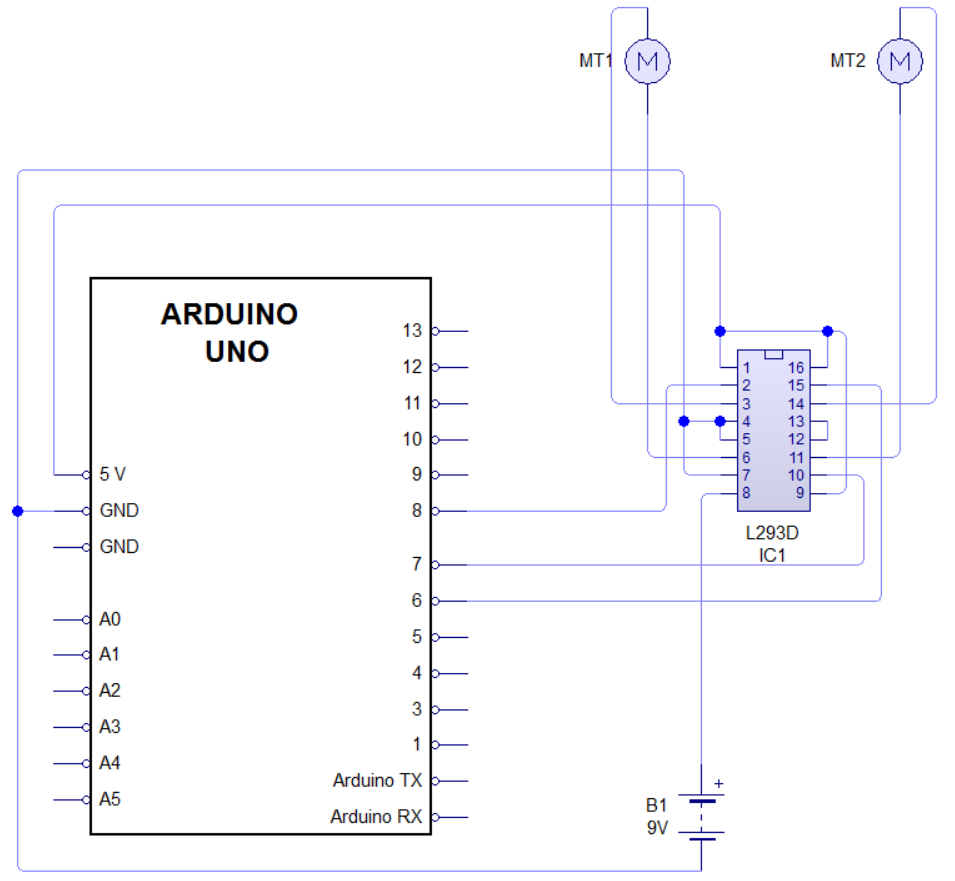
\includegraphics[width=10cm]{figures/2_4kredse/hastighed.png}
	\caption{Et billede af kredsløbet for den hastighedsregulerende kreds.}
\end{figure}
Som der kan ses på Figur \ref{kreds:hastighed}, er der motorene MT1 og MT2. Heraf gælder det at MT2 fungerer som et gear og MT1 fungerer som selve elastik-optrækkeren. Når motoren trækkes op løber der først strøm fra Arduinoens pin 6 
 %*** eller pin 6?
 hvorfra gennem L293D pin 14 kan strøm løbe gennem MT2 og låse gearet fast. Derefter sendes der strøm gennem Arduinoens pin 8 som trækker MT1 op. 
Til sidst slukkes for signalet til MT1 og derefter ændres polariteten i MT2, så affyringsmekanismen er i ``frigear''. Det skal således bemærkes at MT2 modtager 2 signaler fra arduinoen for at kunne vende polariteten.

\subsection{Komponenter}
\subsection{Lego $\SI{9}{V}$ DC motor}
Vi kunne ikke finde et specifik datablad, men vi ved at normal lego-mindstorm DC motor der kører på $\SI{9}{V}$, hvilket er fint til vores formål. 
\subsection{Dual H-bridge motor driver - L293D}
\begin{figure}[H] \label{fig:pindiagramL293D}
	\centering 
    \frame{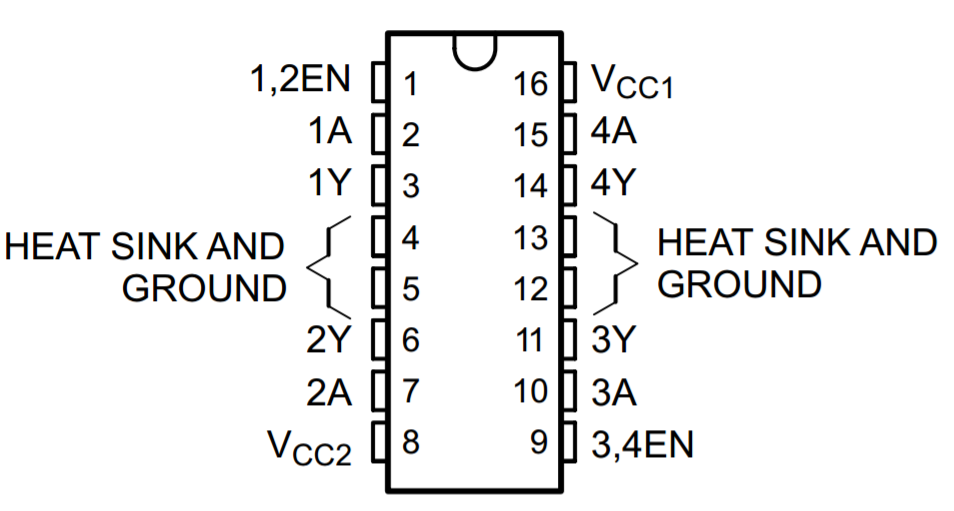
\includegraphics[width=10cm]{figures/komponenter/L293D.png}}
	\caption{Pindiagram af L293D}
\end{figure}
Pindiagram kan ses på Figur \ref{fig:pindiagramL293D}. Pin 1 og 9 er aktiverings pins for H broerne. Pin 1 aktiverer H broen på venstre side og pin 9 aktiverer H broen på højre side. Pin 2 og 7 bruges til at styre motoren koblet til 3 og 6. Pin 10 og 15 styre motoren på 11 og 14. Pin 4,5,13 og 12 er forbundet, og skal forbindes til jord. Kilde for komponentet: \cite{komphbridge}.
\subsection{Teori}
% \subsubsection{DC motor} *** Måske skriv
\subsubsection{H bridge}
En H-bridge er et komponent der benyttes til at vende polariteten i vores DC-motor som fungerer som gear. Dette gøres overordnet ved at H-formede kredse med switches der kan enten være on eller off. 
\begin{figure}[H]
	\centering
    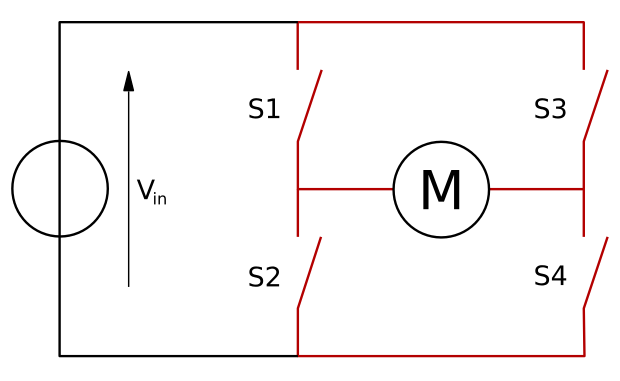
\includegraphics[width=13cm]{figures/2_4_3hastighed/hbridge.png}
	\caption{Et billede af en H-bridge, selve H-bridge struturet er markeret med rød. Kilde: \cite{teorihbridge}}
	\label{fig:hbridge}
\end{figure}
Det fremgår på Figur \ref{fig:hbridge} at switchene 1 til 4 er åbne. Disse switches kan så hvis de modtager et signal kan man forbindes således at strømmens retning løber i en bestemt retning. F.eks. Hvis S1 og S4 er lukkede switches, vil motoren løbe i en retning, end hvis S3 og S2 er lukkede switches. Kilde: \cite{teorihbridge}. 

%\subsection{Beregninger}

\subsection{Test}
\todo{Vi skal not beskrive hvordan vi testede denne kreds og have noget kode på det. ***}
\section{Hastighedsmåler}
\todo{Vi skal have skrevet til IR modtager og IR afsender}
\begin{figure}[H]
	\centering
    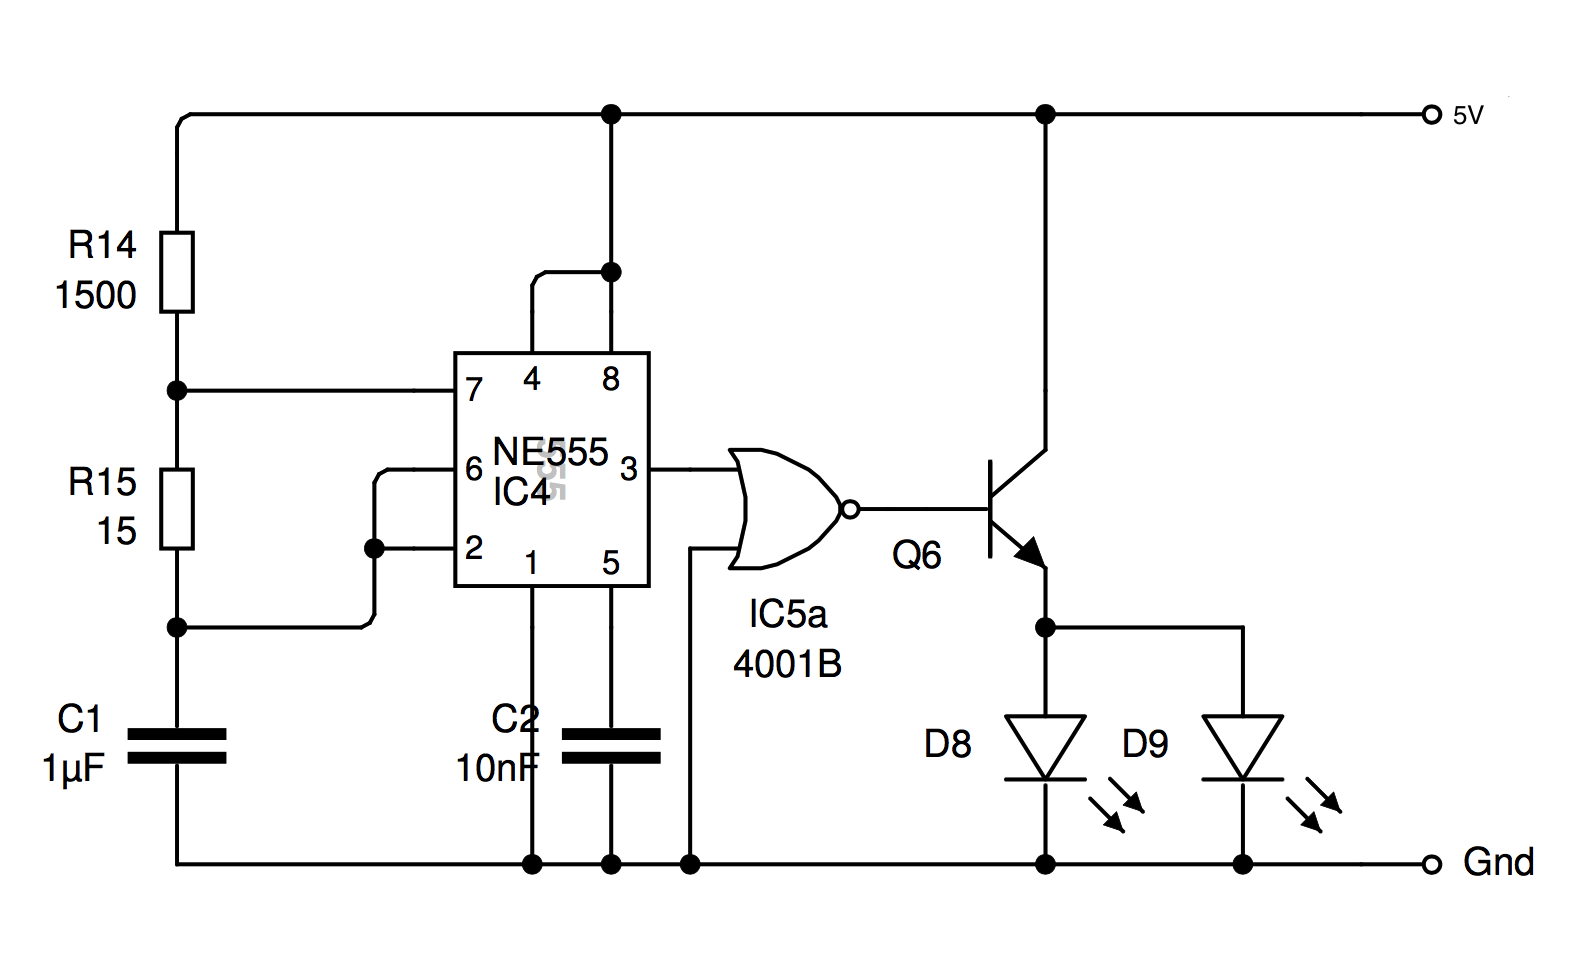
\includegraphics[width=13cm]{figures/CIRCUITS/IRafsenderFinal.png}
	\caption{IR-afsender}
	\label{fig:IRafsender}
\end{figure}
\begin{figure}[H]
	\centering
    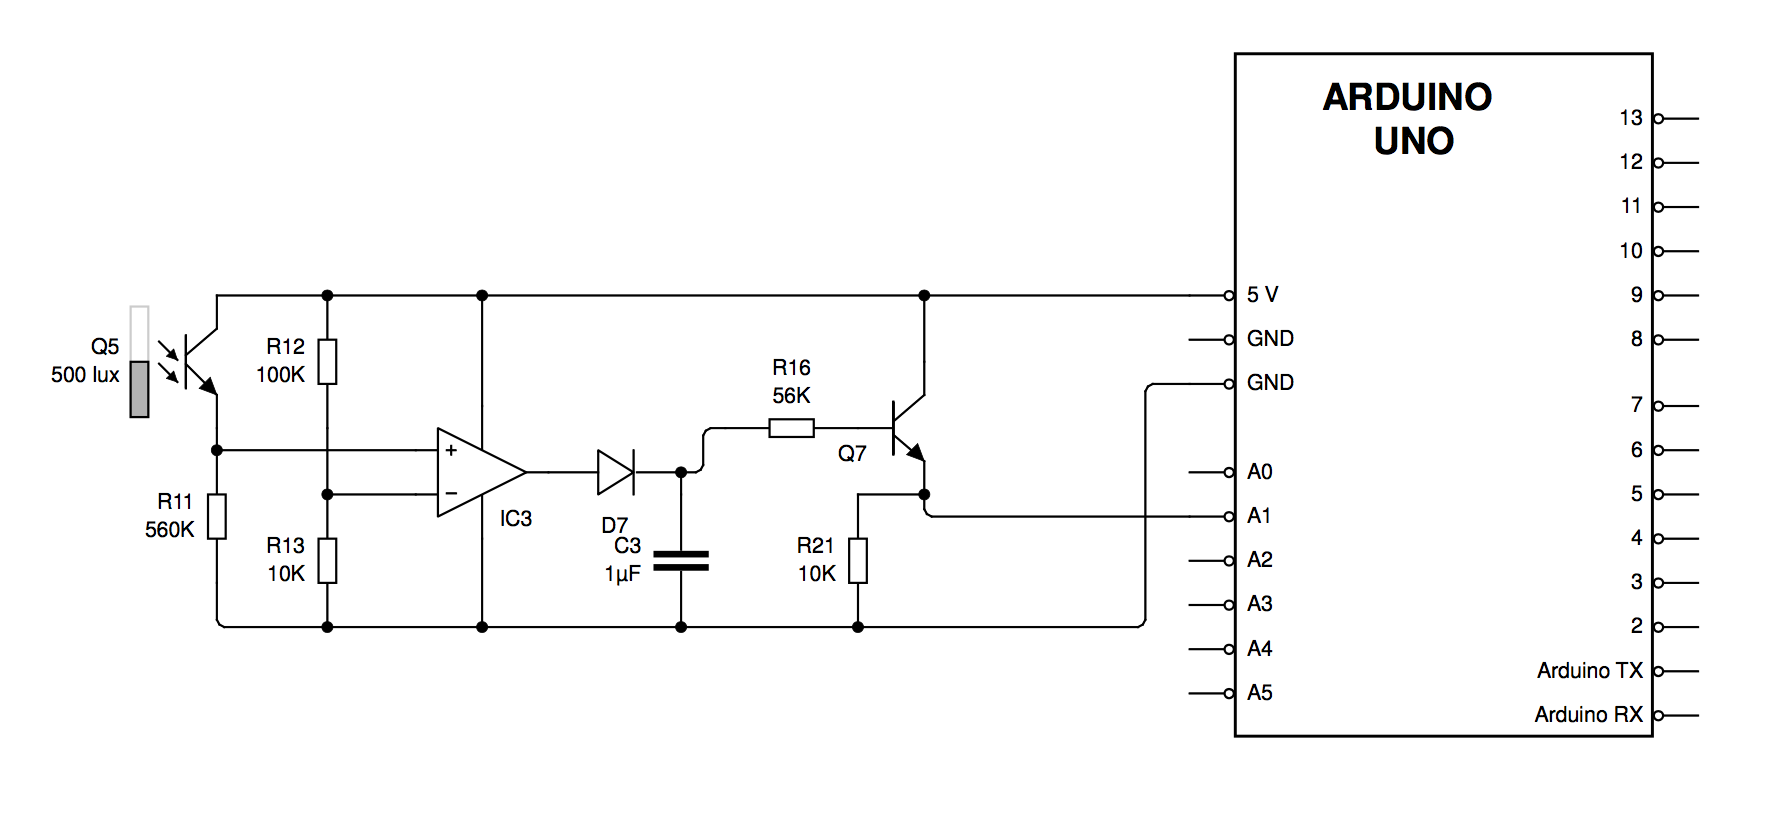
\includegraphics[width=17cm]{figures/CIRCUITS/IRmodtagerFinal.png}
	\caption{IR-modtager}
	\label{fig:IRmodtager}
\end{figure}



På Figur \ref{fig:IRafsender} modtager en 555 timer strøm fra en \SI{5}{V} strømforsyning, hvor vi har justeret modstandende til at give en frekvens på \SI{1000}{Hz} og en duty cycle tæt på 99\%, heraf bliver signalet inverteret, hvor duty-cyclen således bliver tilnærmelsesvis 1\% (mere om valget af frekvens og dutycyclen omtalt i afsnit \ref{subs:IRafsenderKomp} og \ref{calc:555timerResistance}). Dette signal benyttes så til at føre en strøm ind til IR-dioder (D8 og D9), hvor vi styrer det med en NPN transistor.

Se på \ref{fig:IRmodtager}. IR-dioder lyser således på en IR-modtager diode (indsat reverse biased, markeret Q5), heraf benyttes først en comparator til at forstærke signalet når differensen mellem + og - indgangenge er positiv og dernæst benyttes der en peakdetector til at opfange hvornår signalet er der omtrent ved \SI{4}{V} og fastholder det output, som så registreres af arduinoen.


\subsection{Komponenter}
\subsubsection{IR afsender diode - L-34F3BT} \label{subs:IRafsenderKomp}
% afsender diode

Relevante størrelser på dioden \cite{kompIRafsender} er bestemt ud fra absolute maximum ratings ved en temperatur på \SI{25}{\celsius} 
Duty cyclen er
\begin{align}
	D &= \frac{1}{100} \\
\end{align}
med en puls længde på 
\begin{align}
	PW &= \SI{10}{\micro s} \\
\end{align}

Dette betyder at KingBright har vist at dioden kan med sikkerhed klare en frekvens på
\begin{align}
	f &=  \frac{D}{PW} =  \frac{\frac{1}{100}}{\SI{10}{\micro s}} = \SI{1000}{Hz}\label{eq:oensketFrekvens}\\ 
\end{align}
Hvilket vi vil forsøge at tilnærme.

Samt kan den klare en strømstyrke på 
\begin{align}
	I_{FS} &= \SI{1.2}{A} \\
\end{align}

\subsubsection{IR modtager diode - BPW 34 FA}
% Modtager Diode
Relevante størrelser for IR modtager dioden \cite{kompIRmodtager} er at den har en kort switching tid på
\begin{align}
	t &= \SI{20}{\nano s} \\
\end{align}

Den er bygget til at opfange lys med frekvensen på
\begin{align}
	 [\SI{730}{nm};\SI{1100}{nm}] \\
\end{align}
Hvilket er fint for vores formål med infrarød lys.
\subsubsection{555 timer - NE555P}
% 555 timer
Vi benyttede en 555 timer\cite{komp555} til at producere ønskede signaler med en frekvens på \SI{1000}{Hz}, som beskrevet i ligning \ref{eq:oensketFrekvens}.
 %Duty cycle
Problemet ved at benytte en normal monostabil 555 timer er at duty cycle aldrig kan komme under $50\%$ (kilde: \cite{555timer50percent}), dette betyder at vi ikke kan producerer korte signaler som ønsket, ved direkte at udvælge bestemte modstande. Derfor udnytter vi at duty cyclen kan sættes væsentligt højere op (nær 99\%) og vi kan derfra inverterer signalet. Beregninger for udvælgelse af korrekte modstande for at få en ønsket duty cycle kan findes i afsnit \ref{calc:555timerResistance}.

% -------------___PIN diagram
\begin{figure}[H]
	\centering
    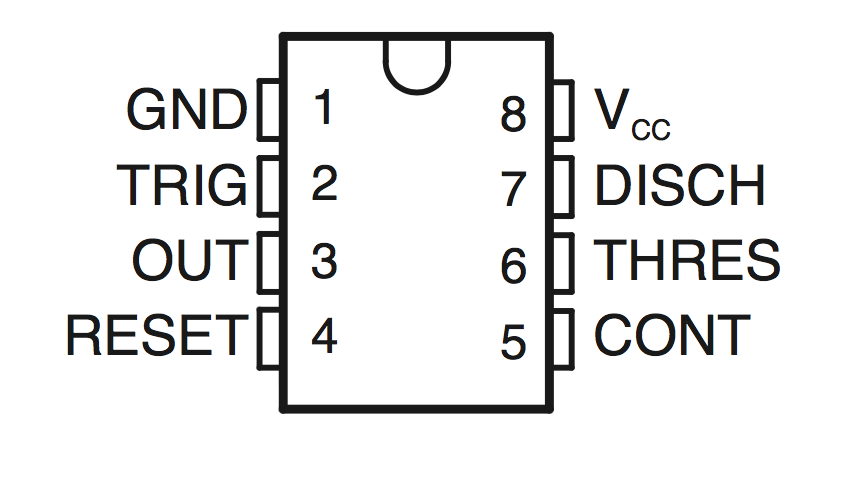
\includegraphics[height=7cm]{figures/2_4_4hastighedsmaal/komp555pin.png}
	\caption{Pindiagram over NE555P}
	\label{fig:komp555pin}
\end{figure}

\subsubsection{NPN-transistor - BC547}
Vi benyttede en NPN transistor til at forstærke signalet, da man ikke kan trække en særlig høj strøm fra en NOR gate. Vi ved dog at når der kommer over de \SI{0.7}{V} fra Base af transistoren, vil strømmen løbe fra collecter til emitter. Den er således "mættet" eller "aktiv". Et pindiagram kan findes på Figur \ref{fig:npntransistor}.
Databladet kan findes i kilde nr. \cite{NPNtransistorKomp}.

\begin{figure}[H]
	\centering
    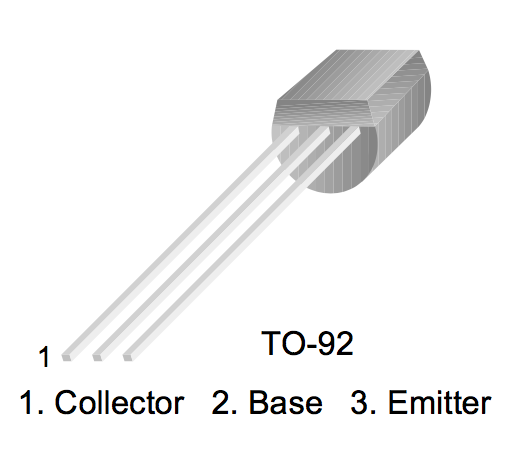
\includegraphics[width=7cm]{figures/2_4_4hastighedsmaal/kompNPNtransistor.png}
	\caption{Fra venstre mod højre 1. Collector, 2. Base, 3. Emitter. Kilde:\cite{NPNtransistorKomp} - side 1}
	\label{fig:npntransistor}
\end{figure}



\subsubsection{Signal invertering - HEF4001B}
Kilde: \cite{kompInverter}
Vi har benyttet komponenter HEF4001B som er en IC med OR gates, som vi benytter til at inverterer signalet fra 555-timeren.



% ----------- PIN DIAGRAM
\begin{figure}[H]
	\centering
    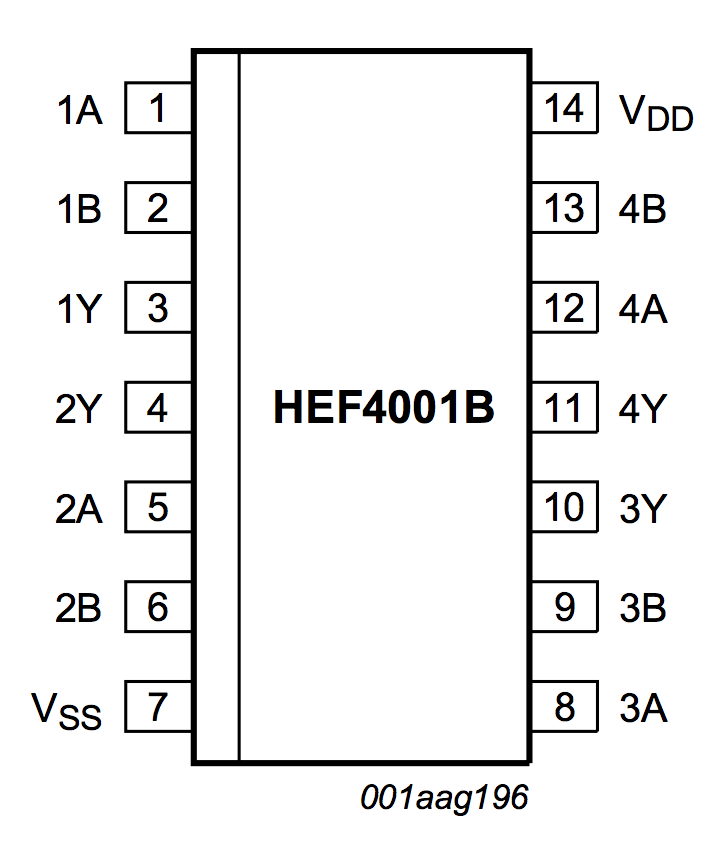
\includegraphics[height=7cm]{figures/2_4_4hastighedsmaal/kompInverterpin.png}
	\caption{Pindiagram over HEF4001B}
	\label{fig:kompInverter}
\end{figure}
% --------------


\subsubsection{Arduino}
Se afsnit \ref{sec:arduino}.

\subsection{Teori}
\subsubsection{Benyttelse af diode som variabel spænding}
\subsubsection{Nor-gate}
En norgate er en af de logiske gate der tager et digital signal som input og laver et nyt digitalt signal som output baseret på hvilke dens input. I vores tilfælde havde vi tænkt os at bruge en not gate til at invatere vores input. Men siden at det var nemmere at få fat på en nor-gate i stedet for en not gate har vi brugt den i stedet for og sat den ene inputpin til ground så den fungere ligesom en notgate.
\subsubsection{Hastighedsmålingsmetoder}
% \subsubsection{2 sensorer}
% \subsubsection{Knap og sensor}
Tidsmålingen bestemmes ved at vi kender et hvis strækning bolden har bevæget sig i, samt at man kender det tidsinterval bolden bevæger sig strækningen. Således bestemmes hastigheden:
\begin{align}
	v_{bold} &=\frac{\Delta s}{\Delta t} \\
\end{align}
 Heraf er der to løsninger til at bestemme dette.
Den ene er at benytte to infrarød afsender og modtagere kredse, som er sat sammen i par. Således at når den første del registrerer at en bold passerer undervejs så begyndes der at tage tid, indtil den næste del registrerer at bolden passerer. 

Den anden metode er at benytte en infrarød afsender og modtager-kreds og en knap, så når der trykkes på knappen tages der tid fra at bolden skydes af sted til at den registreres af infrarød afsender og modtager kreds.

Vi endte med at vælge den anden metode, grundet tidspres da vi efter vores fremstilling stødte på problemer, da kredsløbet ikke fungerede på PCB. Se afsnit \ref{subs:endeligProto}.
\todo{Hold øje med om der refereres til det rigtige afsnit}








\subsection{Beregninger}
\todo{mangler nogle enkelte beregninger}
\subsubsection{555 timer modstande} \label{calc:555timerResistance}
For 555 gælder det at vi ønsker en frekvens på 
\[
	f_{target} =  \SI{1000}{\hertz}
\]

Der kan opstilles 4 ligninger for 555 timeren således: 
For mark-time gælder det at
\begin{align}
	T_m &= 0.7 \cdot C_1 \cdot (R_1 + R_2) \label{eq:marktime} \\
\end{align}
For space-time gælder det at 
\begin{align}
	T_s &= 0.7 \cdot C_1 \cdot (R_2) \label{eq:spacetime} \\
\end{align}

For perioden gælder det at 
\begin{align}
	T &= \frac{1}{f} = T_s + T_m \label{eq:periodtime} \\
\end{align}
Og da dutycyclen skal være så tæt på $100$ som muligt sættes følgende forhold til at gælde
\begin{align}
	T_m &= 100 \cdot  T_s \label{eq:dutycycle} \\
\end{align}
Ved at løse ligningssystemet for ligningerne \ref{eq:spacetime}, \ref{eq:dutycycle}, \ref{eq:marktime}, \ref{eq:periodtime}, og isolerer for $R_1$ og $R_2$ og opskriver den som funktion af kapacitoren og frekvensen fås udtrykkende:
\begin{align}
	R_{1} \left( C_1,f \right) &= 1.400\,{\frac {1}{f \cdot C_1}} \\[2ex]
	R_{2} \left( C_1,f \right) &= 0.01414\,{\frac {1}{f \cdot C_1}}
\end{align}
Så antages at kondensatoren er 
\[
	C_1 = \SI{1.0d-6}{\farad}
\]
Da det antages vi bare benytter standardværdien. \todo{Er det standardværdien?***}

Frekvensen er nævnt og således bliver modstandende
\begin{align}
	R_1(\SI{1.0d-6}{\farad},\SI{1000}{\hertz})&= \SI{1400}{\ohm} \\[1ex]
	R_2(\SI{1.0d-6}{\farad},\SI{1000}{\hertz})&= \SI{14.14}{\ohm}
\end{align}

\subsubsection{Bestemmelse af modstande for peak-detektoren}

Vi har besluttet at benytte en peak-detektor til at opfange IR signalet til modtageren. Heraf benyttes der en simpel peak-detektor opbygning\todo{Er det den rigtige betegnelse***}.  Udtryk og teori benyttet er fra kilde \cite{peakdetectorCalc}.

Ud fra diodens karakteristika fås en forward-biased resistans på
\[
	r_{df} = \SI{607}{\ohm}
\]
og en reversed bias resistens på
\[
	r_{dr} = \SI{2d7}{\ohm}
\]
Således gælder det at vi skal vælge en modstand $R$ hvor det gælder at
\[
	r_{df} < R < r_{dr}
\]
Vores tidskonstant $\tau_2$ kan defineres som
\[
	\tau_2 = R \cdot C
\]
hvor $C$ er størrelsen på kapacitoren benyttet i peakdectoren.
Vi har besluttet at peaket skal være omtrent ved 
\[
	U_{peak} = \SI{4}{V}
\]
Og at differensområdet er på
\[
	\Delta U = \SI{0.5}{V}
\]
Vi beslutter at den modstand der benyttes i kredsen skal være på
\[
	R = \SI{56000}{\ohm}
\]
Vi regner med at få en frekvens på 
\[
	f= \SI{1000}{Hz}
\]
som vi prøver at tilnærme
% Deltaspænding er på 0.1 volt for at holde det nogenlunde konstant
Således hvis man skal opfylde følgende sammenhæng, må det gælde at:
\begin{align}
	\Delta U &= \frac{U_{peak}}{f \cdot t_2} \\
	\iff \Delta U &= \frac{U_{peak}}{ f \cdot R \cdot C}\\
	\iff C &= \frac{U_{peak}}{ f \cdot R \cdot \Delta U} \\
			&= \frac{\SI{4}{V}}{ \SI{1000}{Hz} \cdot \SI{56000}{\ohm} \cdot \SI{0.1}{V}} \\
			&= \SI{7.14d-7}{\farad}\\
			&\approx \SI{1}{\micro \farad}
\end{align}

Således skal vi benytte en kondensator til peakdetectoren på \SI{1}{\micro\farad}


\subsection{Test}
\todo{Der skal nok referes til billeder og navne på komponenter i billedet når der snakkes om tests***} 
\subsubsection{Afsender dioden}
Vi testede 555-timeren med et PC-oscilloskop.

På Figur ~\ref{fig:555noninv} er der en graf af den 555-timerens output, som det fremgår på info-boksene er duty cyclen er høj som beregnet. Det bemærkes også at frekvensen er lidt større end $\SI{1000}{Hz}$ men vi forventer ikke det giver os problemer.

Det inverterede signal kan ses på \ref{fig:555inv} og det fungerer som ønsket.
\begin{figure}[H]
	\centering
    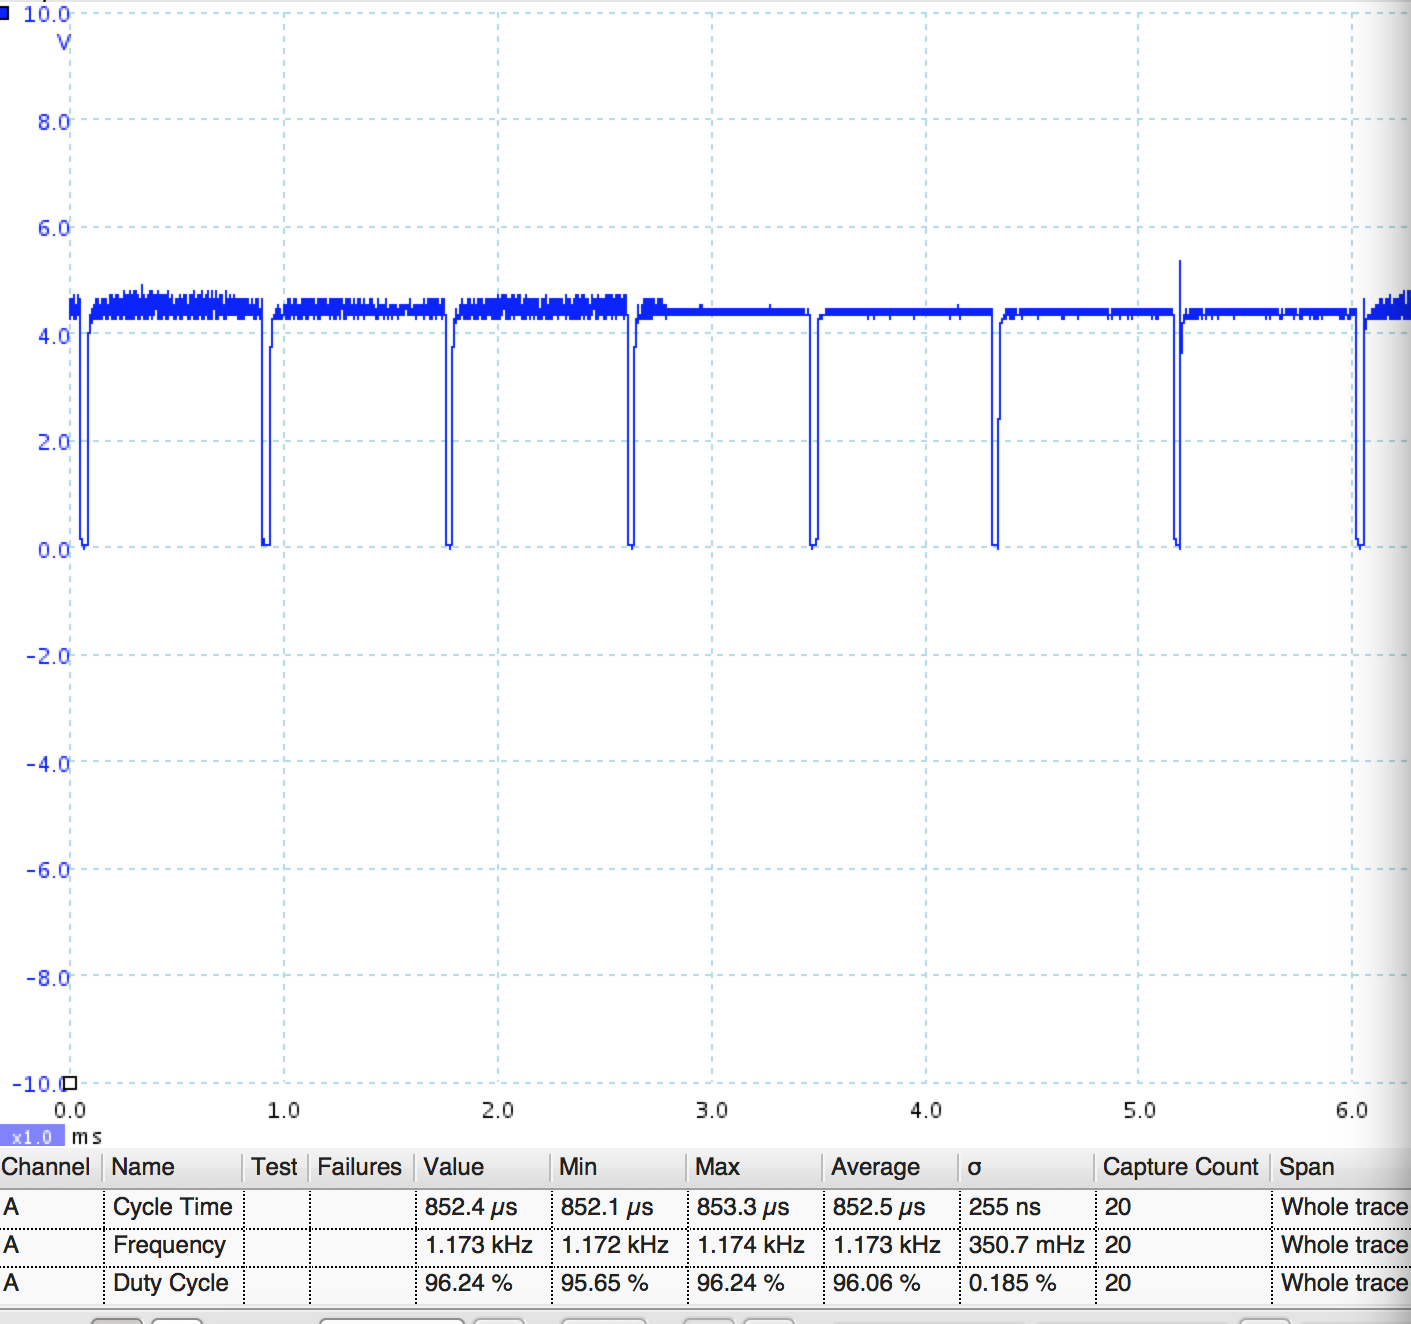
\includegraphics[width=13cm]{figures/2_4_3hastighed/555signal.png}
	\caption{Spænding som funktion af tiden med info-bokse i bunden}
	\label{fig:555noninv}
\end{figure}

\begin{figure}[H]
	\centering
    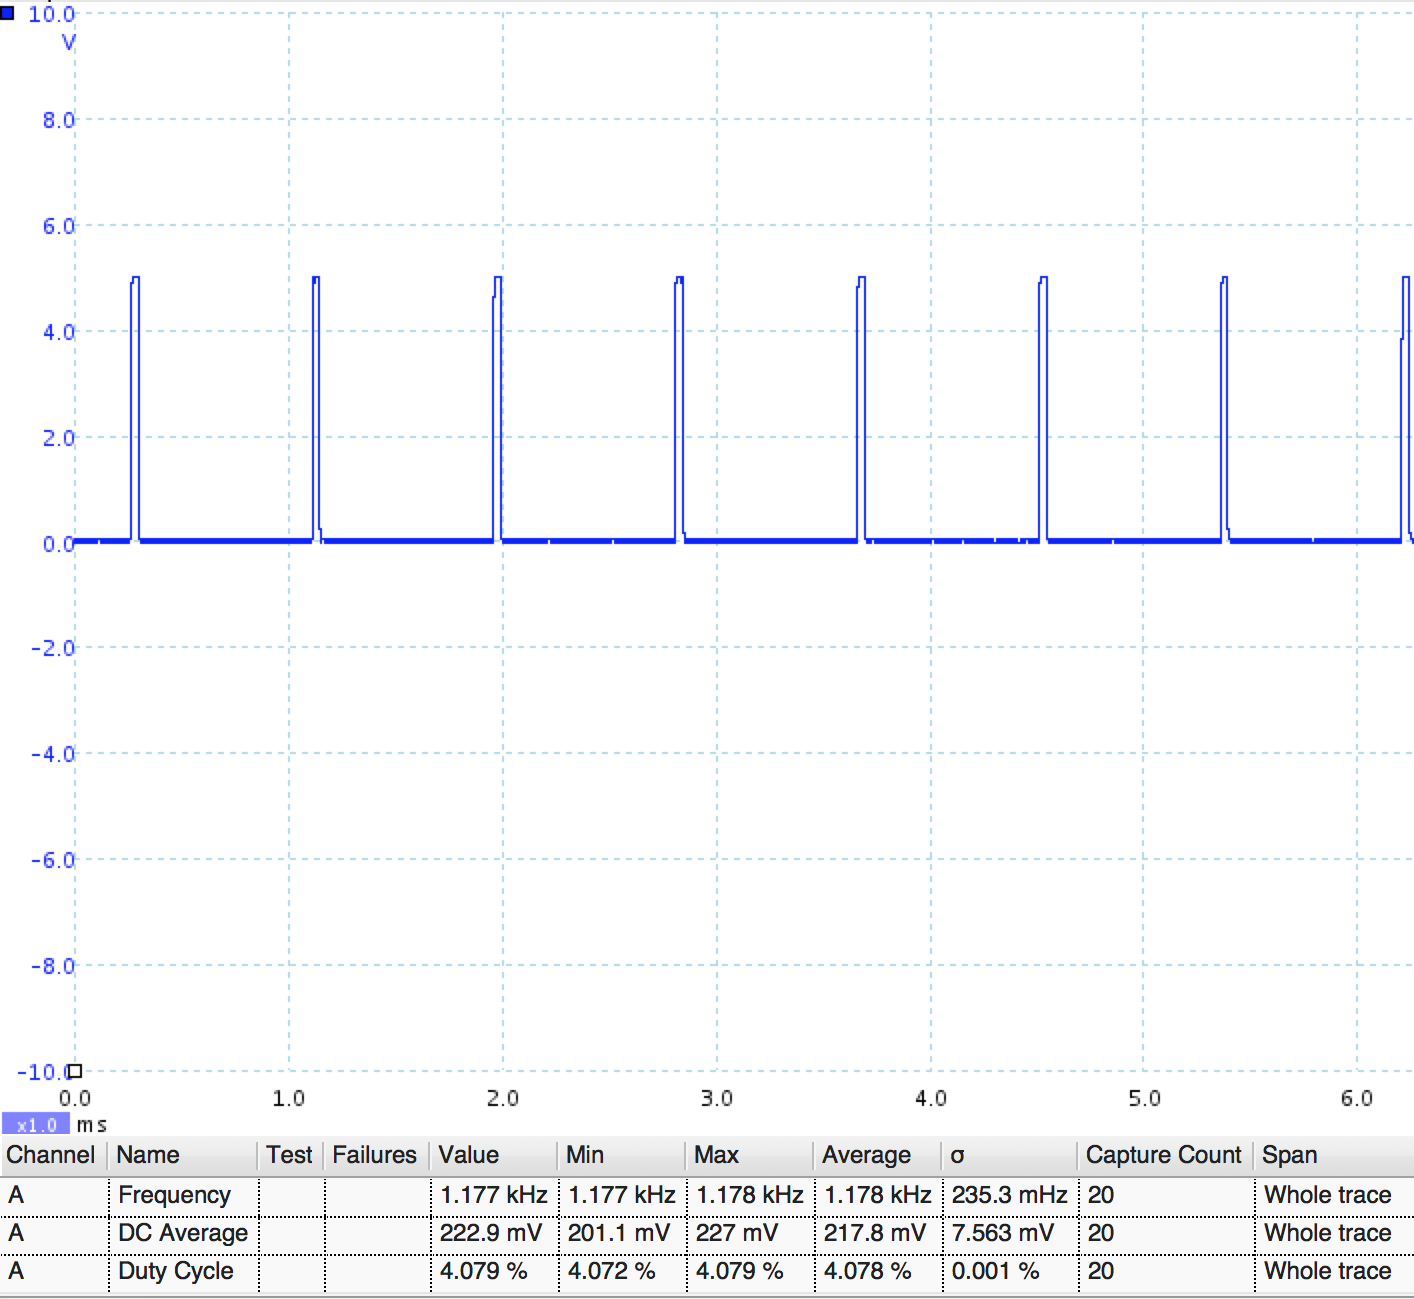
\includegraphics[width=13cm]{figures/2_4_3hastighed/555signalinv.png}
	\caption{Det inverterede signal som funktion af tiden med info-bokse i bunden}
	\label{fig:555inv}
\end{figure}

\begin{figure}[H]
	\centering
    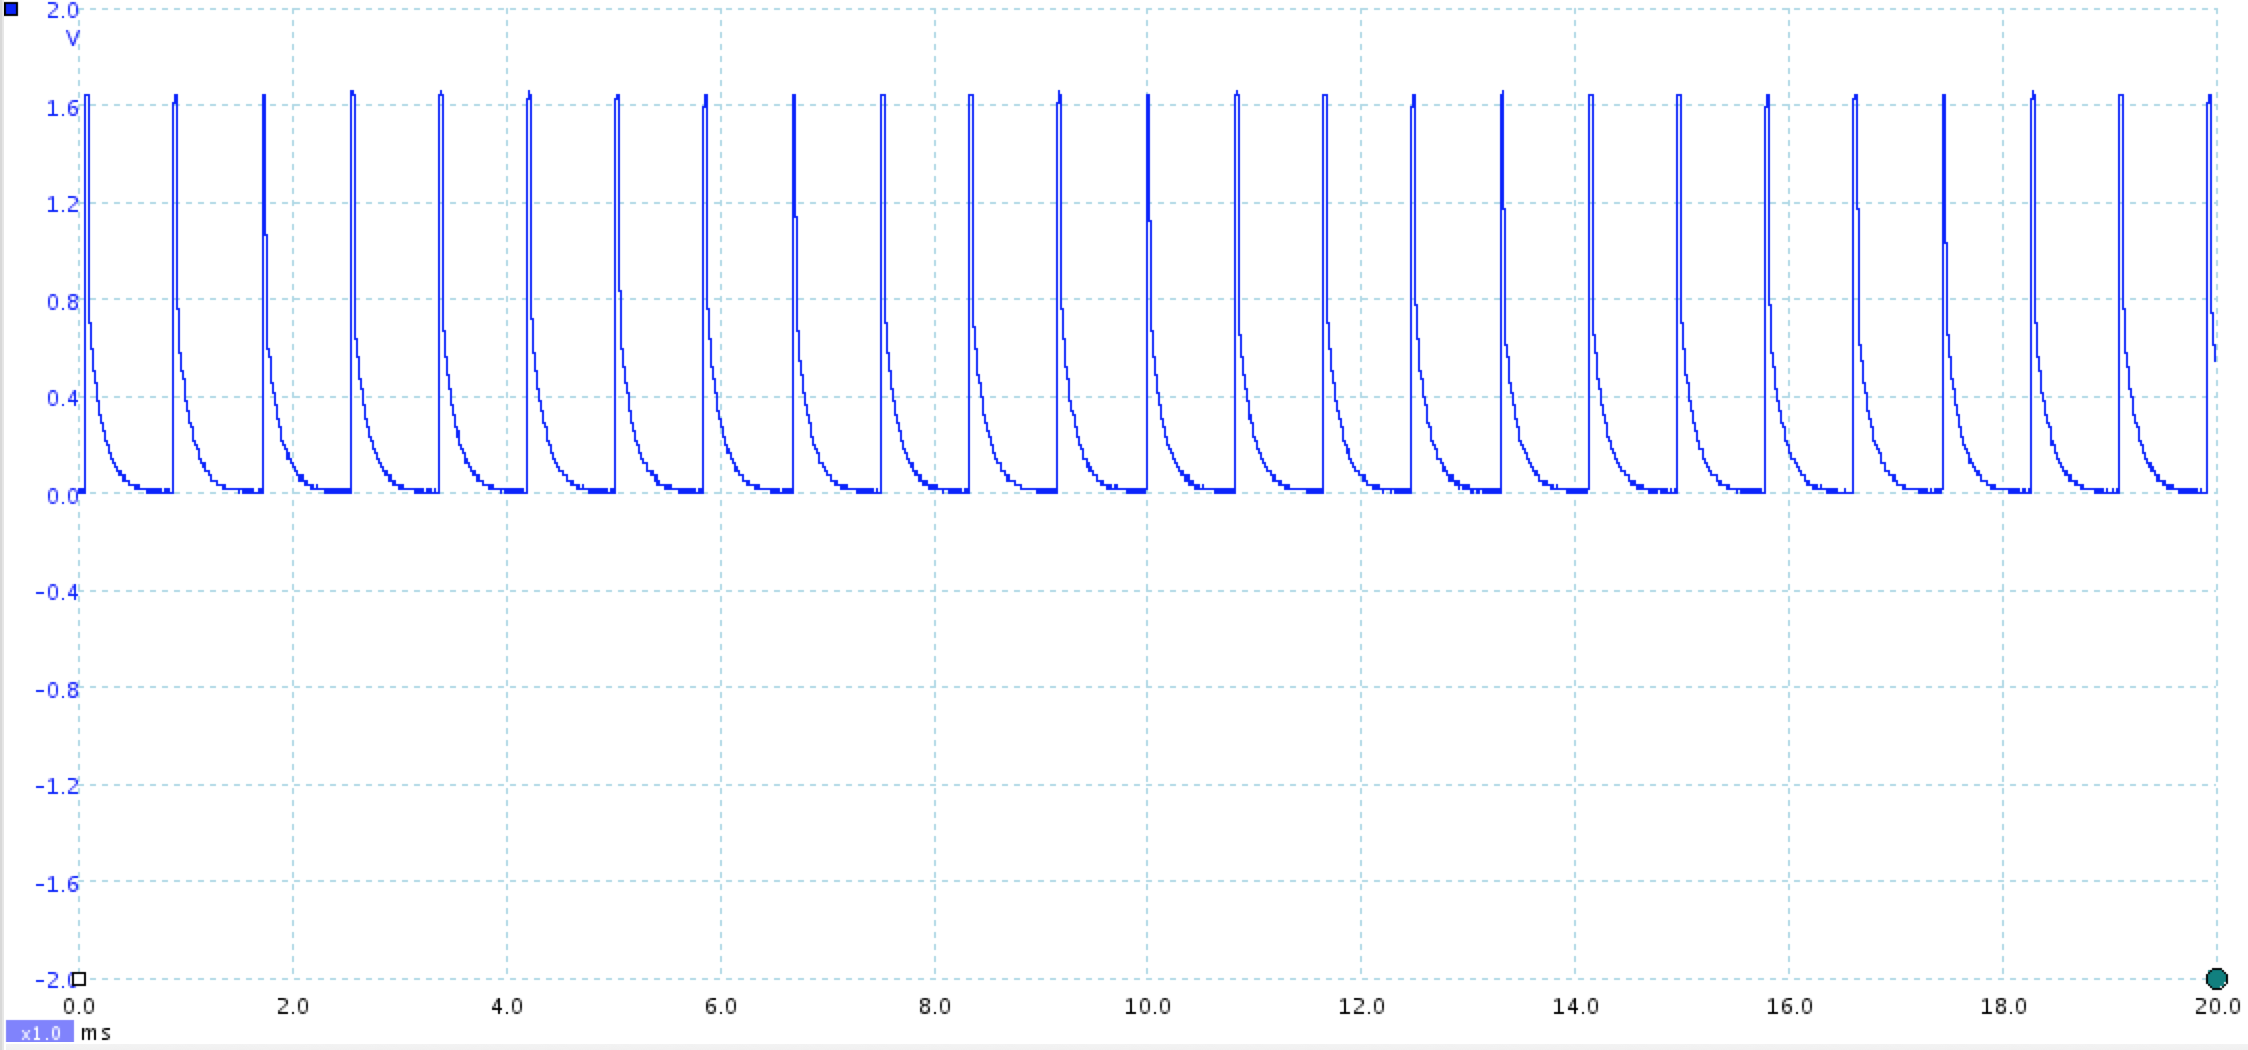
\includegraphics[width=13cm]{figures/2_4_3hastighed/555timerDiode.png}
	\caption{Spænding over dioden som funktion af tiden}
	\label{fig:diodeafsender}
\end{figure}
% 12/(10*10^(-3))
Spændingen over dioden kan ses på Figur ~\ref{fig:diodeafsender}.
Frekvensen estimeres ud fra de 12 første bølgetoppe. Heraf bemærkes at 

\[
	f_{diode} \approx \frac{12}{\SI{10d3}{s}} = \SI{1200}{Hz}
\]
Hvilket svarer fint til frekvensen af outputtet fra 555-timeren.

\subsubsection{Modtager dioden} \label{subs:modtagertest}
For modtager-delen af kredsen fremgår det på \ref{fig:IR_modtagerTest} at frekvensen er omtrent $\SI{1.4d3}{Hz}$, og et tydelig spændingsforskel på omtrent $-\SI{5}{V}$ hvilket er et fint og tydeligt signal. Dog afviger frekvensen væsentlig fra vores ønskede frekvens, men vi regner ikke med at det giver problemer med hensyn til udformningen af produktet.
\todo{vi kunne muligvis godt have mere tekst her}
\begin{figure}[H]
	\centering
    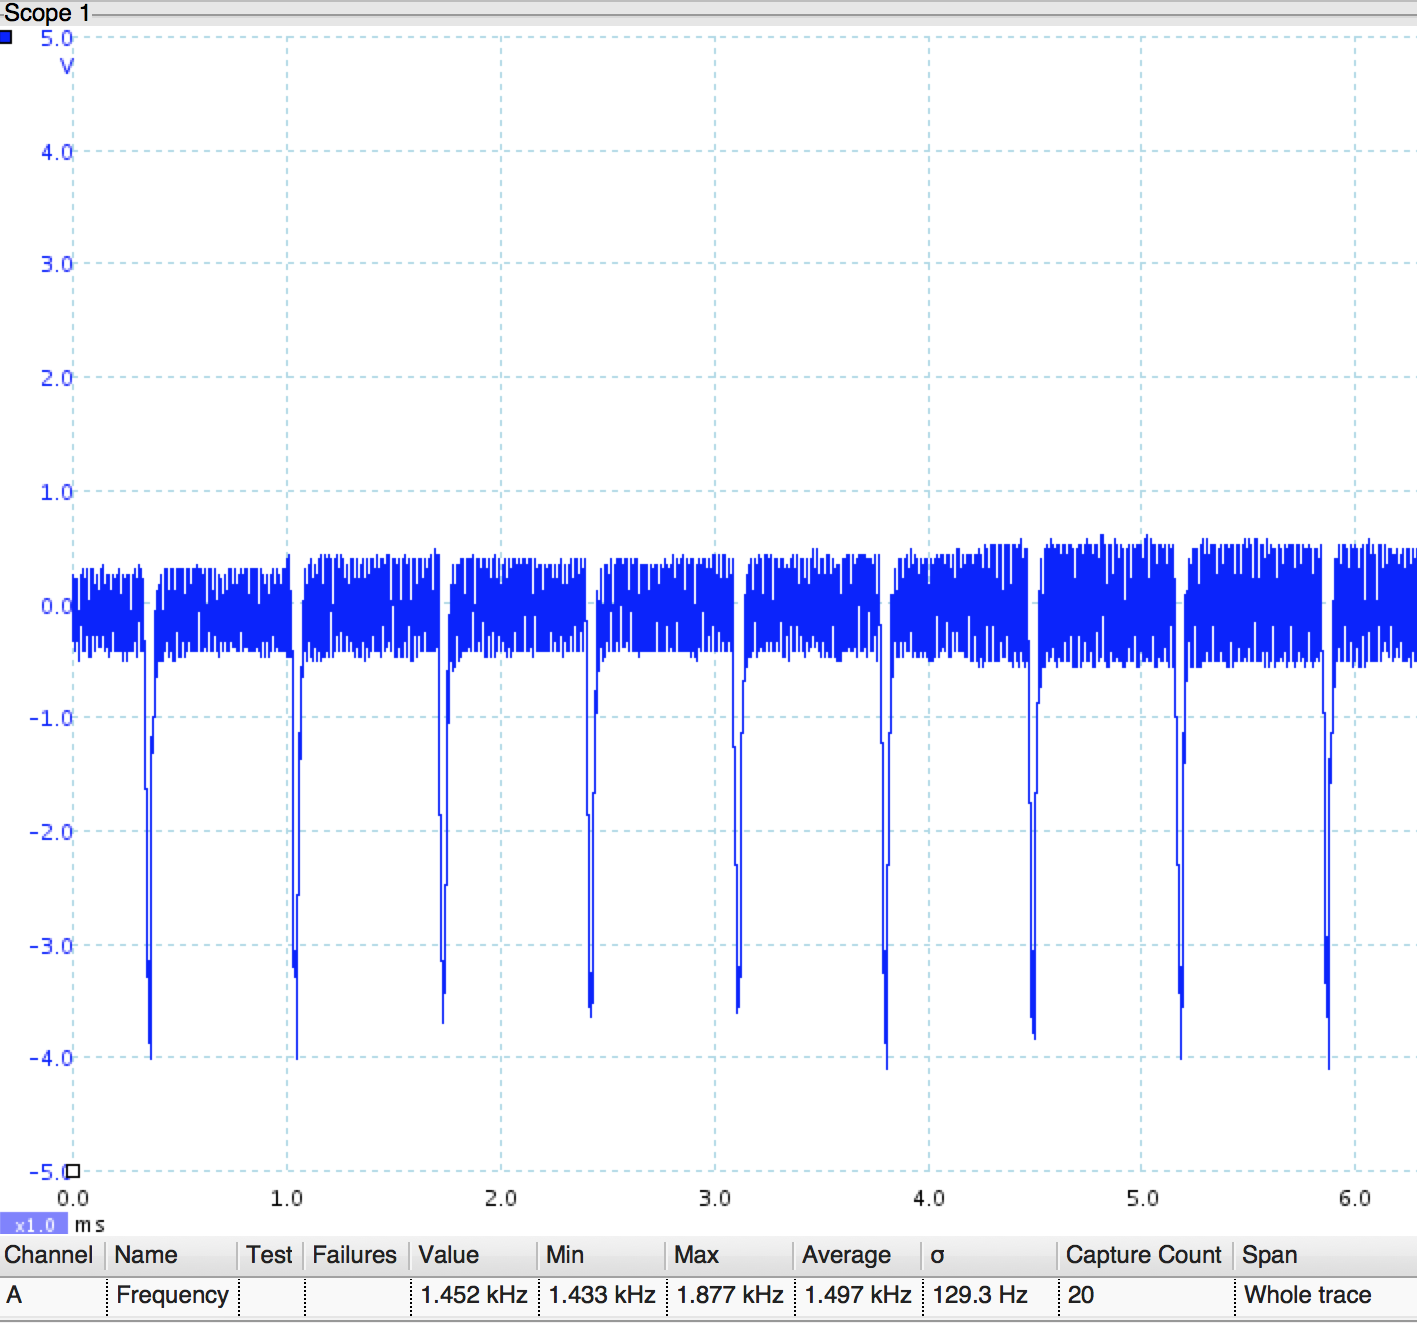
\includegraphics[width=13cm]{figures/2_4_3hastighed/IR_modtager.png}
	\caption{Spændingen som funktion af tiden af modtagerkredsens signal}
	\label{fig:IR_modtagerTest}
\end{figure}


















\section{Controller}
\begin{figure}[H]	
	\centering
    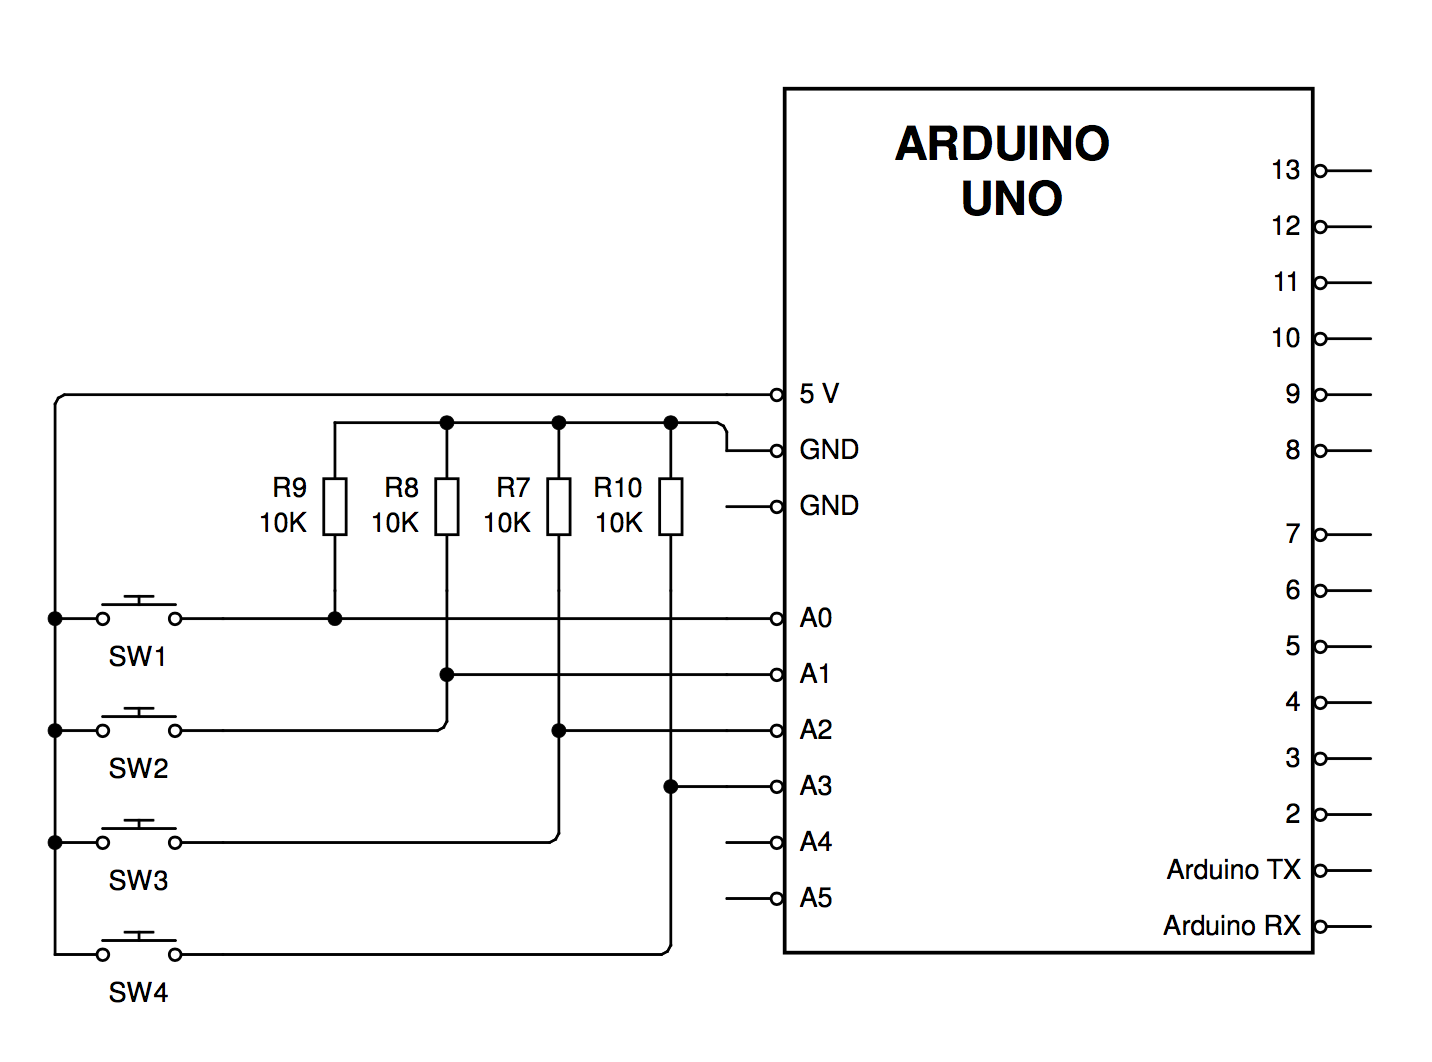
\includegraphics[width=13cm]{figures/CIRCUITS/controllerFinal.png}
	\caption{Et billede af kredsløbet for controller kredsen.}
	\label{kreds:controller}
\end{figure}

\subsection{Komponenter}
I kontrolleren bliver der kun brugt simple fysiske switches, modstande og en Arduino. Se afsnit \ref{sub:arduino} for beskrivelse af Arduino.


\subsection{Teori}
For at undgå en kortslutning bliver der sat en modstand imellem den ene switch side og ground. På den anden side a switchen er der $\SI{5}{V}$.
%\subsection{Beregninger}

%\subsection{Test}
\section{Display}

\subsection{LCD-kredsløb}
%%%%%BILLEDE AF KREDSLØB
\begin{figure}[H]
	\centering
    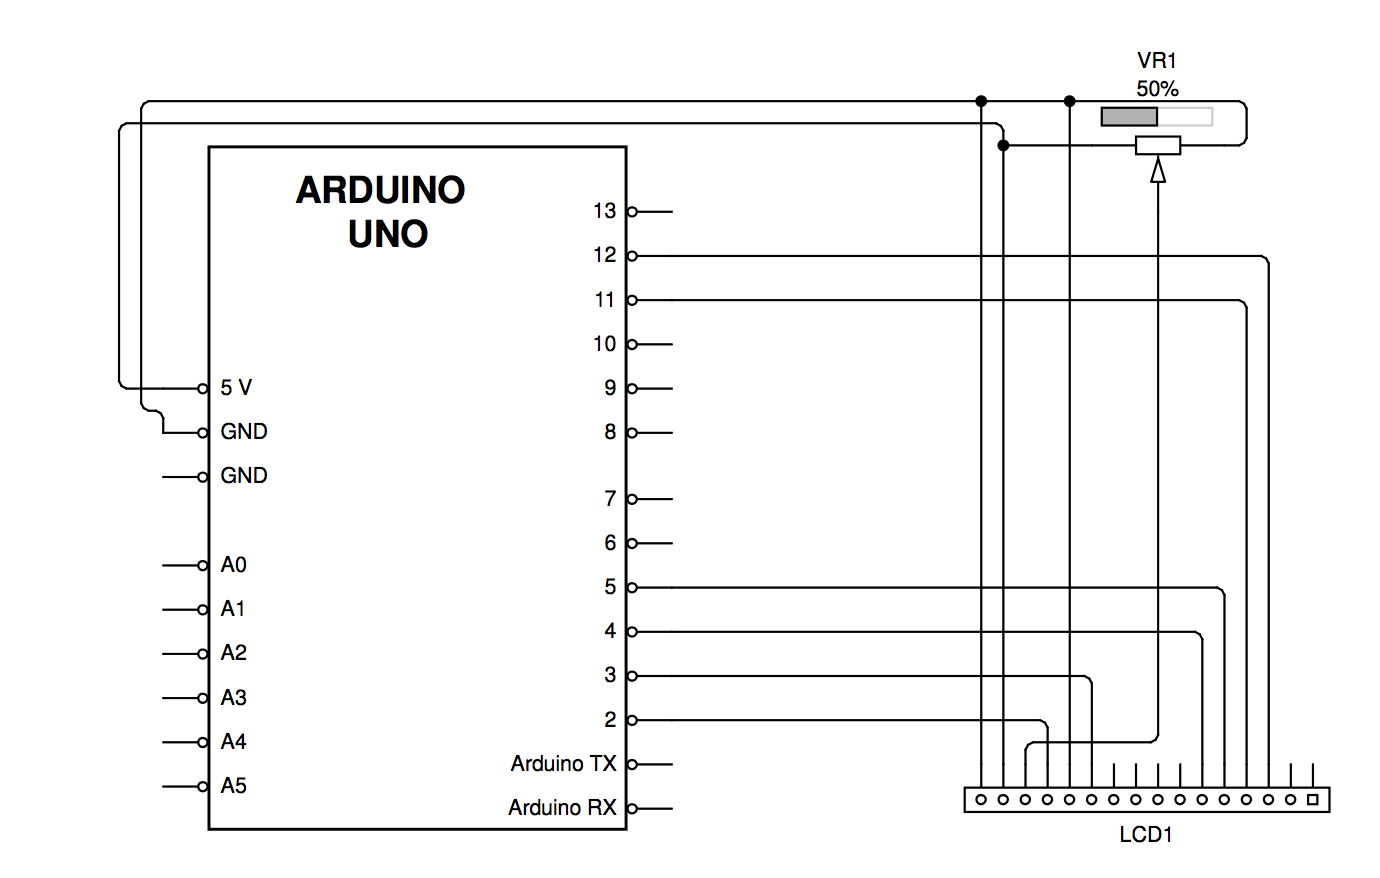
\includegraphics[height=10cm]{figures/CIRCUITS/LCDFinal.png}
	\caption{Arduino LCD kreds lavet ud fra arduino siden, se \cite{arduinoLCD}}
	\label{arduinoLCD}
\end{figure}
\subsubsection{LCD setup}
Vi benytter et LCD display, da det let kan forbindes direkte til arduioen uden et ekstra interface ved brug af LiquidCrystal biblioteket. Biblioteket vi benytter gør brug af ASCII kode se figur ~\ref{ASCII} til at vise symboler på et display.
Vi benyttede et 4-bit datainterface setup (se \cite{arduinoLCD}), hvor displayet skriver på to linjer.


\subsection{Komponenter}
% ************** kilde

% Skriv om displayet og displaydriveren
\subsubsection{LCD display}
LCD displayet vi benyttede havde en indbygget controller som vist på Figur ~\ref{driver}.
\begin{figure}[H]
	\centering
    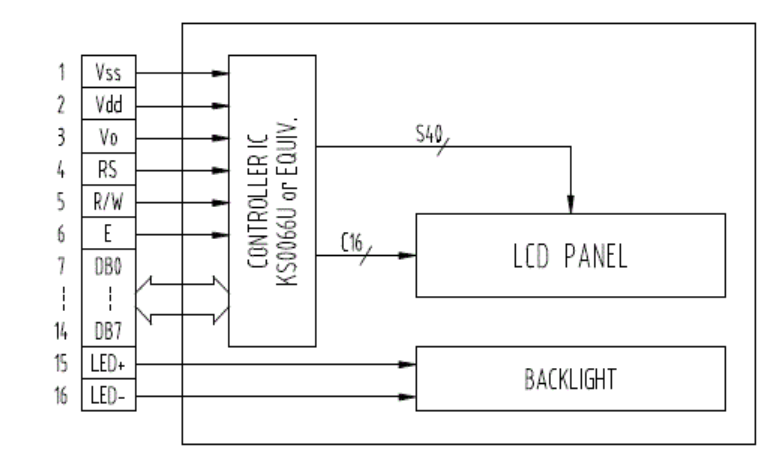
\includegraphics[width=10cm]{figures/LCDdesign/displayblokdiagram.png}
	\caption{Et blok diagram over databen og kontrolben til  kontroller, backlight, LCD panel. Kontrolleren er indbygget i displayet. kilde: [Uddrag fra projektvejledning]}
	\label{driver}
\end{figure}
\subsubsection{Arduino}
Se afsnit \ref{sec:arduino} 


% Skriv om teori. Skriv om 4-bit interface
\subsection{Teori}
\subsubsection{LiquidCrystal library}
LiquidCrystal library bruger vi til at kunne få arduinoen til at sende den ønskede tekst af f.eks. af en måling til et LCD. LiquidCrystal gør brug af ASCII tegnsæt til at tolke binære signaler til tekst. Et uddrag på ASCII karakterer kan ses på Figur ~\ref{ASCII}. 
\begin{figure}[H]
	\centering
    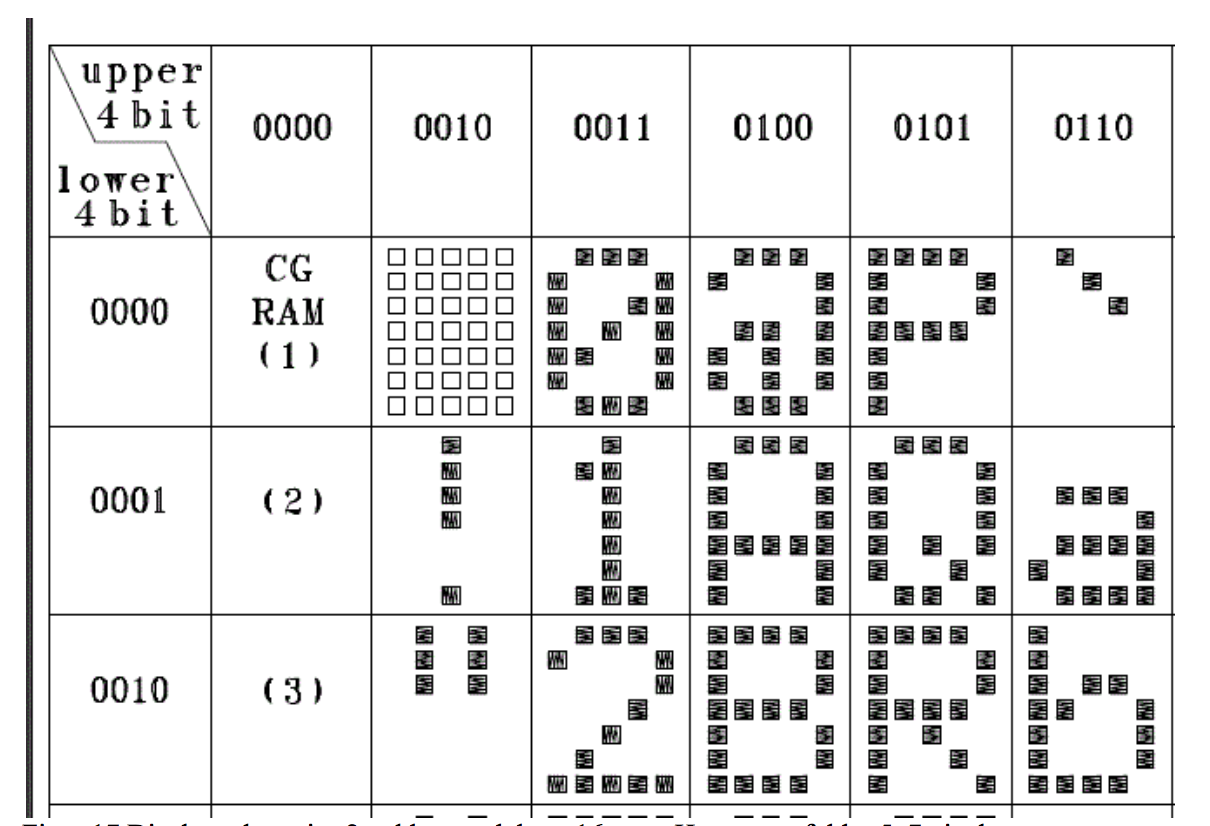
\includegraphics[width=10cm]{figures/LCDdesign/ASCII.png}
	\caption{Et eksempel på nogle ASCII koder benyttet af LiquidCrystal library - kilde: [Uddrag fra projektvejledning]}
	\label{ASCII}
\end{figure}

\todo{Skriv om ASCII}

 
\subsection{Test}
Vi benyttede en simpel "Hello World" program til at teste skærmen, koden fik vi fra \cite{arduinoLCD}.





% Begin CODE EXAMPLE
% ---------------------------
\begin{lstlisting}[caption=kodeeksempel "Hello World" med timer, label={alg:helloworld}]
// Inkluder koden fra liquidcrystal library:
#include <LiquidCrystal.h>

//Initialiser biblioteket 
//med disse interfacepins.
LiquidCrystal lcd(12, 11, 5, 4, 3, 2);

void setup() {
//Bestemmer antallet af hhv.
//kolonner og rækker for displayet
  lcd.begin(16, 2);
//Printer besked til displayet
  lcd.print("hello, world!");
}

void loop() {
// Sætter cursor til at være på anden række,
// som er markeret 1.
  lcd.setCursor(0, 1);
//Printer antallet af sekunder der 
//er gået siden reset.
  lcd.print(millis() / 1000);
}
\end{lstlisting}
% ----------------------------------
% End code example


Potentiometret kunne justerer skærmens styrke fint.

\section{Ladningssensor}
\begin{figure}[H]
	\centering
    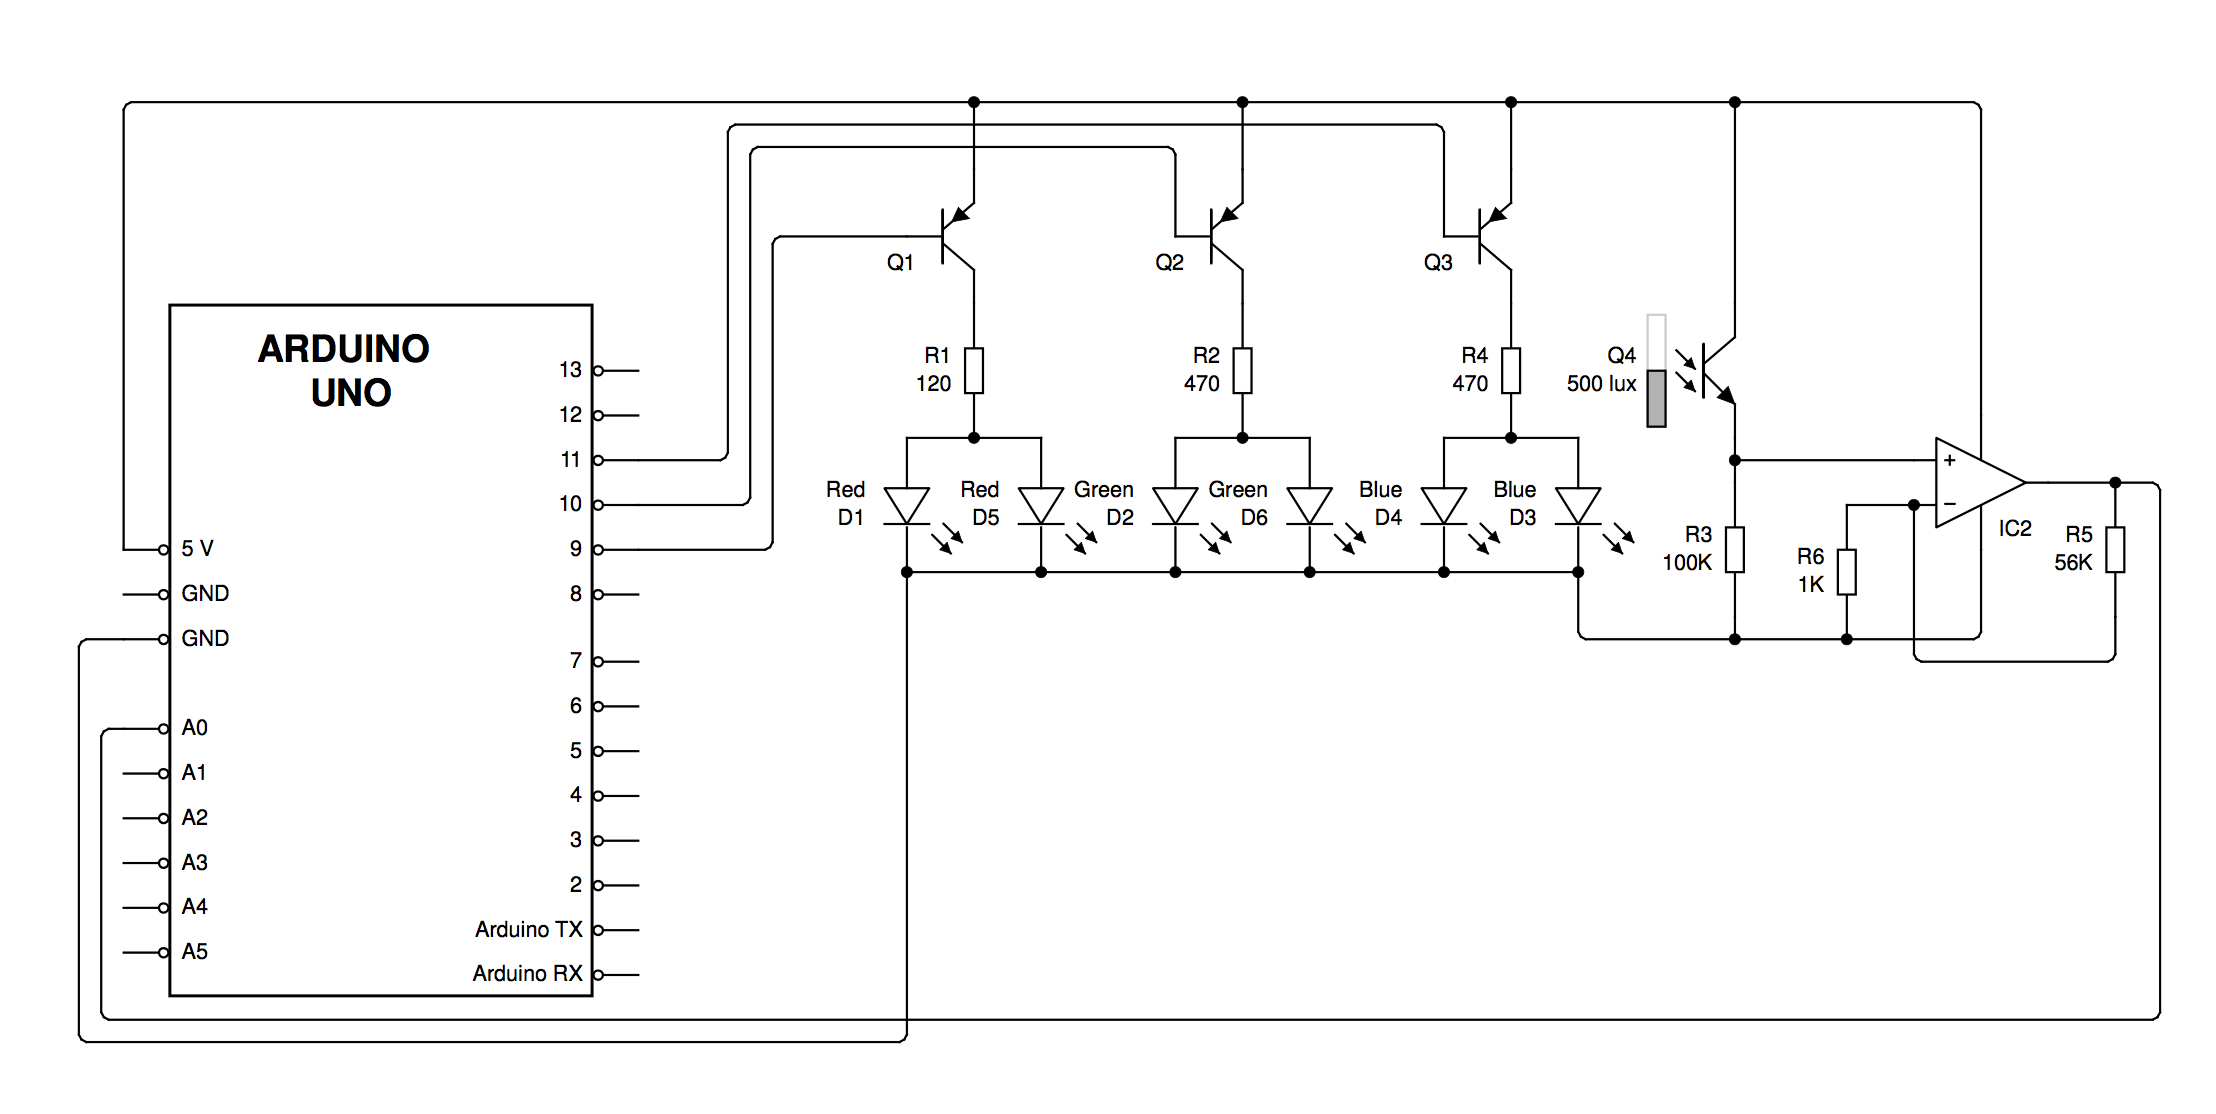
\includegraphics[width=\textwidth]{figures/CIRCUITS/farvesensorFinal.png}
	\caption{Et billede af kredsløbet for ladningssensor kredsen.}
\end{figure}

\subsection{Komponenter}
\subsubsection{BPW21 - Fotodiode}
\begin{figure}[H]
	\centering
    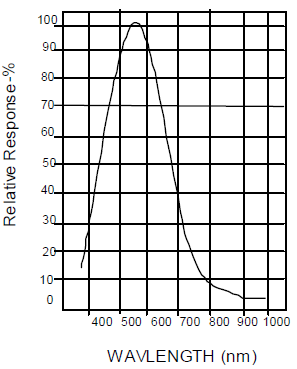
\includegraphics[height=10cm]{figures/komponenter/photosensor}
	\caption{Normal speltral respons angivet i procent}
	Se databladet i kilde \cite{kompPhoto}.
\end{figure}
BPW21 er en fotodiode, som betyder at det er en diode som omdanner lys til elektrisk strøm. \todo{skriv teori om BPW21}

\subsubsection{LED - RGB WHITE DIFFUSED LENS COMMON CATHODE}
\begin{figure}[H]
	\centering
    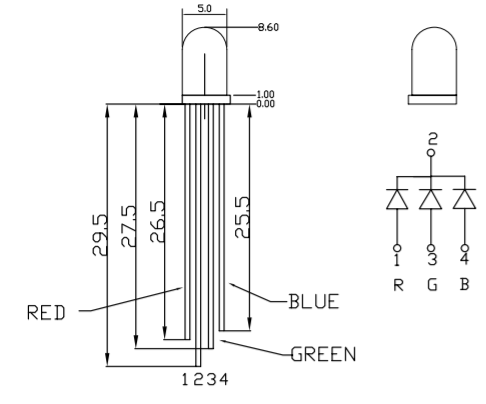
\includegraphics[height=7cm]{figures/komponenter/LED2}
	\caption{Diagram af LED'en}
	Se databladet i kilde \cite{kompRGBLED}.
\end{figure}
\begin{figure}[H]
	\centering
    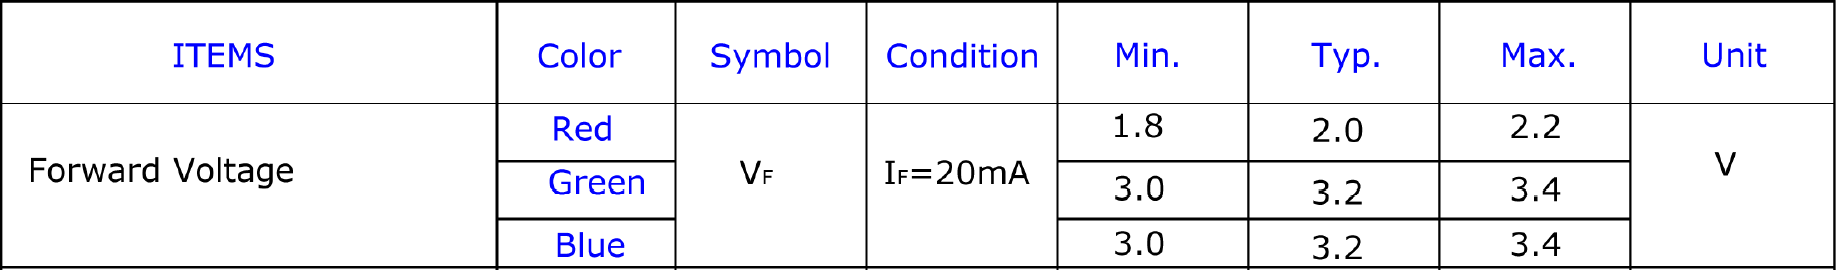
\includegraphics[width=\textwidth]{figures/komponenter/LED}
	\caption{Spændingsfaldet over de forskellige LED'er}
	Se databladet i kilde \cite{kompRGBLED}.
\end{figure}
Vi benytter en LED som kan lyse i 3 forskellige farver, rød, grøn og blå. Vi benyttede en LED med en fælles katode. Dette betyder at vi kan koble LED'ens katode til jord, også styre spændingen sat på hver af deres anoder. For ikke at trække for meget strøm fra arduinoen, benytter vi en NPN transistor som kontakt til LED'erne.

\subsubsection{NPN transistor}
\todo{Skriv om NPN transistor}

\subsubsection{OP Amp - MCP601}
\begin{figure}[H]
	\centering
    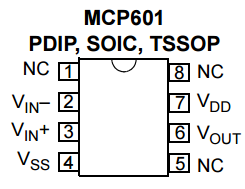
\includegraphics[width=7cm]{figures/komponenter/OPAMP}
	\caption{Bendiagram af MCP601}
	Se databladet i kilde \cite{kompOPAMP}.
\end{figure}

\subsection{Teori}
\subsubsection{OP Amp}
%%---------- indsæt billede---------------------------------%

En operationsforstærker (OP Amp) er en type forstærker der tager imod to inputs, inverting input voltage ($V_{in-}$) og non-inverting input voltage ($V_{in+}$). Outputtet fra en operationsforstærker  ($V_{out}$), kan beskrives med formlen
\begin{align}
V_{out}&=A(V_{in+}-V_{in-})\quad,\quad V^- \leq V_{out}\leq V^+ 
\end{align}
Her er $A$ den elektriske gain af operationsforstærkeren. $A$ er som reel omkring $10^5$ til $10^6$, men man anser den som at gå imod uendelig. Vi benyttede os af en non-inverting amplifier. 
\begin{figure}[H]
	\centering
    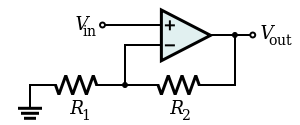
\includegraphics[width=\textwidth]{figures/komponenter/NonInvAmp}
	\caption{El diagram for non-inverting amplifier}
	\label{fig:noninvamp}	
\end{figure}
Som man kan se ud fra el diagrammet \ref{fig:noninvamp}, er der en spændingsdeler imellem $V_{out}$ og $V_{in-}$. Vi ved at for en spændingsfordeler gælder der
\begin{align}
U_{out}&=U\cdot \frac{R_2}{R_1+R_2}
\end{align}
Hvor at $U_{out}$ er spændingen over $R_2$ og $U$ er spændingen over $R_1$ og $R_2$.
Dette betyder at
\begin{align}
V_{in-}&=V_{out}\cdot \frac{R_2}{R_1+R_2}
\end{align}
Hvis vi indsætter dette i vores udtryk for $V_out$ gælder der
\begin{align}
V_{out}&=A(V_{in+}-V_{in-})\quad,\quad V^- \leq V_{out}\leq V^+\\
V_{in-}&=V_{out}\cdot \frac{R_2}{R_1+R_2}\\
\rightarrow V_{out}&= A(V_{in+}-V_{out}\cdot \frac{R_2}{R_1+R_2})\\
\rightarrow V_{out}+A\cdot V_{out}\cdot \frac{R_2}{R_1+R_2}&=A\cdot V_{in+}\\
\rightarrow V_{out}(1+A\cdot \frac{R_2}{R_1+R_2})&=A\cdot V_{in+}\\
\rightarrow V_{out}&=\frac{A\cdot V_{in+}}{1+A\cdot \frac{R_2}{R_1+R_2}}\\
\end{align}
Da $A$ er et meget højt tal, så kan $1$ i nævneren negligeres.
\begin{align}
V_{out}&=\frac{A\cdot V_{in+}}{A\cdot \frac{R_2}{R_1+R_2}}\\
&=\frac{V_{in+}}{\frac{R_2}{R_1+R_2}}\\
V_{out}&=V_{in+}\cdot(\frac{R_1}{R_2}+1)\\
\rightarrow \frac{V_{out}}{V_{in+}}&=\frac{R_1}{R_2}+1
\end{align}
Dette udtryk kan vi benytte til at beregne forstærkningen af vores non-inverting amplifier.
(Kilde: Teknik A - OP-amp DC-kobling (teori udleveret af læreren uden yderligere kildeangivelse))
\subsubsection{Analog input til registrering af farve}
Arduinoens analog input er beskrevet i afsnit \ref{sec:ard:analog}. Vi benytter denne funktion til at få outputtet fra vores farvesensor ind i arduinoen.
\subsection{Beregninger}
\subsubsection{Modstanden af LED}
Ifølge \cite{kompLED} gælder det for LED'en at dens typiske spænding for den blå og grønne LED
\[
	V_{GB typisk} = \SI{3.2}{V}
\]
Og for den røde 
\[
	V_{R typisk} = \SI{2}{V}
\]
Og kan klare en strømstyrke på
\[
	I = \SI{20d-3}{A} 
\]
Ud fra ohms lov må det betyde at hvis indgangsspændingen er på $\SI{5}{V}$, at modstanden til de enkelte LEDer skal være
\begin{align}
	R&= \frac{U}{I}\\
	R_{RLED} &= \frac{\SI{5}{V}-\SI{2}{V}}{\SI{2.0d-2}{A}} = \SI{150}{\ohm}\\
	R_{GLED} &= \frac{\SI{5}{V}-\SI{3.2}{V}}{\SI{2.0d-2}{A}} = \SI{90}{\ohm}\\
	R_{BLED} &= \frac{\SI{5}{V}-\SI{3.2}{V}}{\SI{2.0d-2}{A}} = \SI{90}{\ohm}\\
\end{align}
Ud fra dette valgte vi at benytte modstandene 
\begin{align}
	R_{RLED} &= \SI{180}{\ohm}\\
	R_{GLED} &= \SI{100}{\ohm}\\
	R_{BLED} &= \SI{100}{\ohm}\\
\end{align}
Det vidste sig dog at en LED ikke lyste nok op, og derfor satte vi en ekstra parallelt med den anden som vist på kredsløbstegningen. Dette betød at vi skulle beregne vores modstande igen. For en parallelforbindelse gælder
\begin{align}
\frac{1}{R_{tot}}&=\frac{1}{R_1}+\frac{1}{R_2}+...+\frac{1}{R_n}
\end{align}
hvor at der er $n$ parallelle modstande, som ønskes at erstattes med en samlet modstand $R_{tot}$. Da hver af de parallelle modstande, var de modstanden beregnet før, må den nye samlede modstand for hver farve være
\begin{align}
R_{R-tot}&=\frac{1}{\frac{1}{R_{RLED}}+\frac{1}{R_{RLED}}}\\
&=\frac{1}{\frac{1}{\SI{180}{\ohm}}+\frac{1}{\SI{180}{\ohm}}}\\
&=\SI{90}{\ohm}\\
R_{G-tot}&=\frac{1}{\frac{1}{R_{GLED}}+\frac{1}{R_{GLED}}}\\
&=\frac{1}{\frac{1}{\SI{100}{\ohm}}+\frac{1}{\SI{100}{\ohm}}}\\
&=\SI{50}{\ohm}\\
R_{B-tot}&=\frac{1}{\frac{1}{R_{BLED}}+\frac{1}{R_{BLED}}}\\
&=\frac{1}{\frac{1}{\SI{100}{\ohm}}+\frac{1}{\SI{100}{\ohm}}}\\
&=\SI{50}{\ohm}
\end{align}
Da vi havde beregnet de minimum modstande vi kunne bruge, prøvede vi os frem for at finde modstande, så hver LED lyste lige stærkt. Vi kom frem til disse modstande
\begin{align}
	R_{R-tot} &= \SI{120}{\ohm}\\
	R_{G-tot} &= \SI{470}{\ohm}\\
	R_{B-tot} &= \SI{470}{\ohm}\\
\end{align}
Her blev der lavet en test, af indgangsspændingen til Arduinoen, når der blev lyst med forskellige farver, på materialer med forskellig farve. Testen kan findes i tabel \ref{tab:farveudenforstaerker}.

\subsubsection{OPAMP modstande} \label{subs:opampanalog}
Vi besluttede os for at benytte en OPAMP, da vores største signal fra test 1 (se \ref{tab:farveudenforstaerker}) var på $\SI{0.06}{V}$, hvis man ser bort fra når alle lyser. Da vores precision af analog inputtet på arduinoen er omkring $\SI{0.005}{V}$ (se \ref{sec:ard:analog}), er disse udsving for små til at med sikkerhed kunne identificere farver. Vi benytter derfor en OPAMP, så det er nemmere at identificere hvilken farve der bliver brugt.
% R_in = 1k
% R_f = 56k
Vi valgte at den maksimale indgangsspænding til OPAMPen er
\[
	V_{in+} = \SI{0.08}{V}
\]
Vi ønsker at dette skal være det maksimale som Arduinoen kan måle ($\SI{5}{V}$)
\[
	V_{out} \approx \SI{5}{V}
\]
Heraf er den ønskede forstærkning
\[
	A_{target} = \frac{V_{out}}{V_{in+}} = \frac{\SI{5}{V}}{\SI{0.08}{V}}=62.5
\]

Denne forstærkning er ret høj og vi benytter derfor en non-inverting amplifier.

Vi bestemmer en rimelig værdi til den ene modstand er
\begin{align}
	R_{2} = \SI{1000}{\ohm} \label{eq:RinFarveOpAmp}
\end{align}
Og udtrykket for forstærkningen er

\begin{align}
	A_{target} = 1+\frac{R_1}{R_2} \label{eq:AtargetFarveOpAmp}
\end{align}
Ved at isolerer $R_1$ i ligningerne \ref{eq:RinFarveOpAmp} og \ref{eq:AtargetFarveOpAmp} fås
\[
	R_1 = \SI{61.5d3}{\ohm}
\]
Da vi ikke har denne modstand direkte, vælger vi at benytte en $\SI{56d3}{\ohm}$ modstand i stedet. Hvilket giver os en reel forstærkning på
\[
	A_{reel} = 1 + \frac{\SI{56d3}{\ohm}}{\SI{1000}{\ohm}} = 57	
\]
Hvilket svarer til et outputsignal på
\[
	V_{out} = \SI{0.08}\cdot 57 = \SI{4.56}{V}
\]
Hvilket er tilnærmelsesvis hvad vi gerne vil have. Derefter kørte vi den samme test som før vi havde forstærket signalet. Resultaterne kan ses i tabel \ref{tab:farvemedforstaerker}.





**** NOTER ****
Men da vi satte tre modstande ændrede vi det til ***. 
% MISC LED
Skriv LED anode eller cathode og indsæt tegning 
Simon → Farvesensor
Skriv om bestemmelse af modstande til LED
Start ->
G=100
B=100
R=180

Ændring ->
R=120
G=470
B=470

Skriv om arduino precision (10 bit)-> grunden til brug af opamps

Skriv om opAMP


Nævn af billederne i bilag (grøn blå) blev taget før at afstanden blev ændret fra 6 cm til 3cm.
(afstand 2 cm, mørklagt kasse)
% \usepackage[normalem]{ulem}
% \useunder{\uline}{\ul}{}

*************
\subsection{Test}
Vores teste foregik i en mørklagt kasse, hvor afstanden mellem sensoren og objektet var $\SI{2}{cm}$. Vi testede med 5 forskellige farver: hvid, rød, grøn, blå og gul. Vi kom frem til, ud fra vores test, at vores farvesensor efter forstærkning er tilstrækkelig til at kunne adskille farverne, hvid, rød, grøn og blå. Vi mener også dette lever op til vores krav for ladningssensoren, da vi så kan have 4 indstillinger, som vi mener er tilstrækkelig.


\begin{table}[H]
\centering
\caption{Signaler uden forstærkning} \label{tab:farveudenforstaerker}
\label{my-label}
\begin{tabular}{l|lllll}
\hline \hline
     & Alle{[\si{V}]} & Intet {[\si{V}]} & Rød{[\si{V}]} & Grøn{[\si{V}]} & Blå{[\si{V}]} \\
     \hline
Sort & 0.03        & 0.01          & 0.01       & 0.02        & 0.02       \\
Hvid & 0.12        & 0.01          & 0.02       & 0.06        & 0.06       \\
Rød  & 0.03        & 0.01          & 0.02       & 0.01        & 0.02       \\
Blå  & 0.05        & 0.01          & 0.01       & 0.02        & 0.03       \\
Gul  & 0.06        & 0.01          & 0.02       & 0.04        & 0.02       \\
Grøn & 0.04        & 0.01          & 0.01       & 0.03        & 0.02 \\[1ex]
\hline     
\end{tabular}
\end{table}
% Please add the following required packages to your document preamble:
% \usepackage[normalem]{ulem}
% \useunder{\uline}{\ul}{}
\begin{table}[H]
\centering
\caption{Signaler med forstærkning} \label{tab:farvemedforstaerker}
\begin{tabular}{l|lllll}
\hline\hline
     & Alle{[\si{V}]} & Intet {[\si{V}]} & Rød{[\si{V}]} & Grøn{[\si{V}]} & Blå{[\si{V}]} \\
     \hline
Sort & 0.47        & 0.05          & 0.08       & 0.23        & 0.25       \\
Hvid & 4.8         & 0.04          & 0.77       & 4.04        & 4.38       \\
Rød  & 1.03        & 0.06          & 0.53       & 0.29        & 0.28       \\
Blå  & 2.72        & 0.06          & 0.06       & 0.77        & 1.95       \\
Gul  & 3.8         & 0.06          & 0.75       & 2.42        & 0.75       \\
Grøn & 0.9         & 0.05          & 0.06       & 0.49        & 0.4 \\[1ex]
\hline
\end{tabular}
\end{table}


\section{Arduinoen og programmering} \label{sec:arduino}
\subsection{Arduino som komponent}
%--------------- Indsæt en arduino ---------------%
\begin{figure}[H]
	\centering
    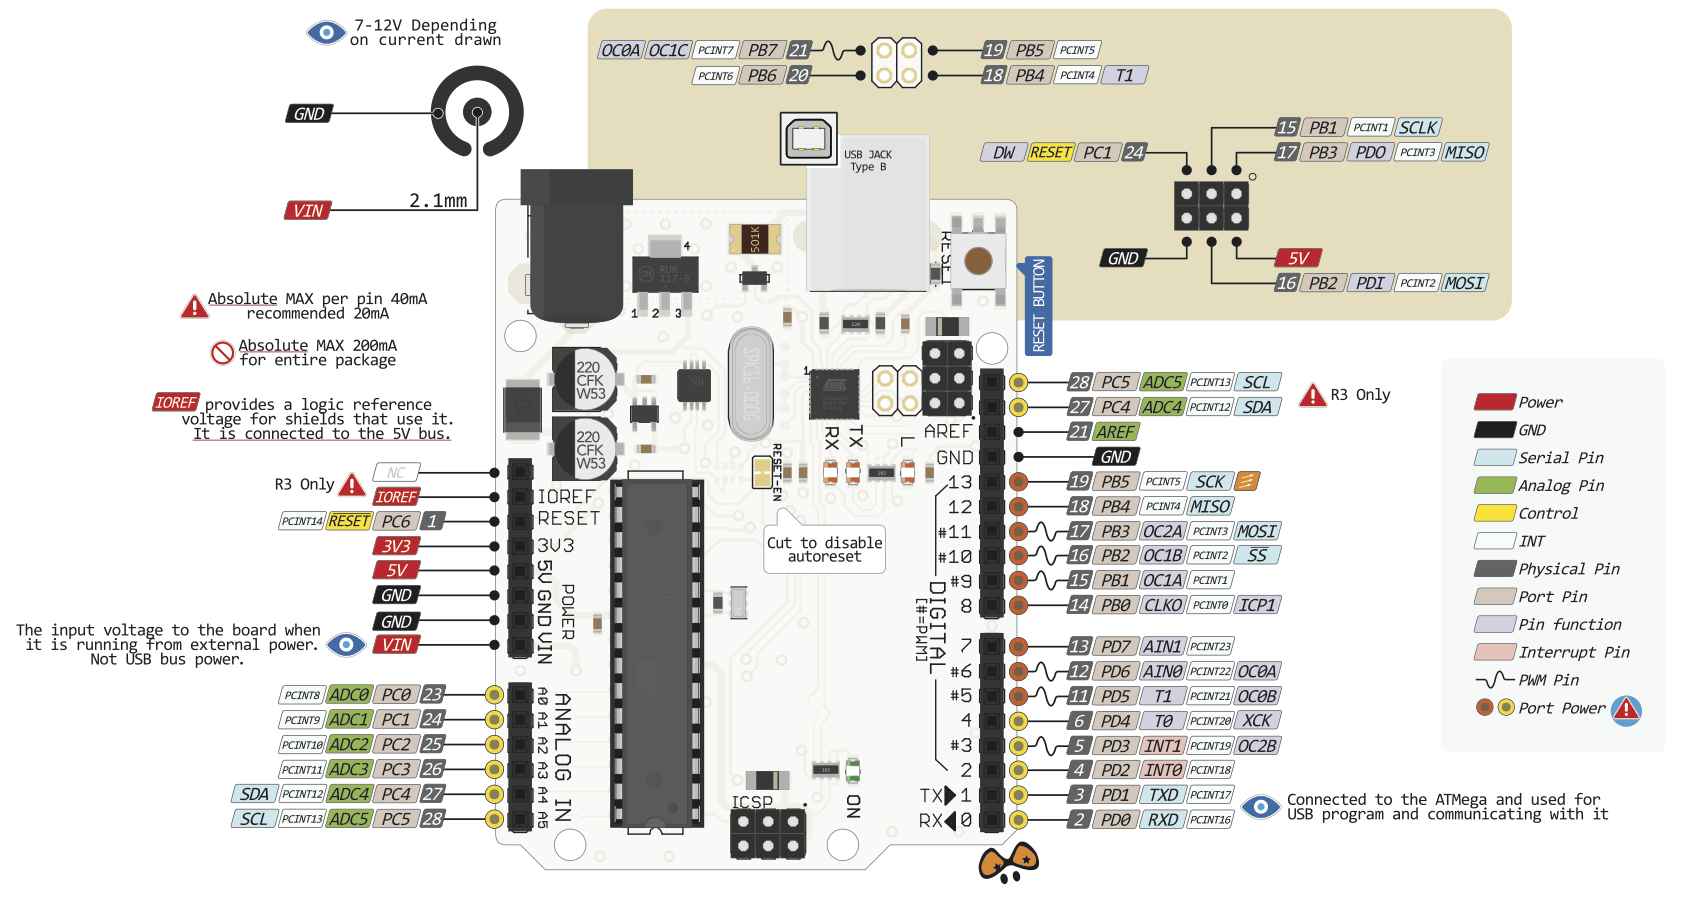
\includegraphics[width=\textwidth]{figures/arduino/portmani.PNG}
	\caption{Arduino uno med ATmega328}
	\label{fig:portmani}
	Her kan man se hvilke ben der er på Arduinoen, og hvilke porte de fordelt på ( PORTB, PORTC og PORTD). Hvis man ser på "Port pin", står der P for port, efterfulgt af bogstavet for hvilken port den er tildelt, efterfulgt af dens bit position i den port.\\
	Vi har også opgivet den påkrævede spænding for at køre Arduinoen. Vi kan også se Analog input ben (A0-A5) og de digital input og output ben (0-13). Vi kan se ud fra analog ben A4 og A5 at de er SDA og SCL, som er relevant når vi skal benytte I2C kredsen.
	\\Kilde: \url{http://pighixxx.com/unov3pdf.pdf}
\end{figure}
\subsubsection{Analog inputs og outputs (PWM)}\label{sec:ard:analog}
Analog input i Arduinoen er et input som beskriver spændingsfaldet over inputtet og jord med et 10 bit tal.\cite{arduinoAnalog} Dette betyder at den laveste værdi og højeste værdi af et analog input er
\begin{align}
\SI{}{U_{MIN}}&=b00\,0000\,0000\rightarrow 0\rightarrow \SI{0}{V}\\
\SI{}{U_{MAX}}&=b11\,1111\,1111\rightarrow 1023\rightarrow \SI{5}{V}\\
\end{align}
Med Arduinoen kan man få et analog input igennem en analog ben (se \ref{fig:portmani}), og kalde metoden \emph{analogRead()} til benets nummer, eksempelvis A0. Da vores precision er på 10 bit, til at beskrive et maks spændingsfald på $\SI{5}{V}$, må det gælde at den laveste ændring i spændingsfaldet vi kan måle er
\begin{align}
U_{prec}&=\frac{\SI{5}{V}}{1023}\approx \SI{5d-3}{V}
\end{align}
\subsubsection{Digital inputs og outputs}
Digital input på Arduinoen er en boolean værdi, som enden kan være sand eller falsk (også kendt som TRUE/FALSE eller HIGH/LOW). Disse værdier reflektere den digitale logik på det digitale ben, som fungere således: når spændingsfaldet mellem bennet og jord er $\SI{5}{V}$ er værdien sand og når spændingsfaldet er $\SI{0}{V}$ er den falsk. Mere præcist skifter værdien mellem at være sand og falsk ved omkring $\SI{3}{V}$, på $\SI{5}{V}$ logik Arduinoer. \cite{arduino:dig}\\
\\
Et digital output følger samme logik, her der sætter man dog udgangsspændingen på bennet. Det betyder altså at hvis man sætter et digital ben til sandt, vil udgangsspændingen på bennet være $\SI{5}{V}$ og hvis man sætter det til falsk vil det være $\SI{0}{V}$. \cite{arduino:dig}\\
\\


\subsubsection{I2C - Synkroniseret kommunikation}


%-------------------------------------------------------------------------------------------------------------------------------------------
%--------------------------------------- PROGRAMMING PART ----------------------------------------------------------------------------------
%-------------------------------------------------------------------------------------------------------------------------------------------
\subsection{Kort beskrivelse af programmets formål}
\subsubsection{Master Arduino}
Vores Master Arduino står for styring af motorerne, ladningssensor og hastighedssensor. Programmet til Master Arduinoen skal kunne kommunikere med Controlleren, så den kan se om der skal rygges op eller ned på kanonen eller om der skal affyres. Den skal også kunne bestemme farven af bolden i røret og om der faktisk er en bold i røret. Når bolden bliver affyret skal hastigheden af bolden også kunne bestemmes. Til sidst skal den kunne sende information som farven af bolden, hældningen af kanonen og hastigheden af bolden til Controlleren, så det kan skrives på displayet.
\subsubsection{Controller Arduino}
Controller Arduinoen skal kunne sende data om knappernes tilstand og kunne modtage data om hvad der skal stå på displayet. Da vores bruger benytter Controlleren til at styre kanonen, skal forsinkelsen imellem at man trykker på en knap, til at kanonen ryger sig være relativ lille.\\
\\
\\
\\
Programmet til master Arduinoen kan fines i bilag \ref{bilag:programMaster} og Controller Arduinoen i bilag \ref{bilag:programController}, som er kommenteret. De mest komplekse og primære funktioner vi har programmeret, er beskrevet i sektion \ref{sec:primaerefunc}.
\subsection{Oversigt over inputs og outputs og lokation}
\begin{table}[H]
	\caption{Inputs og outputs for Master Arduinoen} % title
	\label{tab:IOMaster}
	\centering
		\begin{tabular}{c|c c} 
		Ben & I/O & Forbundet komponent\\ [0.5ex] 
		\hline 
			2 & Output & Stepper motor\\
			3 & Output & Stepper motor\\
			4 & Output & Stepper motor\\
			5 & Output & Stepper motor\\
			6 & Output & Trækmotor\\
			9 & Output & Gearmotor (fri)\\
			10 & Output & Gearmotor (lås)\\
			11 & Output & Ladningssensor LED (grøn)\\
			12 & Output & Ladningssensor LED (rød)\\
			13 & Output & Ladningssensor LED (blå)\\
			A0 & Input & Ladningssensor Fotodiode\\
			A1 & Input & Hastighedssensor 1\\			
			A2 & Input & Hastighedssensor 2\\
			A4 (SDA) & I/O & I2C kommunikation (data)\\
			A5 (SCL) & I/O & I2C kommunikation (clock)\\[1ex]
		\hline %inserts single line
	\end{tabular}
\end{table}

\begin{table}[H]
	\caption{Inputs og outputs for Controller Arduinoen} % title
	\label{tab:IOController}
	\centering
		\begin{tabular}{c|c c} 
		Ben & I/O & Forbundet komponent\\ [0.5ex] 
		\hline 
			2 & I/O & LCD (DB7)\\
			3 & I/O & LCD (DB6)\\
			4 &I/O & LCD (DB5)\\
			5 &I/O & LCD (DB4)\\
			11 & Output & LCD (E)\\
			12 &Output & LCD (RS)\\
			A0 & Input & Knap (ryg kanon op)\\
			A1 & Input & Knap (ryg kanon ned)\\			
			A2 & Input & Knap (affyre bold)\\
			A4 (SDA) & I/O & I2C kommunikation (data)\\
			A5 (SCL) & I/O & I2C kommunikation (clock)\\[1ex]
		\hline %inserts single line
	\end{tabular}
\end{table}
\todo{ret det med I2C ben}
\subsection{Primære funktioner}\label{sec:primaerefunc}
\subsubsection{1}
\subsubsection{2}
\subsubsection{3} 
\input{files/chapters/2_4Test}

%%%%%%% Forbedring af produktet %%%%%%%%
\section{Fremstilling}

\subsection{Fumlebræt-modeller}
	\begin{figure}[H]
		\centering
	    
\includegraphics[width=13cm]{figures/stock.jpg}
		\caption{}
		\label{fig:}
	\end{figure}
\subsection{PCB - fremstilling}\label{subs:pcbfremstilling}
	\begin{figure}[H]
		\centering
	    
\includegraphics[width=13cm]{figures/stock.jpg}
		\caption{Et billede af et PCB vi designede i Livewire}
		\label{fig:PCBPrint}
	\end{figure}
	\begin{figure}[H]
		\centering
	    
\includegraphics[width=13cm]{figures/stock.jpg}
		\caption{Et billede af et PCB fremstillet fysisk}
		\label{fig:PCBfysisk}
	\end{figure}
\subsection{Endelige prototype}\label{subs:endeligProto}
\begin{figure}[H]
	\centering
    
\includegraphics[width=13cm]{figures/stock.jpg}
	\caption{Billede af endelig produkt}
	\label{fig:endeligPrototype}
\end{figure}
\todo{Beskriv hvordan PCB-baseret produkt ikke fungrede, har vi nogen mulige forklaringer?}

\section{Slut afprøvning} \label{sluttest}
\todo{Få skrevet om hvorfor bolden ikke passede}
\section{Videreudvikling}
Der er to typer af forbedringer der som skal til før man har et endeligt produkt. Først skal alle de dele som voros prototype burde kunne klare laves. Bagefter kan man begynde at lave produktet mere brugervendeligt.\\

For at få prototypen til at virke skal selve kanon designet laves om. Dette kan gøres ved at tage den mekanisme der skal hive i elastikkerne og placere dem mere direkte bag ved kanonrøret for at undgå for mange unødige kræftpåvirkninger på resten af kanonen.\\
Udover dette er det nødtvendigt at bruge et mindre rør der har en størrelse der svarer til størelsen på bolden således at farvesensoren ikke opfanger farver fra selve røret og omgivelserne. Hertil ville det også være smart at male indersiden af røret sort.\\
Det ville sandsynligvis være en god ide at lave produktet af metal og 3D printet plastik ved et fremtidigt produkt da det giver mulighed for at producere lagt mere specialiserede dele. \\
For sikkerhed er det en god ide at finde en løsning til at produktet har mulighed for at gå i stykker hvis man vinkler kanonen for kraftigt. Dette kunne blive gjort ved at bruge gear som har en maksimum drejningsmoment som de kan klare før de begynger at skippe nogle tænder. Eller man kunne have nogle flere knapper for at se om kanonen har flyttet sig helt til en side.\\
Udover dette kunne man lave controlleren både mere stabil ved at lave et PCB og lave en ramme til den så man holde den behageligt i hånden.

\section{Prisliste}
\subsection{Produktionsomkostninger}
% KONDENSATORER
% 10
% 10
% 100
% 1000
% NANOFARAD
% 0.18$ * 4
% http://uk.rs-online.com/web/p/polyester-film-capacitors/6224634/?searchTerm=622-4634&relevancy-data=636F3D3126696E3D4931384E525353746F636B4E756D6265724D504E266C753D656E266D6D3D6D61746368616C6C26706D3D5E283F69292852537C5253207C52532D293F5C647B337D285C73293F5B5C732D2F255C2E2C5D285C73293F5C647B332C347D2426706F3D313426736E3D592673743D52535F53544F434B5F4E554D4245522677633D4E4F4E45267573743D3632322D34363334267374613D3632323436333426

% RESISTORER
% De koster omtrent det samme 
% 20 i alt


% MIKROCHIPS
% HEF4001 0.1812$ https://www.arrow.com/en/products/hef4001bt652/nexperia
% MCP 601 TIMES 5 microchip 0.36$
% Fototransistor BPW21 $6.2599 https://www.verical.com/pd/vishay-photodiode-BPW21R-234268?utm_source=FindChips&utm_medium=invListing&utm_campaign=FC2015
% SWITCHES 3, 2.00$ https://www.adafruit.com/product/367
% 


% arduino 21.91 $ Dollars
% http://uk.rs-online.com/web/p/processor-microcontroller-development-kits/1240656/
% Lego motor https://shop.lego.com/en-DK/LEGO-Power-Functions-XL-Motor-8882 
% 14$

% Steppermotor
% http://uk.rs-online.com/web/p/stepper-motors/1918328/
% 30.70 US Dollar



For at estimerer omkostninger antages det at der skal produceres 100 stykker legetøj. Ydermere antages det at de forskellige modstande der benyttes koster omtrent det samme og at kondensatorerne koster omtrent det samme 


%-------------------- Begin Table ------------------------------
\begin{table}[H] 
	\caption{Omkostningspris for prototype} % title
	\label{tab:omkostning}
	\centering
		\begin{tabular}{c|c c c c} 
		
		Komponent & Stk. pr. produkt & Pris stk. [USD] & Kilde & Samlet pris [USD]\\ [0.5ex] 
		\hline 
			PCB & - & 5.81 & \cite{price:PCB} & 5.81\\ 
			Resistorer & 20 & 0.01& \cite{price:resistor} & 0.2\\
			Kondensatorer & 5 &  0.18 & \cite{price:capacitor} & 0.9\\
			MCP601 & 5 & 0.36& \cite{price:MCP601} & 1.8\\
			HEF4001 & 1 &0.18& \cite{price:HEF4001} & 0.18\\
			BPW21 & 1 &6.26& \cite{price:BPW21} & 6.26 \\
			Steppermotor &1 & 31 & \cite{price:stepper}&31 \\
			DC motor & 2 & 14 & \cite{price:dcmotor} &28 \\ 
			Arduino & 2 & 30 &\cite{price:arduino} & 60 \\
			Kanon-konstruktion & 1 & 8.81 & Estimat & 8.81 \\
			Total pris & - &- & - & 142.95\\[1ex]
		\hline %inserts single line
	\end{tabular}
\end{table}
%-------------------- End table ------------------------------
Den totale pris angivet på Tabel \ref{tab:omkostning} svarer til omtrent $\SI{970}{DKK}$, hvilket er rigtig meget for et legetøj. Men der er væsentlige måder at sænke denne pris på. F.eks. i stedet for at benytte hele Arduino UNO benytter dens microcontroller ATmega328P. Disse kan fås til en ret lav prisleje på under 2 dollars (Se kilde: \cite{price:atmega}). Hvilket sænker prisen med omtrent \SI{58}{USD}. Dette gør at et bedre estimat svarer til \SI{84.95}{USD} som er på nuværende tidspunkt ækvivalent med \SI{578.23}{DKK}. Hvilket er en mere rimelig pris.


% ATMEGA328

\subsection{Estimering af udsalgspris}
En rimelig avance vurderer vi til at være på 30\%, heraf bliver den samlede salgspris:
%-------------------- Begin Table ------------------------------
\begin{table}[H] 
	\caption{Salgspris} % title
	\label{tab:salg}
	\centering
		\begin{tabular}{c c} 
		\hline\hline
			Omkostningspris & \SI{578.23}{DKK}\\ 
			Avance & \SI{173.469}{DKK}\\
			\hline \\
			Pris uden moms & \SI{751.70}{DKK} \\
			Pris med moms & \SI{939.625}{DKK} \\[1ex] % [1ex] adds vertical space
		\hline %inserts single line
	\end{tabular}
\end{table}
%-------------------- End table ------------------------------
\subsection{Konkurrencedygtighed}
Vores produkt minder ikke meget om nuværende alternativer til Angry Birds spillet, men det tætteste er nok modeller udviklet af LEGO.
LEGO har lavet et Angry Birds spil som legetøj koncept, dog uden nogen avanceret affyringsmekanisme eller andet elektronik, hvor man kan affyrer fugle mod legoborge. Disse legomodeller kan koste hele vejen op til \SI{700}{DKK} (kilde: \cite{price:legoBird}), men vi vurderer at vores produkt er i forhold til de dyre LEGOmodeller. Dog er det meget muligt at vores produkt bliver væsentligt dyre end \SI{939.625} hvis man også skal gøre det ligeså æstetisk som LEGO's Angry birds.


%%%%%% Opsummering og evaluering %%%%%%%
\section{Konklusion}
\section{Evaluering}



%---------- BIBLIOGRAFI ----------
\addcontentsline{toc}{section}{Referencer}
% \section{Litteraturliste}
\nocite{*}
% \printbibliography[title={Bibliografi - Bøger},type=book]
% \printbibliography[title={Bibliografi - Websider},type=online]
% \printbibliography[title={Bibliografi - Artikler},type=article]
\printbibliography

% BILAG PÅ BEGYNDER
\newpage
\appendix



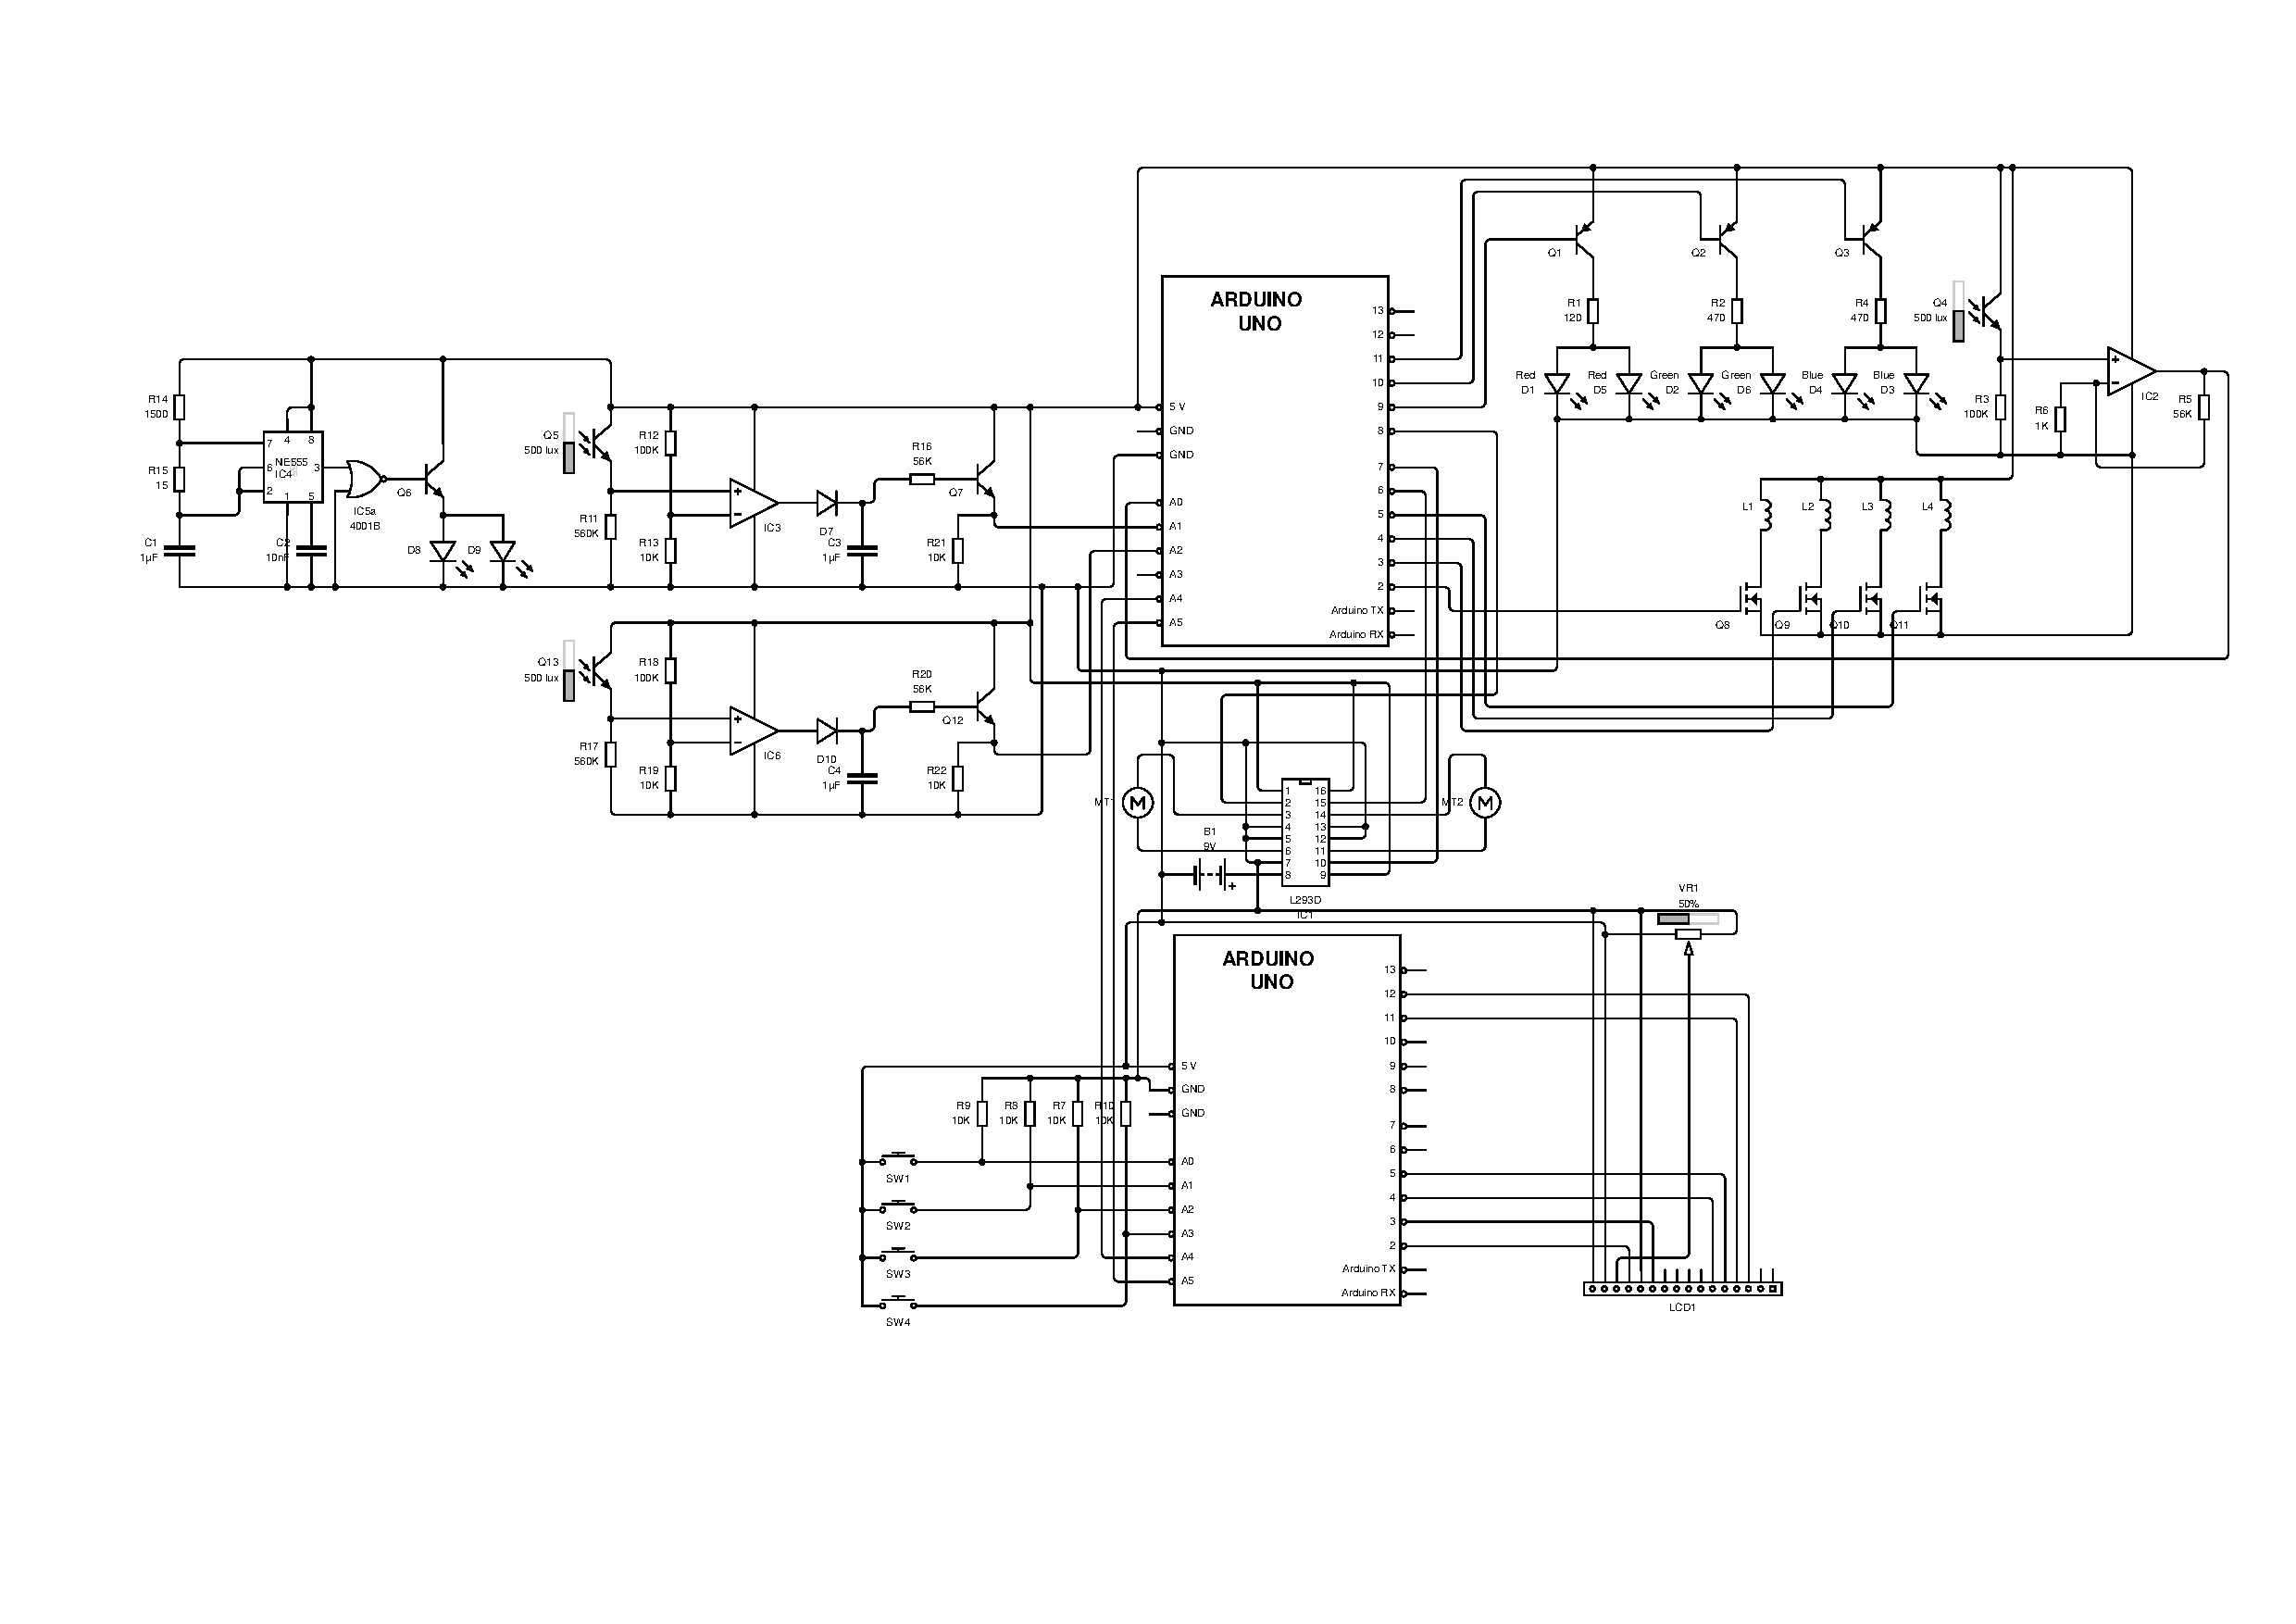
\includepdf[pages=1,fitpaper,pagecommand={\section{Samlet kredsløb} \label{bilag:samletkreds}}]{figures/CIRCUITS/samletFINAL}

% pagecommand={\section{Samlet kredsløb} \label{bilag:samletkreds}}


\section{Endelig prototype - kredsløb} \label{bilag:endeligprotokreds}
\begin{center}
	\includegraphics[width=15cm]{figures/2_5fremstilling/prototyper/Endeligproto.png}
\end{center}

\section{Endelig prototype - kanonkonstruktion} \label{bilag:endeligprotokanon}
\begin{center}
	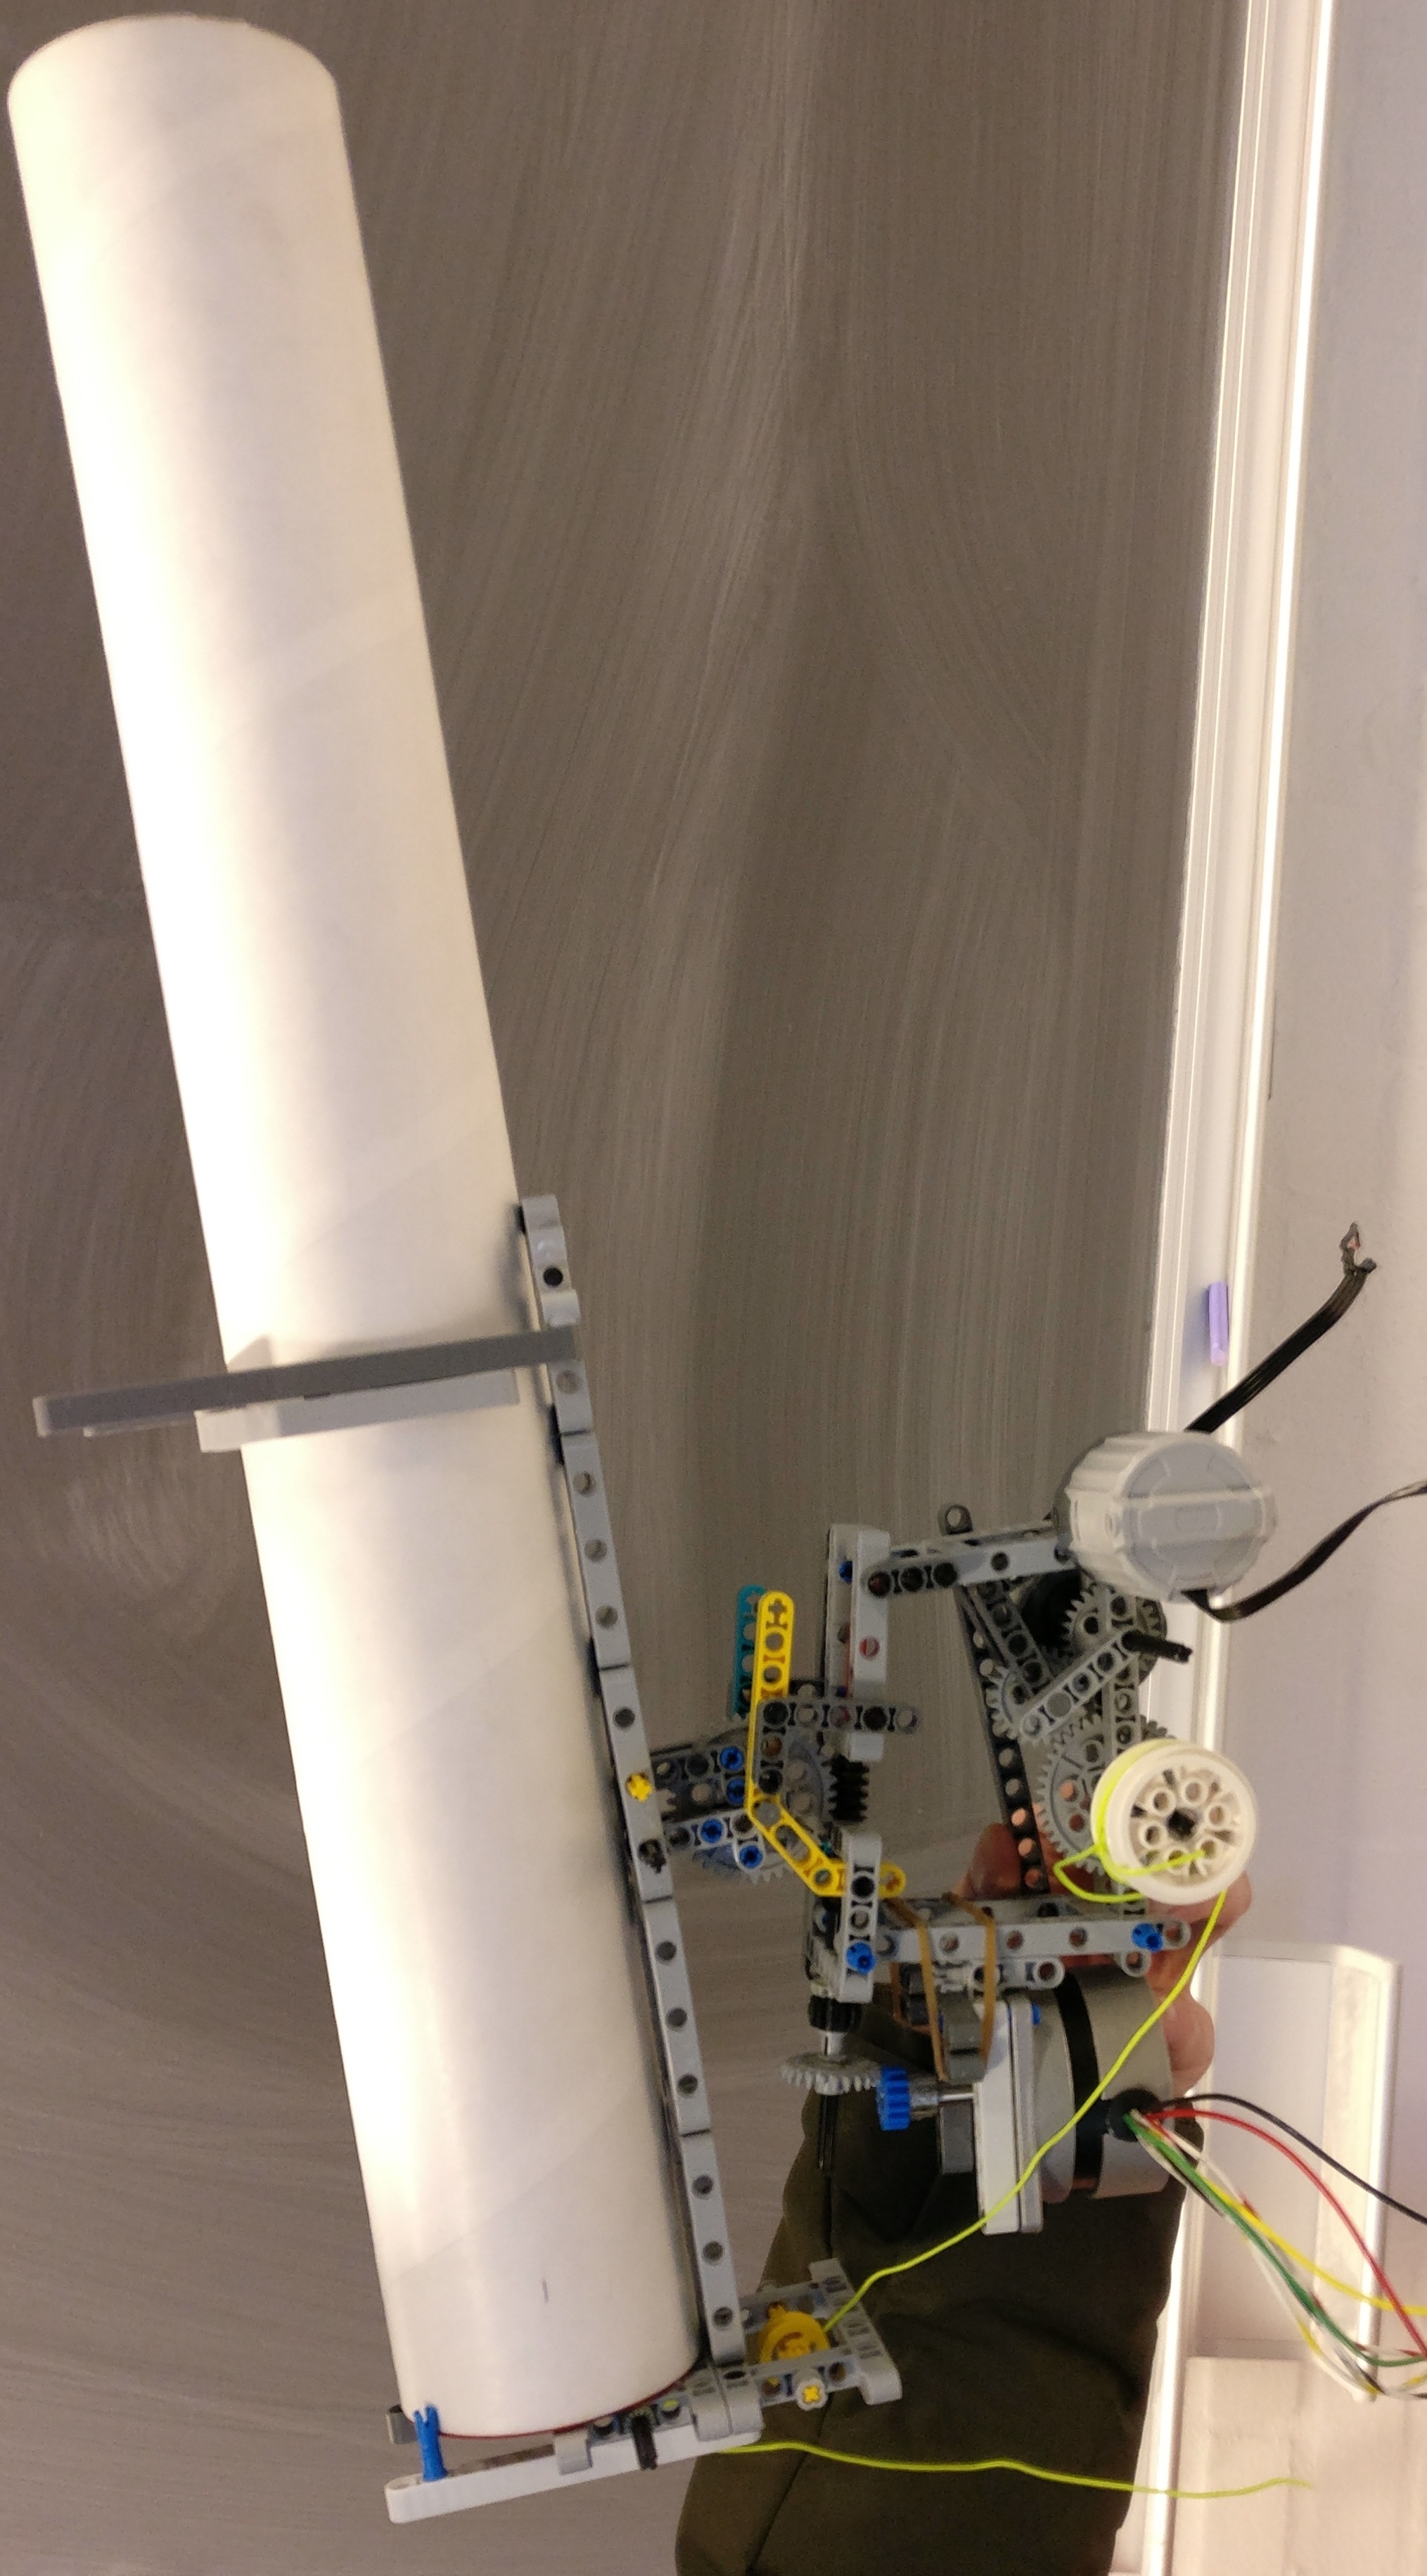
\includegraphics[height=20cm]{figures/2_5fremstilling/prototyper/paenkanon.jpg}
\end{center}
\section{PCB artwork til hastighedssensor}\label{bilag:afsenderModtagerArtwork}
\begin{figure}[H]
	\centering
    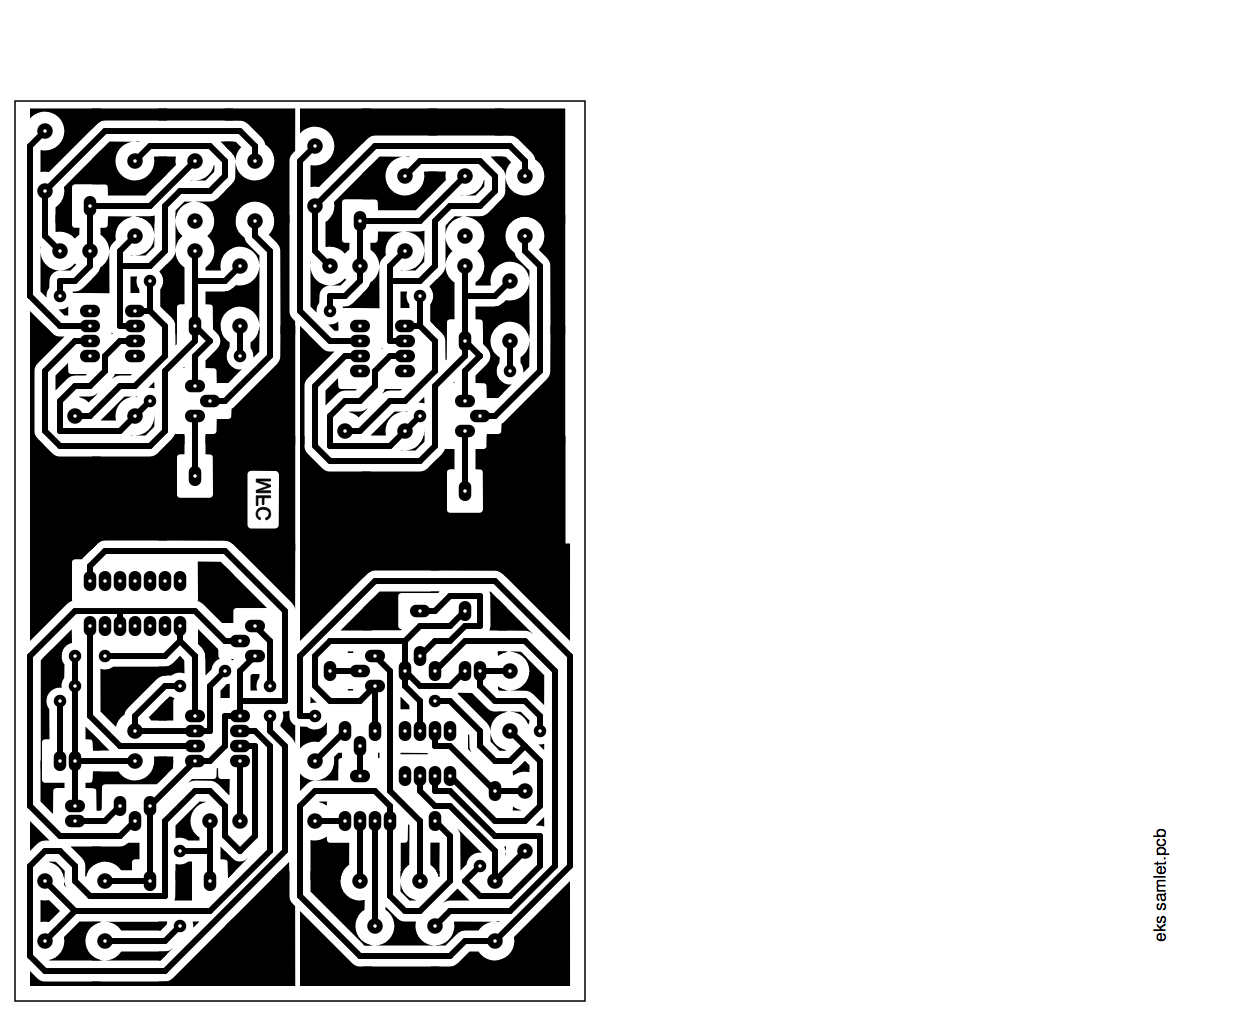
\includegraphics[width=210mm]{figures/2_5fremstilling/afsenderModtagerArtwork.png}
\end{figure}


\section{PCB artwork til arduino shield} \label{bilag:shieldArtwork}
\begin{figure}[H]
	\centering
    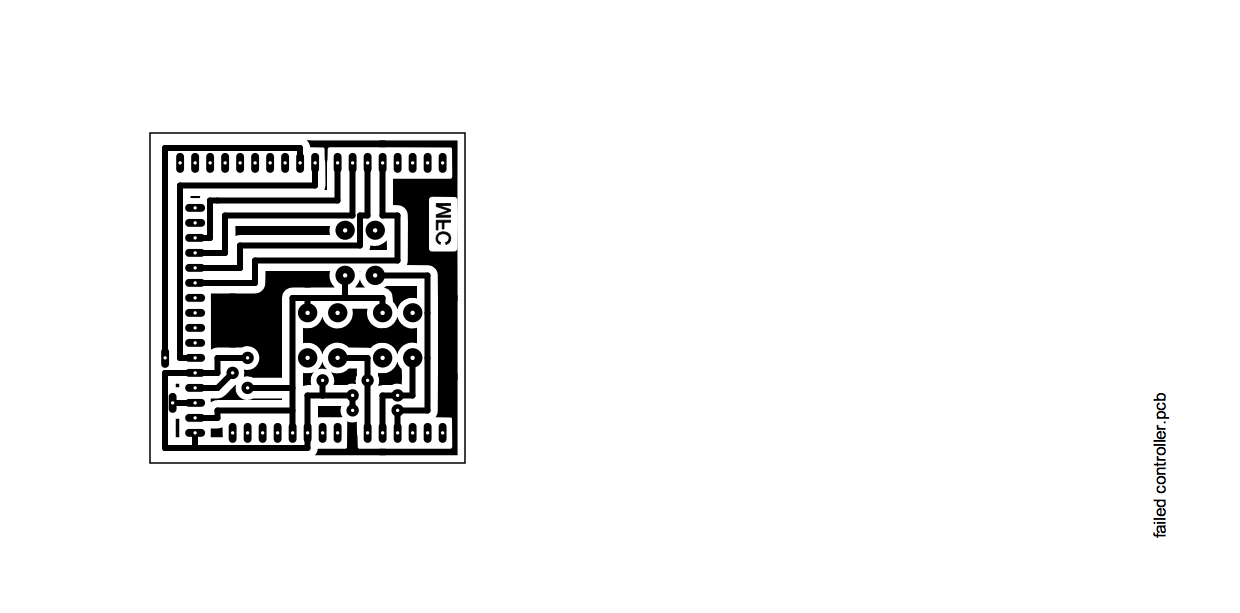
\includegraphics[width=210mm]{figures/2_5fremstilling/shieldArtwork.png}
\end{figure}

\todo{Måske skulle vi overveje at lave et nyt billede med samlede kabler}
\begin{figure}[H]
\section{Fumlebrætmodel anden del}
	\centering
    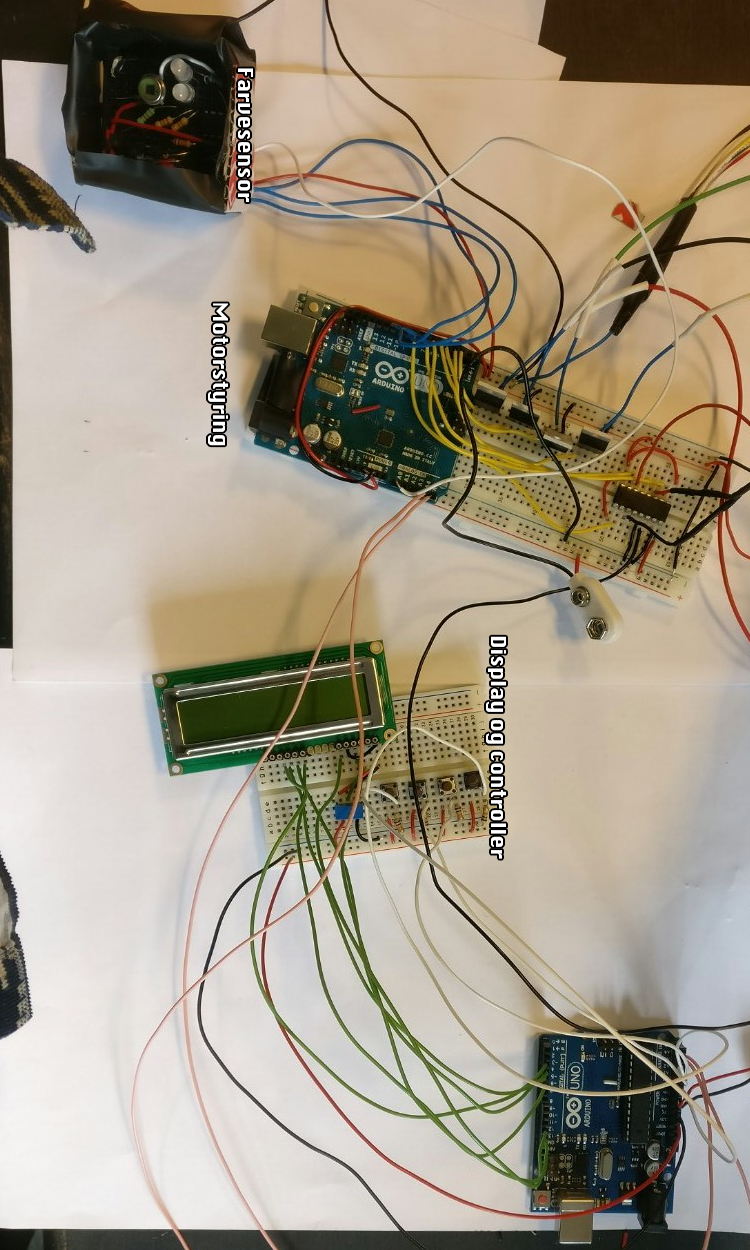
\includegraphics[width=13cm]{figures/2_5fremstilling/prototyper/rumleKreds.png}
\end{figure}


% Must be second last (the longer the later)
\section{Program til Arduino}
\label{bilag:program}
\begin{lstlisting}

\end{lstlisting}


% MUST BE LAST
\section{Logbog} 
\end{document}



